%% Преамбула TeX-файла

% 1. Стиль и язык
\documentclass{G7-32} % Стиль (по умолчанию будет 14pt)

% Остальные стандартные настройки убраны в preamble.inc.tex.
\sloppy

% Настройки стиля ГОСТ 7-32
% Для начала определяем, хотим мы или нет, чтобы рисунки и таблицы нумеровались в пределах раздела, или нам нужна сквозная нумерация.
\EqInChapter % формулы будут нумероваться в пределах раздела
\TableInChapter % таблицы будут нумероваться в пределах раздела
\PicInChapter % рисунки будут нумероваться в пределах раздела

% Добавляем гипертекстовое оглавление в PDF
\usepackage[
bookmarks=true, colorlinks=true, unicode=true,
urlcolor=black,linkcolor=black, anchorcolor=black,
citecolor=black, menucolor=black, filecolor=black,
]{hyperref}

\AfterHyperrefFix

\usepackage{microtype}% полезный пакет для микротипографии, увы под xelatex мало чего умеет, но под pdflatex хорошо улучшает читаемость

% Тире могут быть невидимы в Adobe Reader
\ifInvisibleDashes
\MakeDashesBold
\fi

\usepackage{graphicx}   % Пакет для включения рисунков

% С такими оно полями оно работает по-умолчанию:
% \RequirePackage[left=20mm,right=10mm,top=20mm,bottom=20mm,headsep=0pt,includefoot]{geometry}
% Если вас тошнит от поля в 10мм --- увеличивайте до 20-ти, ну и про переплёт не забывайте:
\geometry{right=20mm}
\geometry{left=30mm}
\geometry{bottom=20mm}
\geometry{ignorefoot}% считать от нижней границы текста


% Пакет Tikz
\usepackage{tikz}
\usetikzlibrary{arrows,positioning,shadows}

% Произвольная нумерация списков.
\usepackage{enumerate}

% ячейки в несколько строчек
\usepackage{multirow}

% itemize внутри tabular
\usepackage{paralist,array}

%\setlength{\parskip}{1ex plus0.5ex minus0.5ex} % разрыв между абзацами
\setlength{\parskip}{1ex} % разрыв между абзацами
\usepackage{blindtext}

% Центрирование подписей к плавающим окружениям
%\usepackage[justification=centering]{caption}

\usepackage{newfloat}
\DeclareFloatingEnvironment[
placement={!ht},
name=Equation
]{eqndescNoIndent}
\edef\fixEqndesc{\noexpand\setlength{\noexpand\parindent}{\the\parindent}\noexpand\setlength{\noexpand\parskip}{\the\parskip}}
\newenvironment{eqndesc}[1][!ht]{%
    \begin{eqndescNoIndent}[#1]%
\fixEqndesc%
}
{\end{eqndescNoIndent}}




% Настройки листингов.
\ifPDFTeX
% 8 Листинги

\usepackage{listings}

% Значения по умолчанию
\lstset{
  basicstyle= \footnotesize,
  breakatwhitespace=true,% разрыв строк только на whitespacce
  breaklines=true,       % переносить длинные строки
%   captionpos=b,          % подписи снизу -- вроде не надо
  inputencoding=koi8-r,
  numbers=left,          % нумерация слева
  numberstyle=\footnotesize,
  showspaces=false,      % показывать пробелы подчеркиваниями -- идиотизм 70-х годов
  showstringspaces=false,
  showtabs=false,        % и табы тоже
  stepnumber=1,
  tabsize=4,              % кому нужны табы по 8 символов?
  frame=single
}

% Стиль для псевдокода: строчки обычно короткие, поэтому размер шрифта побольше
\lstdefinestyle{pseudocode}{
  basicstyle=\small,
  keywordstyle=\color{black}\bfseries\underbar,
  language=Pseudocode,
  numberstyle=\footnotesize,
  commentstyle=\footnotesize\it
}

% Стиль для обычного кода: маленький шрифт
\lstdefinestyle{realcode}{
  basicstyle=\scriptsize,
  numberstyle=\footnotesize
}

% Стиль для коротких кусков обычного кода: средний шрифт
\lstdefinestyle{simplecode}{
  basicstyle=\footnotesize,
  numberstyle=\footnotesize
}

% Стиль для BNF
\lstdefinestyle{grammar}{
  basicstyle=\footnotesize,
  numberstyle=\footnotesize,
  stringstyle=\bfseries\ttfamily,
  language=BNF
}

% Определим свой язык для написания псевдокодов на основе Python
\lstdefinelanguage[]{Pseudocode}[]{Python}{
  morekeywords={each,empty,wait,do},% ключевые слова добавлять сюда
  morecomment=[s]{\{}{\}},% комменты {а-ля Pascal} смотрятся нагляднее
  literate=% а сюда добавлять операторы, которые хотите отображать как мат. символы
    {->}{\ensuremath{$\rightarrow$}~}2%
    {<-}{\ensuremath{$\leftarrow$}~}2%
    {:=}{\ensuremath{$\leftarrow$}~}2%
    {<--}{\ensuremath{$\Longleftarrow$}~}2%
}[keywords,comments]

% Свой язык для задания грамматик в BNF
\lstdefinelanguage[]{BNF}[]{}{
  morekeywords={},
  morecomment=[s]{@}{@},
  morestring=[b]",%
  literate=%
    {->}{\ensuremath{$\rightarrow$}~}2%
    {*}{\ensuremath{$^*$}~}2%
    {+}{\ensuremath{$^+$}~}2%
    {|}{\ensuremath{$|$}~}2%
}[keywords,comments,strings]

% Подписи к листингам на русском языке.
\renewcommand\lstlistingname{Листинг}
\renewcommand\lstlistlistingname{Листинги}

\else
\usepackage{local-minted}
\fi

% Полезные макросы листингов.
% Любимые команды
\newcommand{\Code}[1]{\textbf{#1}}



\begin{document}

\frontmatter % выключает нумерацию ВСЕГО; здесь начинаются ненумерованные главы: реферат, введение, глоссарий, сокращения и прочее.

\thispagestyle{empty}

\centerline{Министерство образования и науки РФ}
\begin{center}
САНКТ-ПЕТЕРБУРГСКИЙ НАЦИОНАЛЬНЫЙ  ИССЛЕДОВАТЕЛЬСКИЙ УНИВЕРСИТЕТ ИТМО
\end{center}


\vfill

\centerline{\LARGE{ОТЧЁТ}}
\centerline{\large{по проектно-конструкторской практике}}

\vfill

Студент Сухих Даниил  группы R34403 \hfill

Научный руководитель Власов С. М.\hfill

\vfill

\centerline{Санкт-Петербург, 2024}
\clearpage



%\listoffigures                         % Список рисунков

%\listoftables                          % Список таблиц

%\NormRefs % Нормативные ссылки 
% Команды \breakingbeforechapters и \nonbreakingbeforechapters
% управляют разрывом страницы перед главами.
% По-умолчанию страница разрывается.

% \nobreakingbeforechapters
% \breakingbeforechapters
%\TechTask
\thispagestyle{empty}
Объектом исследования является бесколлекторный двигатель постоянного тока без установленных датчиков Холла, имеющий трапезоидальный характер противо-ЭДС.

Основной целью работы является разработка алгоритма для управления такого рода двигателями.

Для достижение цели поставлены следующие задачи: 
 1. Исследование существующих подходов к управлению и обзор существующих технических решений
 2. Синтез алгоритма и создание модели его реализации в программном комплексе Matlab/Simulink. Требования, предъявялемые к алгоритму: перерегулирование - 30 \%; время переходного процесса - 0,4 с; максимальная установившаяся ошибка - 1 \%
 3. Разработка печатной платы для реализации готового алгоритма в приложении Altium Designer, подготовка файлов к её изготовлению и изготовление. Требование, предъявляемые к разрабатваемой схеме: напряжение питания - 12 В; максимальный ток силовой части - 5 А; максимальная частота ШИМ - 20 кГц; наличие на плате контактов для подключения выходов микроконтроллера, на котором будет реализован алгоритм
 4. Экспериментальная 

Основными задачами работы являются синтез алгоритма управления такими двигателями, его проверка в ходе моделирования и реализация готового устройства, реализуещего полученный алгоритм.

Решение первых двух задач (синтез алгоритма, моделирование) будет проводиться с использованием программного комплекса Matlab/Simulink.

Требования к разрабатываемому алгоритму:
\begin{enumerate}
	\item Перерегулирование - $30$ \%
	\item Время переходного процесса - $0,4$ c
	\item Максимальная установившаяся ошибка - $1$ \% 
\end{enumerate}

Для решения последней задачи будет задействовано приложение Altium Designer для разработки схемы, её проверки и дальнейшей подготовки к изготовлению печатной платы.

Требования к разрабатываемой схеме:
\begin{enumerate}
	\item Напряжение питания схемы и двигателя  - $12$ В, максимальный ток силовой части - $5$ А
	\item Максимальная частота ШИМ - $20$ кГц
	\item Алгоритм управления реализуется на микроконтроллере, поэтому на плате должны быть контакты для подключения его пинов
\end{enumerate}

Также в ходе работы будут дополнительно рассмотрены следующие вопросы:
\begin{enumerate}
	\item Обзор существующих алгоритмов и аналогов разрабатываемого устройства
	\item Специфика работы бесколлекторных двигателей и принцип их управления
\end{enumerate}




\tableofcontents
\thispagestyle{empty}

\Introduction
\thispagestyle{empty}

Бесколлекторные двигатели постоянного тока – это тип двигателей постоянного тока, которые обладают большей эффективностью, надежностью и меньшими габаритами по сравнению с традиционными двигателя постоянного тока \cite{book.itmo_motors}. В связи с этим они сейчас обретают всё большую популярность, когда речь идёт о компактности, энергоэффективности и уменьшении веса и используются в большинстве современных электронных устройств, применяются во многих сферах, в том числе в робототехнике, медицинских приборах и инструментах. 

Однако стоит отметить и один недостаток: необходимость специального драйвера для обеспечения его вращения и регулирования. В связи с чем усложняются конструкция и эксплуатация (появляется больше необходимых для обслуживания узлов). Но с развитием полупроводниковых компонентов эта проблема уходит на второй план и компенсируется преимуществами таких двигателей, которые были описаны ранее.

Поэтому главной задачей и целью данной работы является разработка системы управления такого рода двигателями для обеспечения заданных показателей качества. В ходе работы будет синтезирован алгоритм коммутации обмоток двигателя и управления им в программной среде Matlab/Simulink. После чего будет разработано и изготовлено готовое устройство для проверки полученного алгоритма на практике. 

Далее будут рассмотрены существующие алгоритмы управления бесколлекторными двигателями и технические реализации алгоритмов функционирования подобных устройств с целью формирования собственного технического решения.






\mainmatter % это включает нумерацию глав и секций в документе ниже

\chapter{Управление бесколлекторным двигателем}
\label{cha:chap1}

\section{Устройство двигателя и принцип работы}
\label{sec:bldc_theory}

В основе коллекторных двигателей постоянного тока лежит механический механизм коммутации обмоток с использованием щёток, изменяющим направление тока в обмотках якоря для формирования постоянного момента. Из-за этого возникают электромагнитные и акустические шумы, появляется потребность в довольно частом обслуживание щеточно-коллекторного узла из-за износа, возникающего в следствии трения механических частей и искрения в процессе коммутации. \cite{book.kim_motors}

Чтобы преодолеть эту проблему, были разработаны бесколлекторные двигатели (БДПТ). По своей структуре они по сути являются синхронными двигателем с сосредоточенным распределением и магнитоэлектрическим возбуждением обмоток статора, но которые также питаются от постоянного тока. В данном типе двигателей коммутация обмоток происходит не механическим способом, а электрическим. Для электрической коммутации зачастую ипользуются датчики положения ротора и специлизированные управляющие схемы на основе управляемых ключей (транзисторов). \cite{book.itmo_motors,book.kim_motors}

\begin{figure}[!h]
\centering
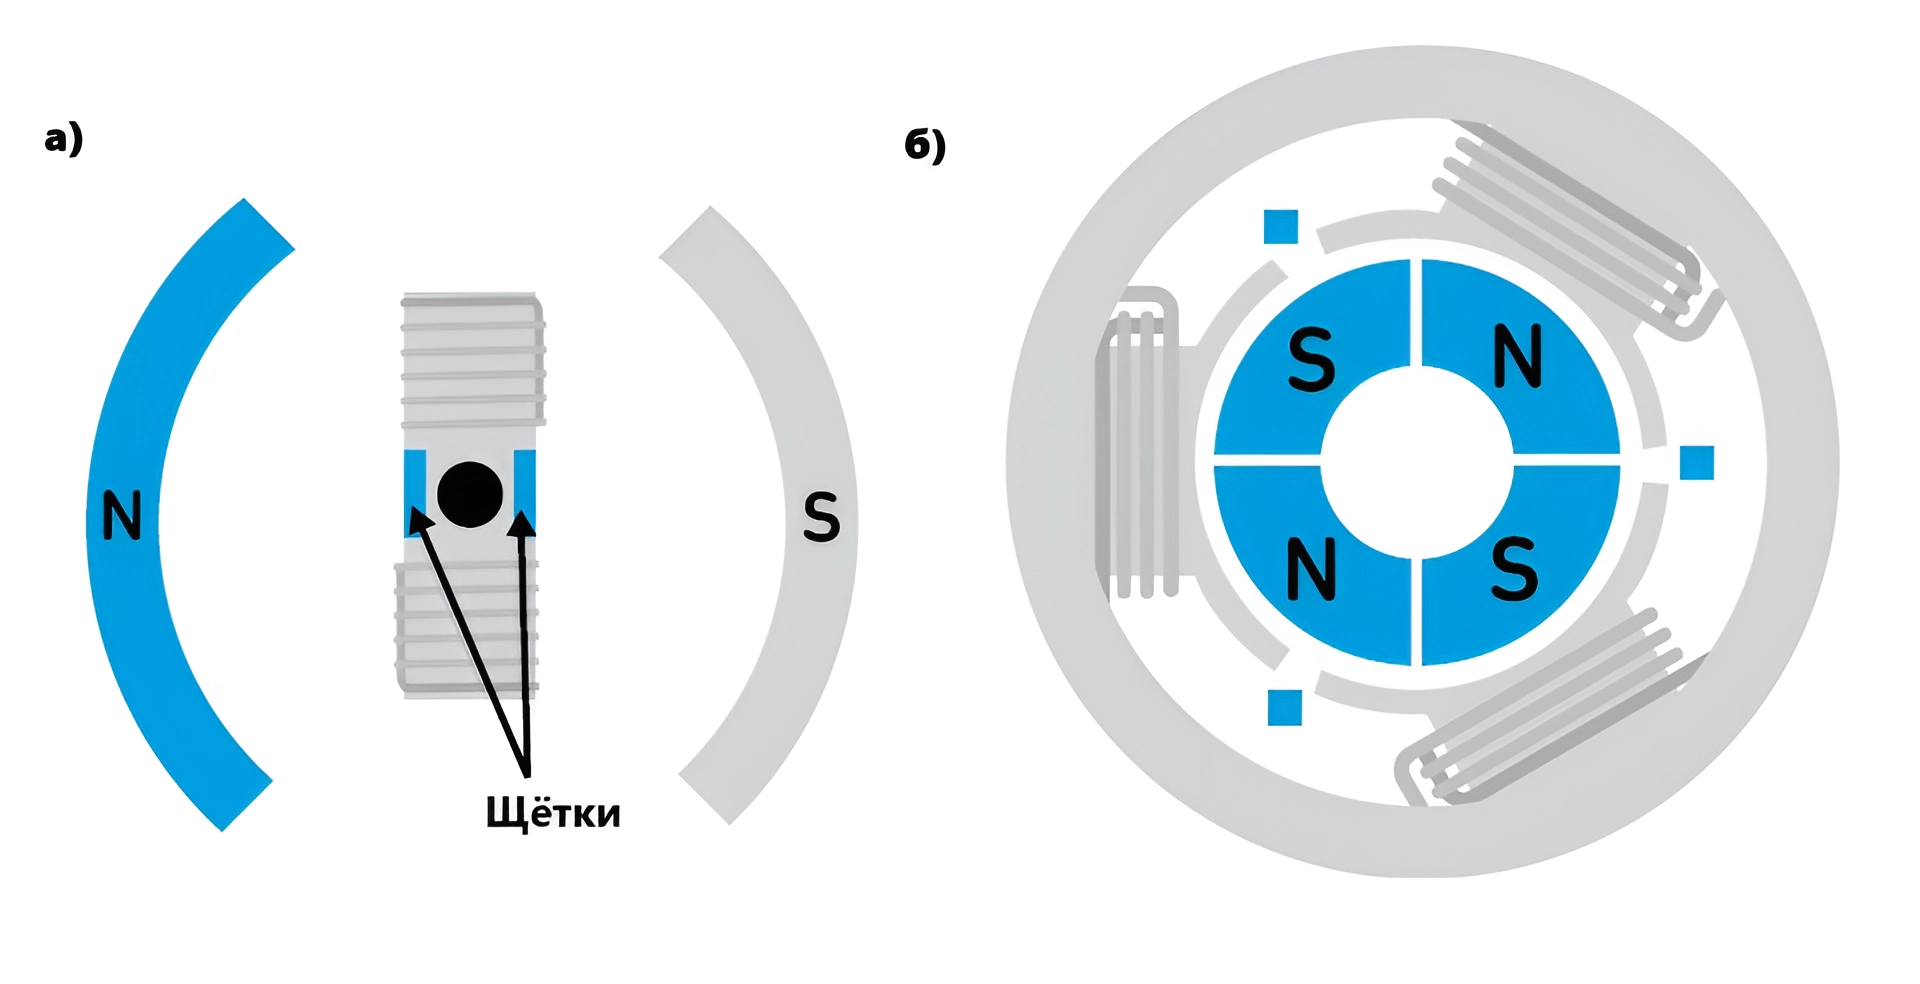
\includegraphics[width=0.7\textwidth]{inc/img/dc_and_bldc.png}
\caption{Структура двигателей постоянного тока: а - коллекторный дпт, б - бесколлекторный дпт \cite{book.bldc_dummy}}
\end{figure}

Данные двигатели часто сравнивают с синхронными машинами с постоянными магнитами (вентильные двигатели или синхронные машины с постоянными магнитами). Однако последние имеют распределённую обмотку статора и питаются от переменного тока, из-за чего имеют синусоидальный харакетри противо-ЭДС в обмотках. Тогда как в БДПТ двигателе она имеет трапецеидальный характер. Ввиду этих особенностей к этим двигателям применяются разные алгоритмы управления и разные драйверы. Для вентильных двигателей алгоритмы управления имеют более сложный характер.

\begin{figure}[!h]
\centering
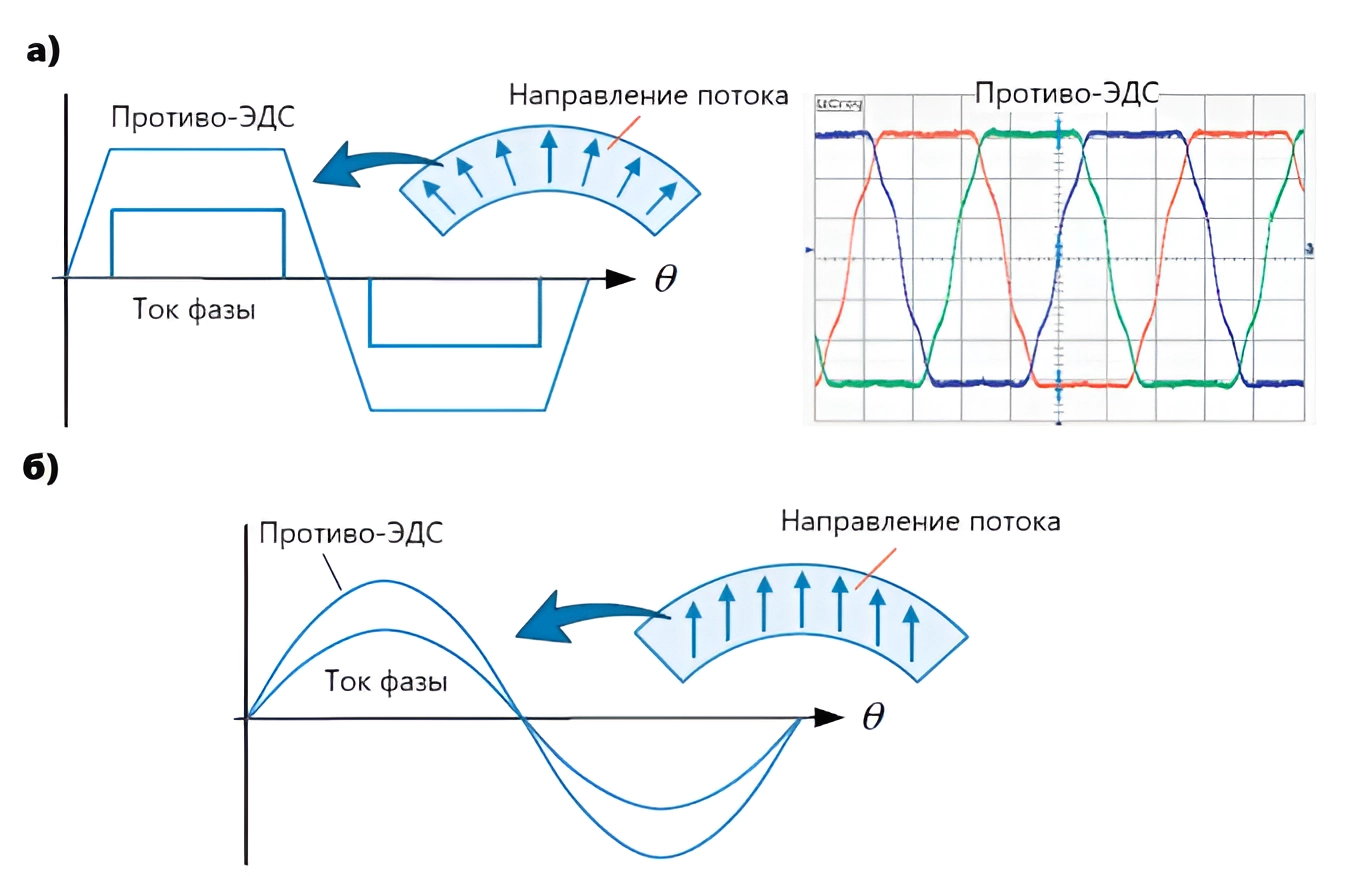
\includegraphics[width=0.7\textwidth]{inc/img/bldc_and_pmsm.png}
\caption{Вид противо-ЭДС: а - бесколлекторный дпт, б - вентильный двигатель \cite{book.kim_motors}}
\end{figure}

В итоге, бесколлекторные двигатели постоянного тока обладают большей эффективностью из-за меньших затрат на коммутацию, большей надёжностью из-за отсутствия щеточно-коллекторного узла, меньшими габаритами при сравнимой мощности (большей плотностью мощности) и меньшей стоимостью из-за более простой конструкциии в сравнении с традиционными двигателями постоянного тока.

\section{Управление на основе датчиков Холла}
\label{sec:hall}
BLDC двигатель можно представить в виде трёх соединенных между собой обмоток. Одновременно можно пропускать ток через 2 из 3 обмоток, что позволяет создать 6 направлений вектора магнитного поля статора, изображенные на Рисунке \ref{img:mag_field}.

\begin{figure}[!h]
\centering
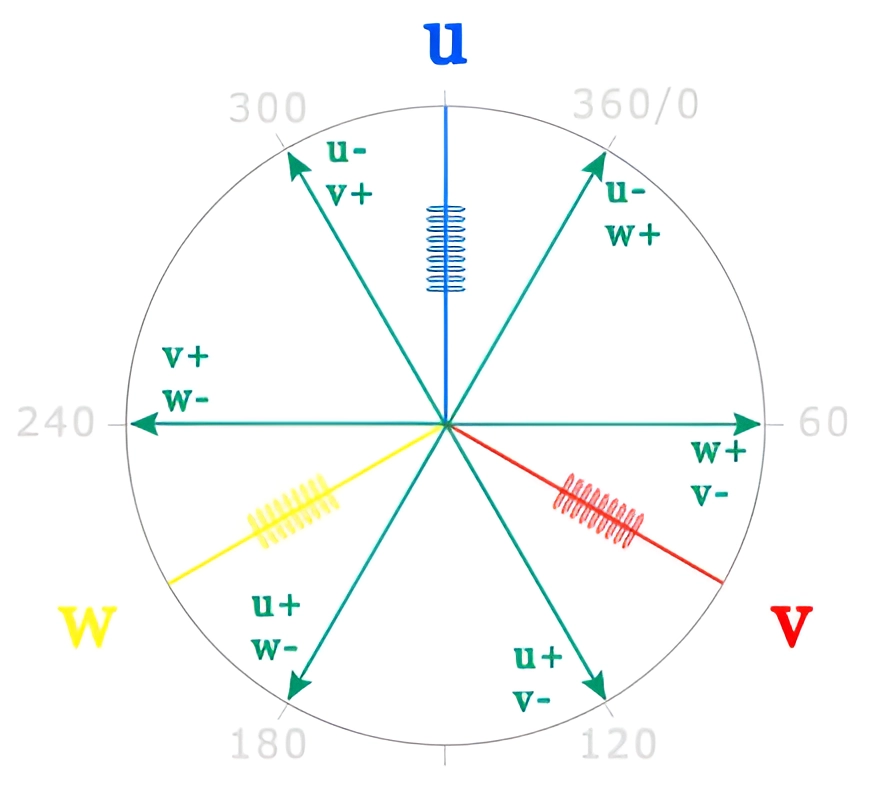
\includegraphics[width=0.7\textwidth]{inc/img/bldc_vec.png}
\caption{Возможные направления векторов магнитного поля, создаваемого статором bldc двигателя (U, W, V --- выходы обмоток двигателя) \cite{habr:bldc_control}}
\label{img:mag_field}
\end{figure}

Таким образом, для управления необходимо вовремя коммутировать фазы обмоток, создавая круговое магнитное поле. Из этого можно получить закон коммутации из 6 шагов (по количеству возможных комбинаций протекания тока через обмотки). Возможная последовательность коммутации обмоток приведена в Таблице \ref{table:commutation}.

\begin{center}
\captionof{table}{Возможная таблица коммутации обмоток (U, W, V --- выходы обмоток двигателя)\label{table:commutation}}
\begin{tabular}{|c|c|c|}
 \hline
 DC + & DC - & Не подключена \\
 \hline
 W & U & V \\ 
 \hline
 W & V & U \\
 \hline
 U & V & W \\
 \hline
 U & W & V \\
 \hline
 V & W & U \\
 \hline
 V & U & W \\
 \hline
\end{tabular}
\end{center}

Но как можно определить момент, в который необходимо изменить направление протекания тока в обмотках (перейти к следующему шагу цикла)? Самое простое в плане реализации системы управления является установка специальных датчиков, работающих на эффекте Холла. Они обычно располагаются под $120$ электрических градусов друг от друга, чтобы за один цикл коммутации получить все возможные комбинации состояний датчиков (кроме состояний, когда все сработали или ни один не сработал, что невозможно в работающием двигателе в силу их расположения). Стоит отметить, что $360$ электрических градусов соответствуют одному периоду магнитного поля.

Для определения механических градусов (то есть расположения на самом статоре) необходимо знать число пар полюсов двигателя ($N$) и воспользоваться формулой: $\dfrac{360}{3N}$. Например, в однополюсном двигателе датчики располагаются под углом в $120^{\circ}$, в двухполюсном --- $60^{\circ}$ и т. д. Таким образом, для одного механического оборота двигателя необходимо выполнить количество циклов коммутации, равное числу пар полюсов двигателя.

\begin{figure}[!h]
\centering
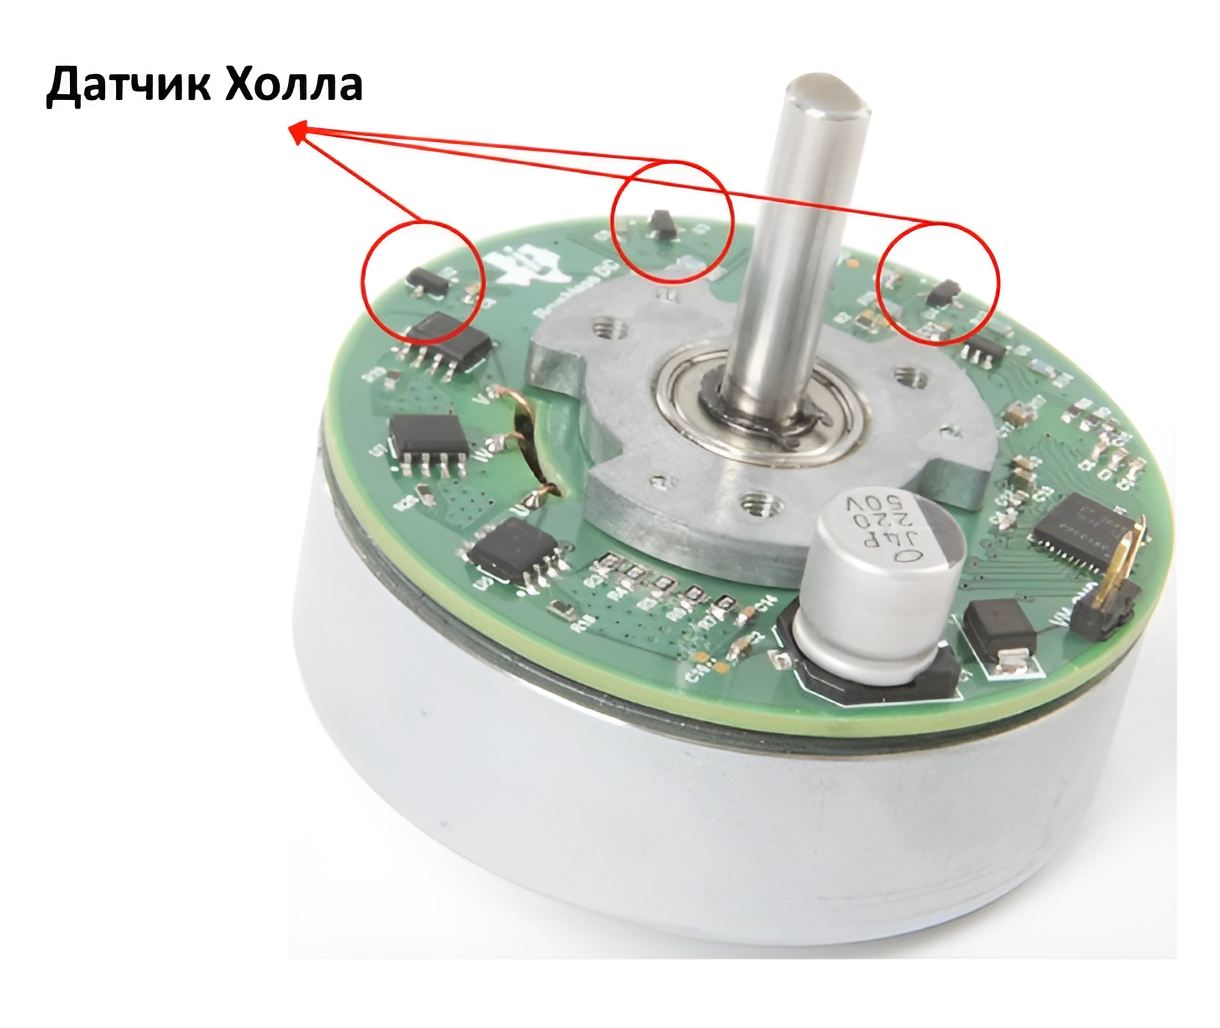
\includegraphics[width=0.7\textwidth]{inc/img/hall.png}
\caption{Возможное расположение датчиков Холла}
\end{figure}

\section{Особенности бездатчикового управления}
\label{sec:sensorless_ways}

Можно ли определить позицию ротора без использования специальных датчиков, которые удорожают конструкцию и образуют ещё один узел, который надо обслуживать, и который может выйти из строя? Для этой цели используется бесдатчиковое управление, которое сейчас набирает всё большую популярность в связи с развитием микроконтроллерной техники и увеличением производительных мощностей.

Самым популярным способом для организации такого управления является использование обратной связи по противо-ЭДС. Т. к. у нас одновременно ток протекает только через две обмотки, то на третьей обмотке индуцируется напряжение при взаимодействии с магнитным полем, по которому можно определить положение ротора. После чего можно использовать таблицу коммутации, рассмотренную в \ref{sec:hall}.

Как было отмечено в \ref{sec:bldc_theory}, противо-ЭДС в бесколлекторным двигателях имеет трапецеидальную форму, но нам это не сильно важно, ведь нужно отслеживать только точки пересечения характеристикой нуля (ZCP). Моменты переключения фаз показаны на Рисунке \ref{pic:sensorless_commut}.

\begin{figure}[!h]
\centering
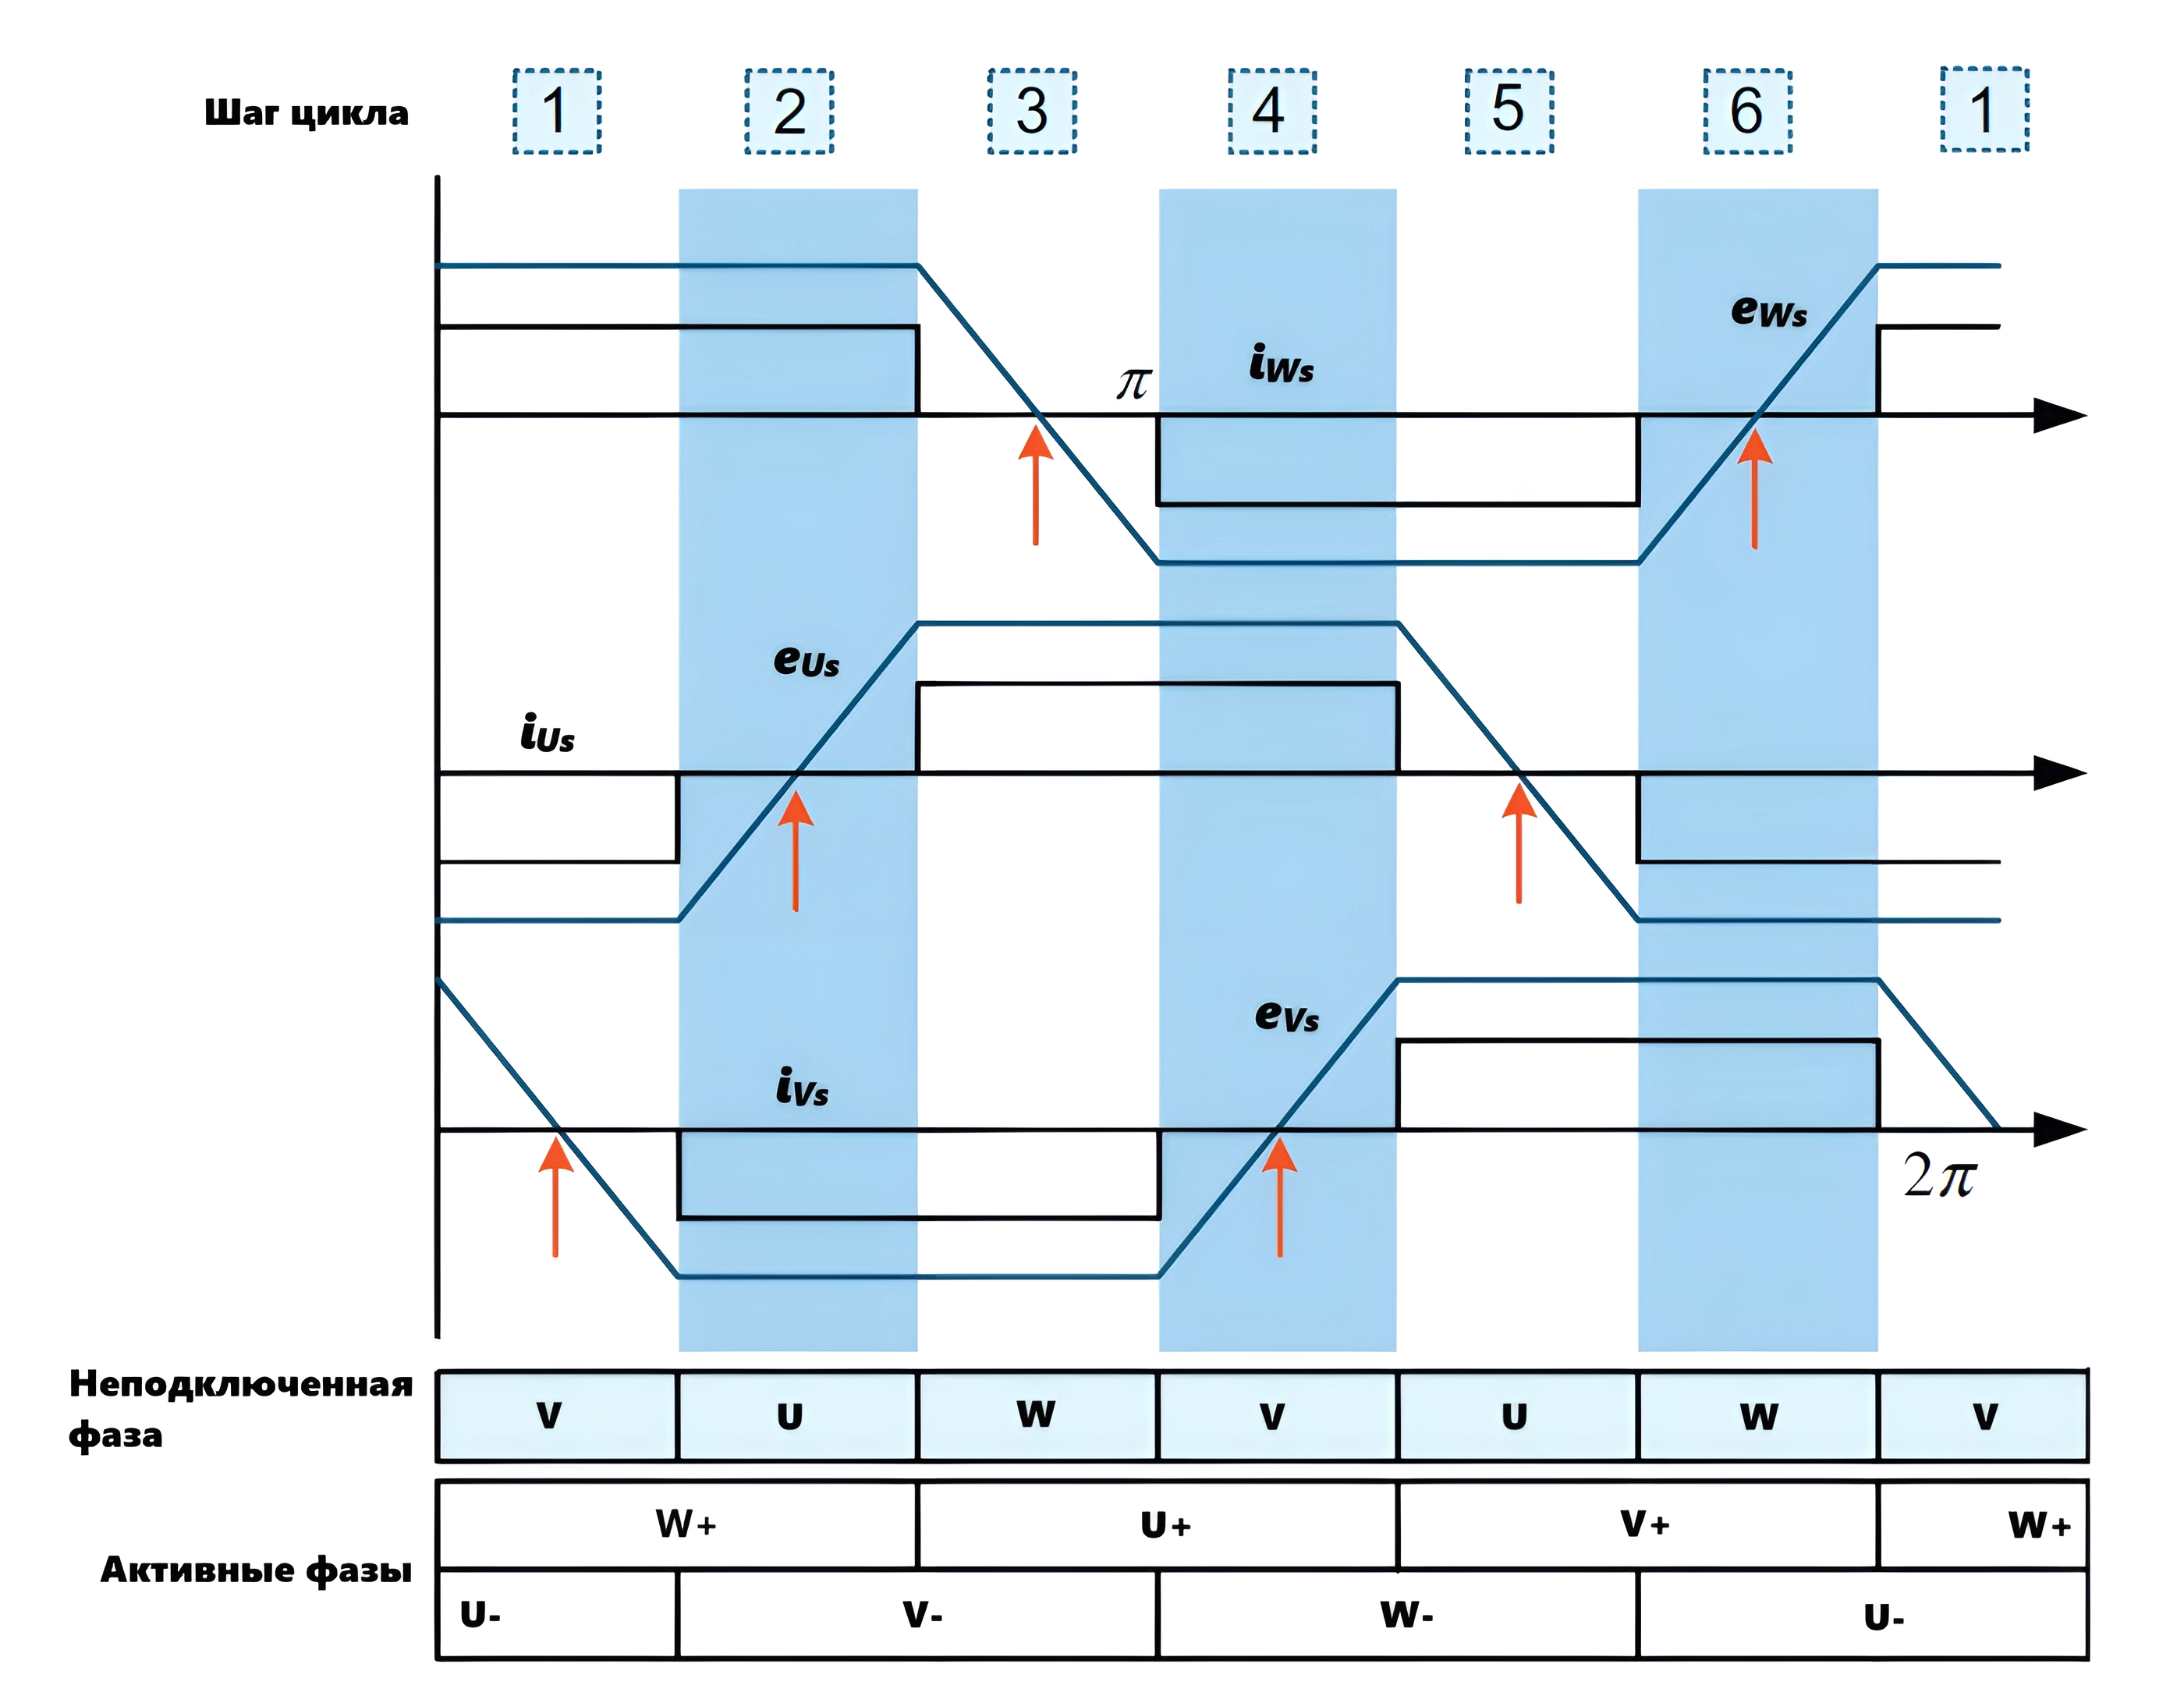
\includegraphics[width=\textwidth]{inc/img/sensorless_commut.png}
\caption{Переключение фаз в ZCP противо-ЭДС ($e$ --- противо-ЭДС фазы, $i$ --- ток фазы)}
\label{pic:sensorless_commut}
\end{figure}

Но не всё так гладко: на практике особенно на низких скоростях сложно засечь точку пересечения нуля, т. к. уменьшается амплитуда противо-ЭДС, что делает данный метод неработоспособным при необходимости управления на околонулевых скоростях, особенно в условиях шумов. В этом случае обычно цикл коммутации выполняют просто с каким-то интервалом до тех пор, пока не выйдут на скорость, достаточную для точного определения положения по противо-ЭДС.

Другие методы для определения позиции ротора без использования датчиков \cite{art:bldc_sensorless}:
\begin{enumerate}
	\item Расчёт потокосцепления из уравнения двигателя по известным величинам тока, напряжения и сопротивления ($V=Ri+\dfrac{d}{dt}\Psi$) и соотнесения его величины с позицией ротора
	\item Построение наблюдателя противо-ЭДС и последующее построение наблюдателей для положения и скорости (например, использование наблюдателя Люенбергера или наблюдателя на основе скользящих режимов)
\end{enumerate}




\chapter{Обзор алгоритмов управления скоростью}
\label{cha:chap2}

\section{ПИ (ПИД) регулятор}
\label{sec:pid}

В качестве простейшего регулятора скорости может быть использован ПИ или ПИД регулятор по скорости. Схема реализации приведена на Рисунке \ref{pic:pid1}.

\begin{figure}[!h]
\centering
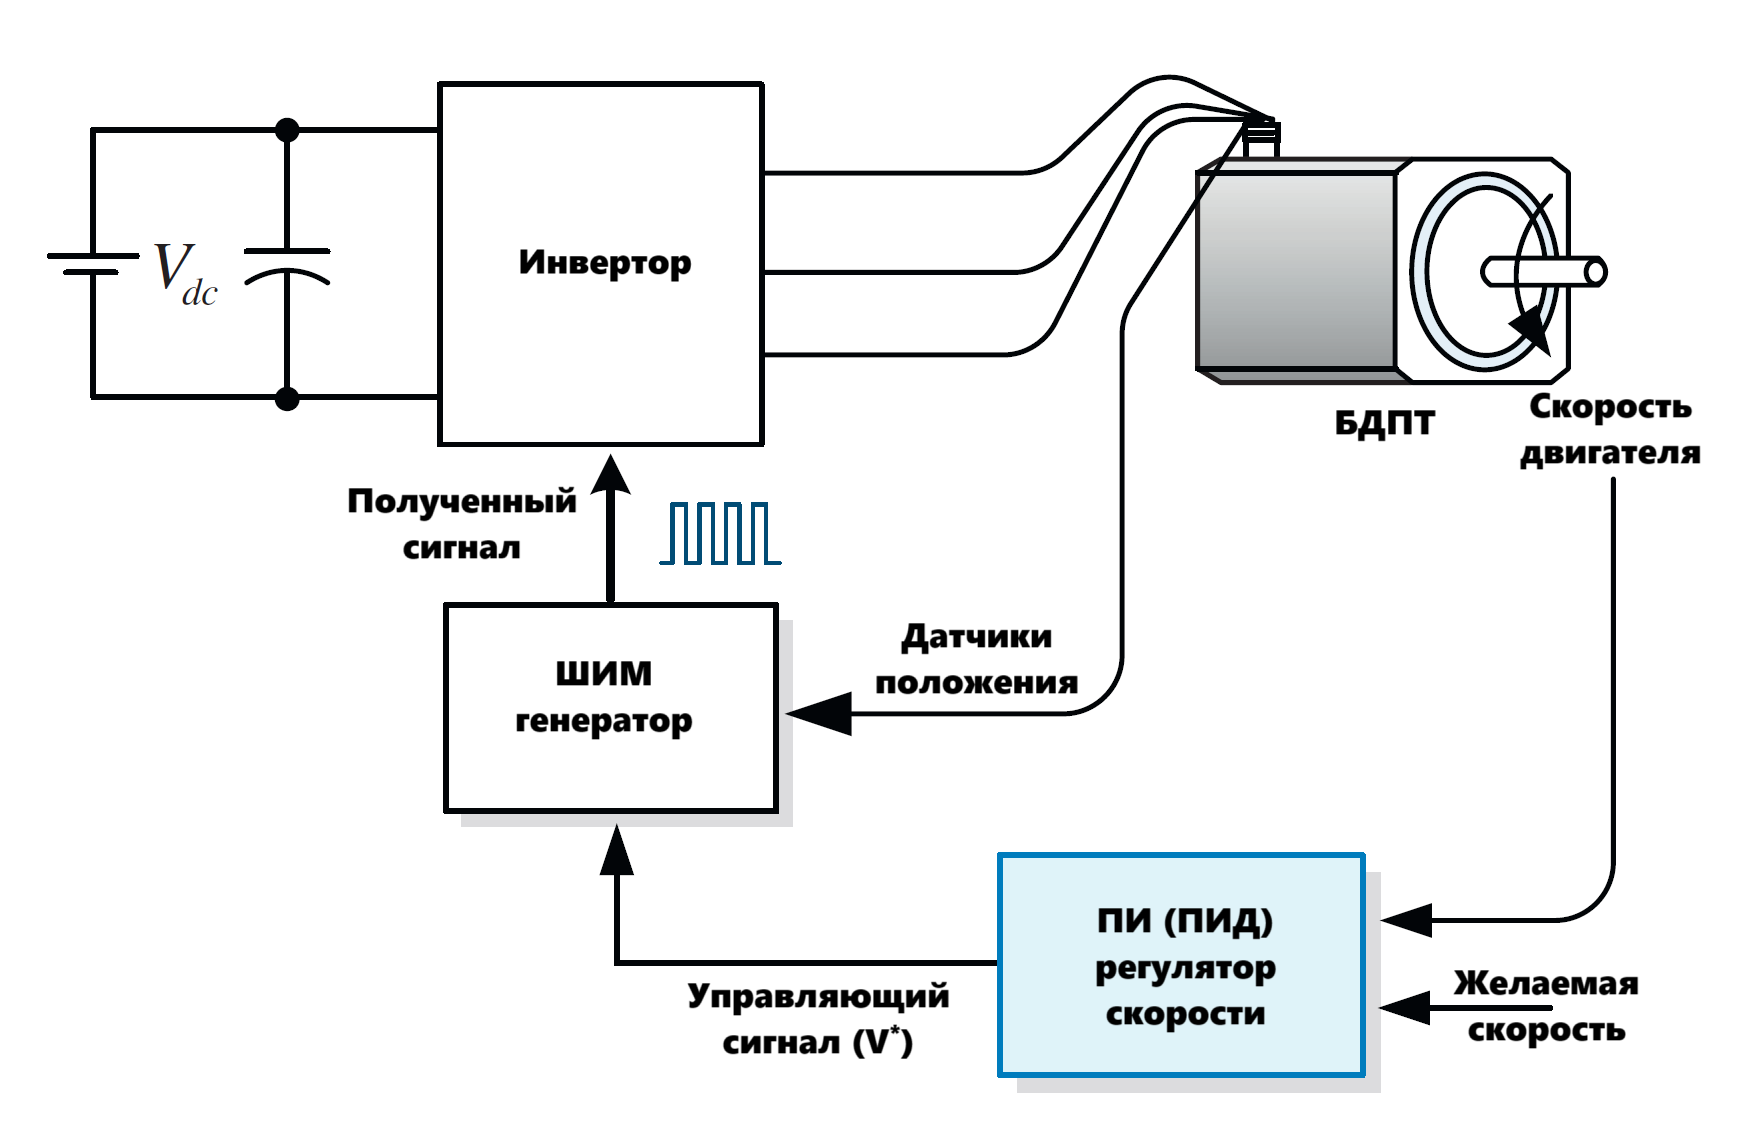
\includegraphics[width=0.7\textwidth]{inc/img/pid1.png}
\caption{Одноконтурная система регулирования скорости \cite{book.kim_motors}}
\label{pic:pid1}
\end{figure}

Данная реализация требует наличия только показаний с датчиков положения двигателя. Однако, использование системы без регулирования тока может вызвать его скачки, что может вызвать выход из строя системы, не рассчитанной на высокий ток. Для исправления этого можно добавить второй контур регулирования по току. Схема реализации приведена на Рисунке \ref{pic:pid2}.

\begin{figure}[!h]
\centering
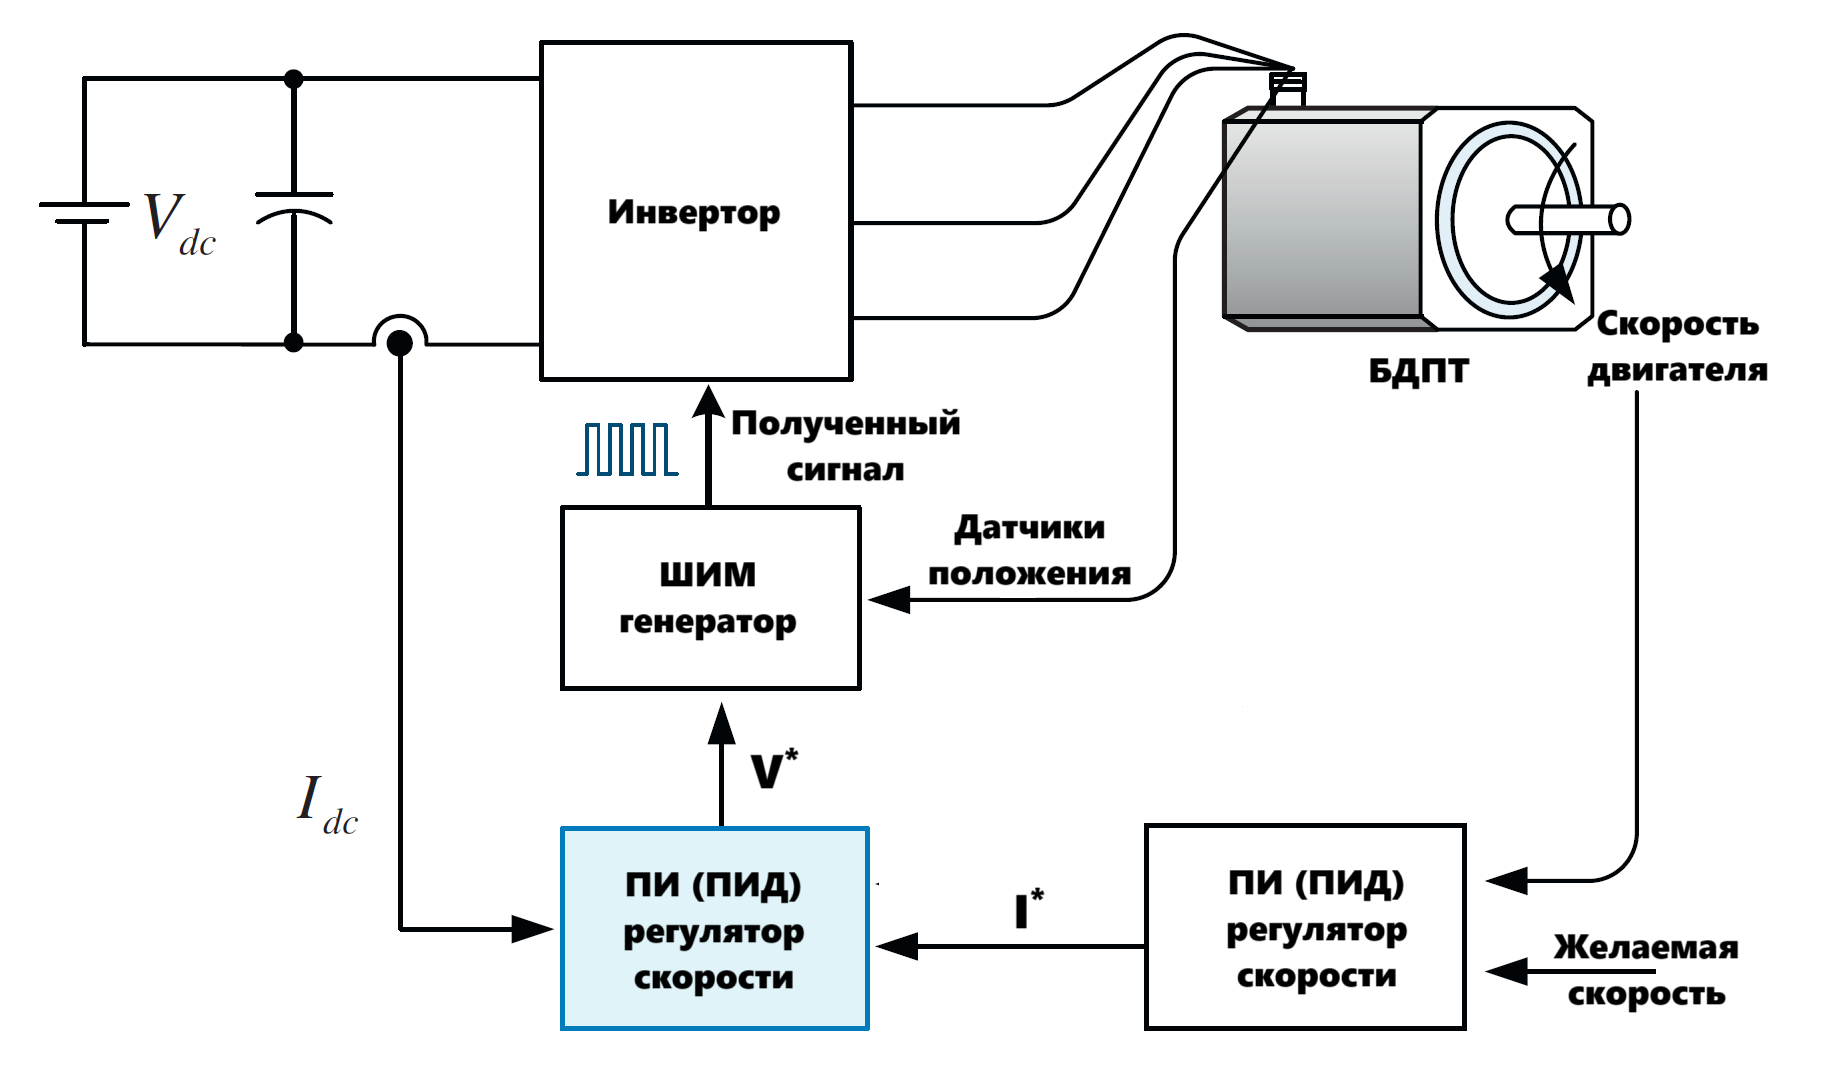
\includegraphics[width=0.7\textwidth]{inc/img/pid2.png}
\caption{Двухконтурная система регулирования скорости \cite{book.kim_motors}}
\label{pic:pid2}
\end{figure}

Для этого подхода необходимо в систему помимо датчиков положения ротора добавить датчик тока.

Использование второго контура позволяет ограничить пульсации тока во время старта и коммутации (смены питаемых обмоток), тем самым ограничив пульсации момента (ведь ток и момент связаны). Однако на практике у нас они всё равно остаются. 

Пульсации момента могут быть вызваны несколькими причинами: особенностями структуры двигателя (несинусоидальный ток и противо-ЭДС из-за питания от постоянного тока и 6-шаговой алгоритмом управления), неэффективной коммутацией во время смены фаз. Особенно сильно они заметны при переменной нагрузки. На Рисунке \ref{pic:commut} приведены графики изменения момента во время коммутации на различных скоростях.

\begin{figure}[!h]
\centering
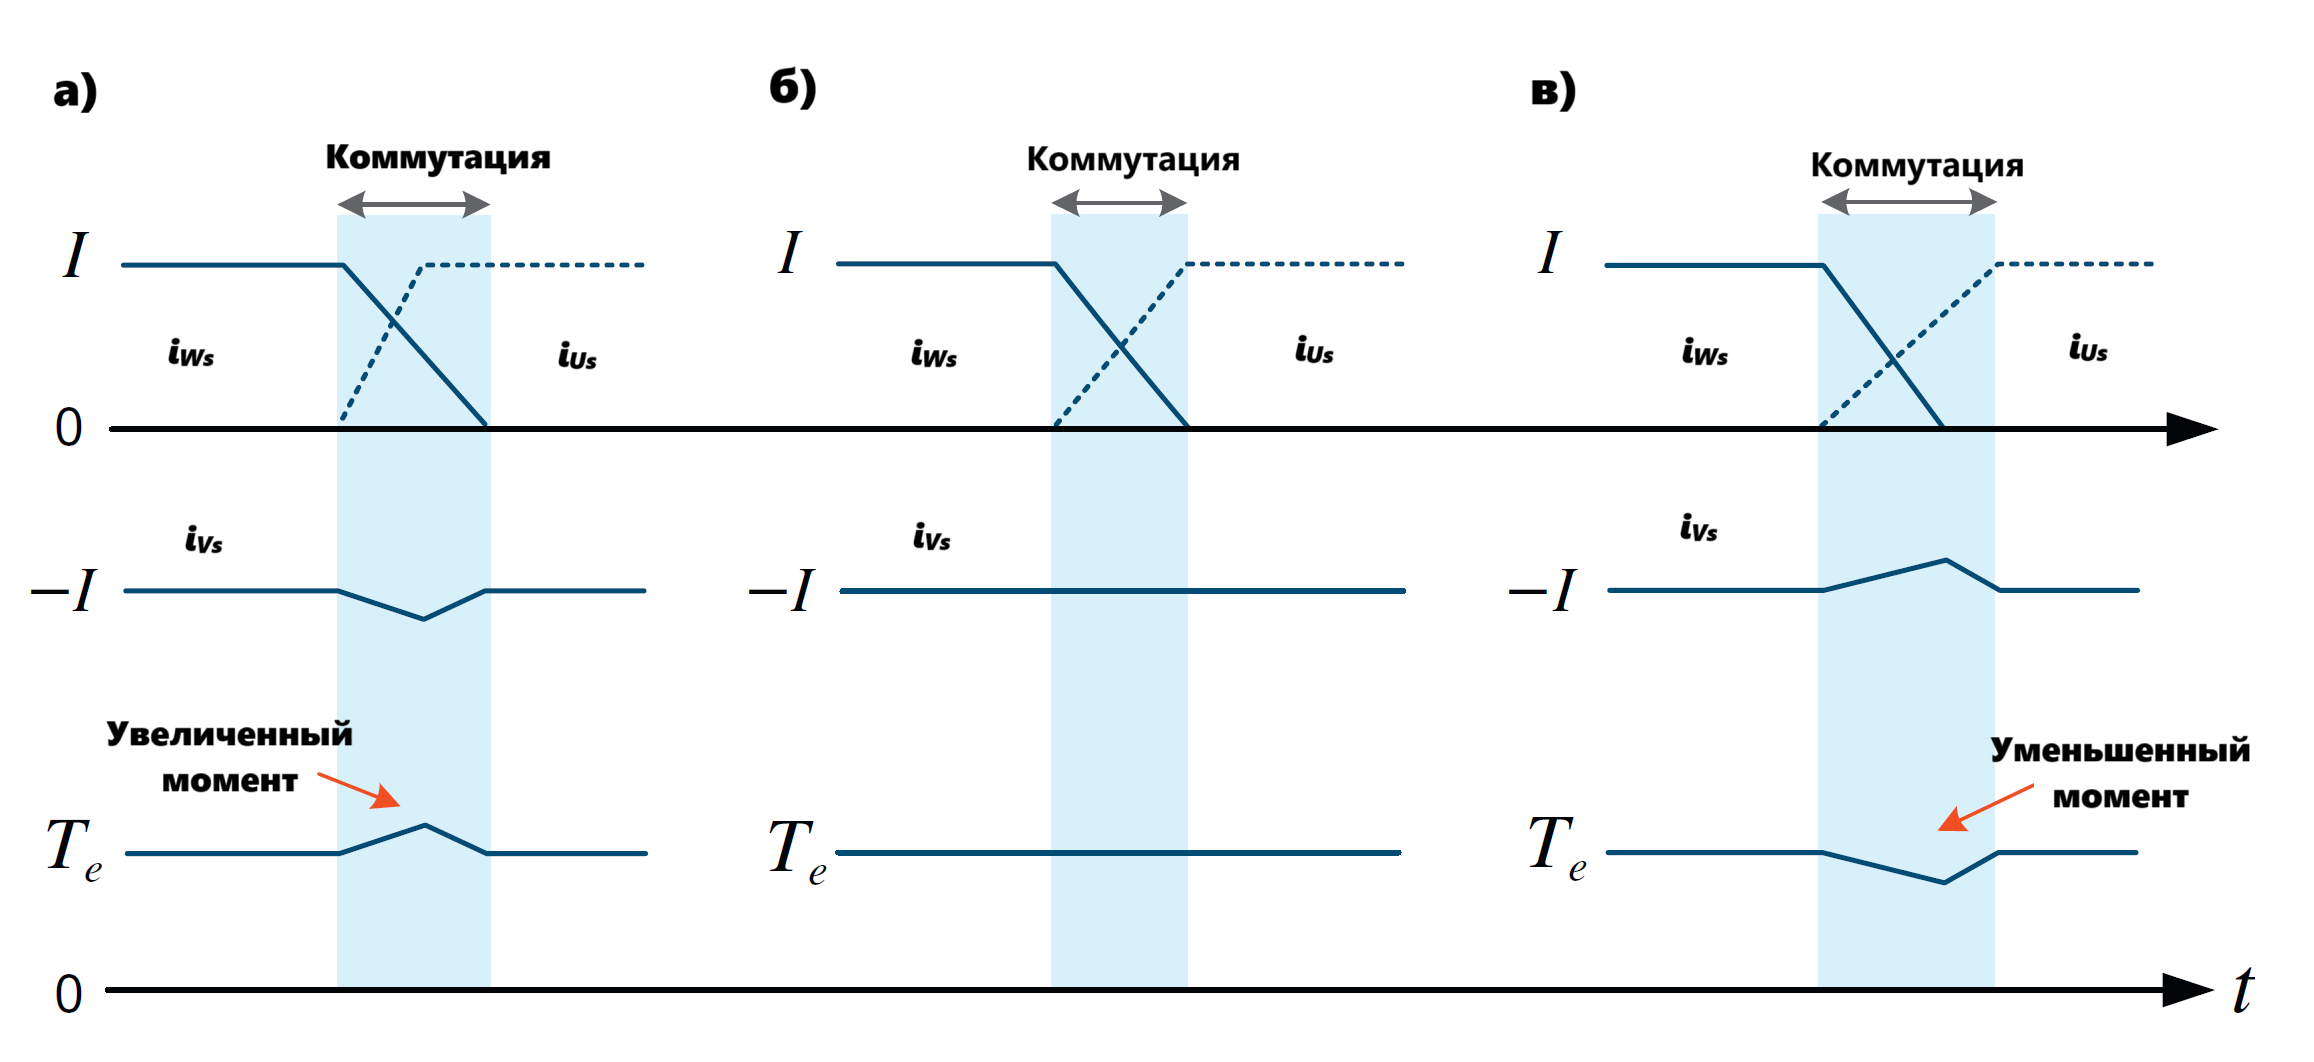
\includegraphics[width=\textwidth]{inc/img/torque_ripple.png}
\caption{Пульсации момента БДПТ на различных скоростях (а --- малые скорости ($V_{dc}>4E$), б --- средние скорости ($V_{dc}=4E$), в --- высокие скорости ($V_{dc}<4E$) ($E$ --- амплитуда противо-ЭДС)) \cite{book.kim_motors}}
\label{pic:commut}
\end{figure}

Для решения этой проблемы применяются более современные алгоритмы, рассмотренные далее.

\section{Векторное управление (FOC)}
\label{sec:foc}

Одной из самых ранних техник для уменьшения пульсаций момента является векторное управление или field orientation control (FOC). Данный алгоритм используется для независимого управления тремя параметрами двигателя (скоростью, потокосцеплением и моментом) и помогает получить форму тока статора, приближенную к синусоидальной (из-за использования синусоидального алгоритма коммутации вместо 6-шагового алгоритма), что позволяет достичь максимальный момент, располагая постоянно магнитные поля ротора и статора перпендикулярно друг другу. Возможная схема реализации этого алгоритма приведена на Рисунке \ref{pic:foc}.

\begin{figure}[!h]
\centering
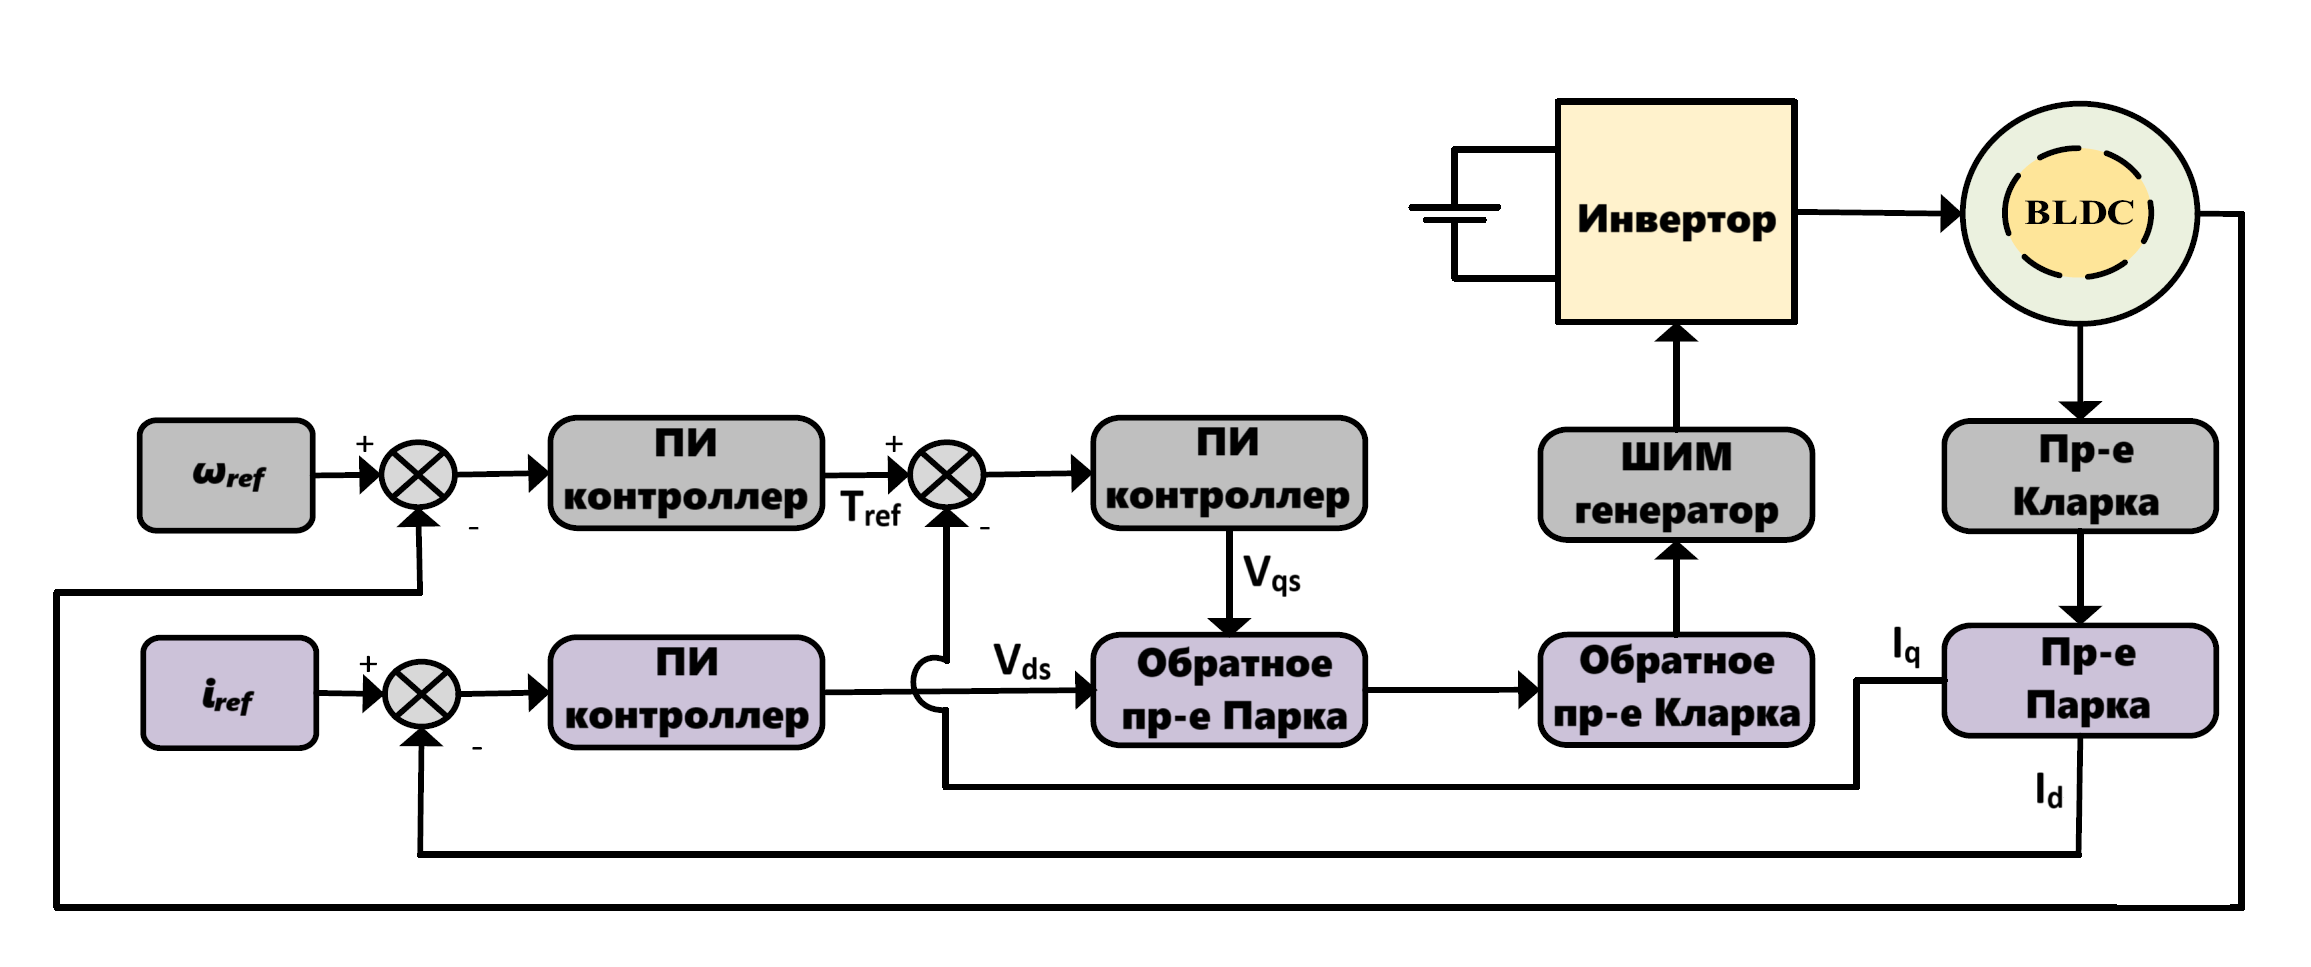
\includegraphics[width=\textwidth]{inc/img/foc.png}
\caption{Система регулирования для векторного управления ($\omega_{ref}$, $i_{ref}$ --- заданные скорость и ток регулирования; $I_d$, $I_q$ --- токи после выполнения преобразования Парка; $V_{ds}$, $V_{qs}$ --- новые векторы напряжения в $d-q$ системе координат) \cite{art:bdlc_adv_control_techs}}
\label{pic:foc}
\end{figure}

Возможный алгоритм функционирования данного типа управления \cite{art:foc_control}:
\begin{enumerate}
	\item определение токов фаз двигателя с использованием соотношения:
	\[
		i_W+i_V+i_U=0
	\]
	\item приведение трёх фазного тока к двухкоординатной системе с использованием преобразования Кларка:
	\begin{align*}
		&i_{\alpha}=i_W \\
		&i_{\beta}=(i_W+2i_V)/\sqrt{3}
	\end{align*}
	\item двухкоординатная система преобразуется для согласования с потокосцеплением ротора (вращаем для совпадения с потоком ротора на основе его угла поворота $\theta$), т. е. выполняется преобразование Парка (или преобразование во вращающуюся систему координат):
	\begin{align*}
		&I_d=i_{\alpha}\cos\theta+i_{\beta}\sin\theta\\
		&I_q=-i_{\alpha}\sin\theta+i_{\beta}\cos\theta
	\end{align*}
	\item использование полученных векторов как входов двух ПИ регуляторов для формирования на выходе векторов напряжений --- $V_{dc}$ и $V_{qs}$. $I_d$ составляющая относится к току или потокосцеплению и в качестве заданного значения используется $0$ для уменьшения пульсаций момента. $I_q$ относится к моменту. 
	\item выполнение обратного преобразования Парка:
	\begin{align*}
		&V_{\alpha}=V_{dc}\cos\theta-V_{qs}\sin\theta \\
		&V_{\beta}=V_{dc}\sin\theta+V_{qs}\cos\theta
	\end{align*}
	\item выполнение обратного преобразования Кларка:
	\begin{align*}
		&V_W=V_{\beta}\\
		&V_V=(-V_{\beta}+\sqrt{3}V_{\alpha})/2\\
		&V_U=(-V_{\beta}-\sqrt{3}V_{\alpha})/2
	\end{align*}
	\item полученные напряжения используются для генерации ШИМ сигнала на основе алгоритма SVPWM (пространственно-векторная широтно-импульсная модуляции) или SPWM (синусоидальная широтно-импульсная модуляция).
\end{enumerate}

Хоть данный метод и позволяет уменьшить пульсации момента, но для его нормального функционирования необходимо наличие датчиков положения ротора. Конечно, можно управлять и бездатчиковым методом, но обычно это выполняется с использованием наблюдателей положения и скорости на основе оценки противо-ЭДС, что требует больше вычислительных мощностей, больше информации о двигателе и является менее надёжным.

\section{Прямое управление моментом (DTC)}

В основе данного метода лежит оценка электромагнитного момента на основе тока и напряжения фаз статора и электрического положения ротора, и его последующее регулирование. Возможная схема реализации этого алгоритма приведена на Рисунке \ref{pic:dtc}.

\begin{figure}[!h]
\centering
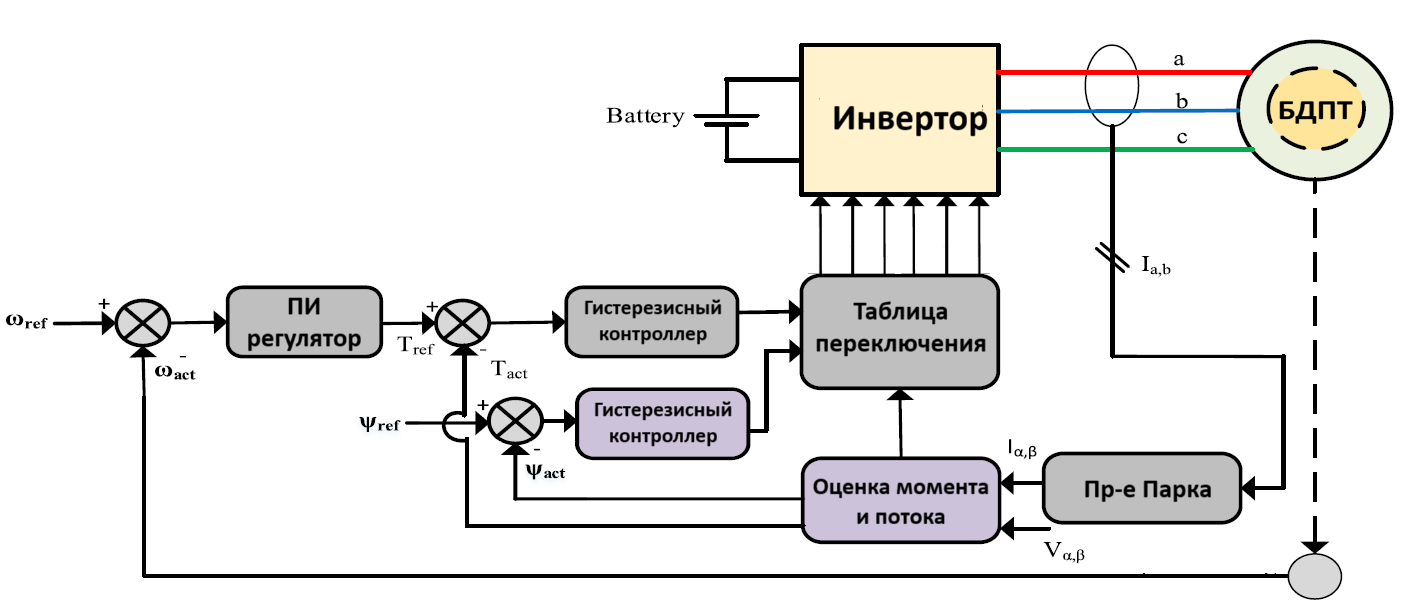
\includegraphics[width=\textwidth]{inc/img/dtc.png}
\caption{Система регулирования для прямого управления моментом ($\omega_{m(ref)}$, $M_{e(ref)}$ --- заданные скорость и момент регулирования; $\omega_{m(act)}$, $\omega_{e(hat)}$ --- текущая скорость и оценка момента; $I_{\alpha\beta}$, $V_{\alpha\beta}$ --- токи и напряжения после выполнения преобразования Кларка) \cite{art:bdlc_adv_control_techs}}
\label{pic:dtc}
\end{figure}

Возможный алгоритм работы следующий:
\begin{enumerate}
	\item выполнить переход к двумерной системе координат для тока и напряжения фаз путём выполнения преобразования Кларка, определить угол положения ротора в электрических градусах;
	\item оценить на основе полученных данных электромагнитный момент двигателя;
	\item получить ошибки по моменту, взяв за желаемое значение выход ПИ регулятора контура скорости;
	\item пропустить ошибки через ПИ или гистерезисные контроллеры (последние представляют в самом простом случае функцию переключения с гистерезисом, которые на выходе имеют $1$ при превышении верхнего порога и $-1$ при выхода за нижний порог);
	\item на основе полученных значений выходов и текущего положения ротора получить новые состояния ключей инвертора согласно специальной таблице коммутации.
\end{enumerate}

Данный метод является менее требовательным в плане вычислительных мощностей, обладает большей робастностью по отношению к параметрам двигателя и обладает лучшими динамическими свойствами по сравнению с векторным управлением. Однако для его нормального функционирования необходима большая частота работы регулятора (большой период дискретизации), особенно при использовании гистерезисных регуляторов, отчего зависят напрямую амплитуды пульсаций момента и скорости. Также он обладает меньшей эффективностью по сравнению с векторным управлением, но при этом его простота позволяет просто реализовать и настроить (нужно лишь найти подходящие параметры ПИ регуляторов и/или выставить пороги гистерезисных регуляторов).
\chapter{Разрабатываемое техническое решение}
\label{cha:chap3}

\section{Определение принципа работы двигателя и выбор алгоритма управления}

Для исследования был выбран двигатель без установленных датчиков Холла, поэтому необходимо использовать один из приёмов определения положения ротора, рассмотренных в \ref{sec:sensorless_ways}. Был выбран метод на основе наблюдателя противо-ЭДС, из которого можно получить положение ротора и скорость.

Что касается выбора алгоритма управления скоростью, то предпочтение отдаётся методу на основе прямого управления моментом в силу его простоты, робастности и меньшей вычислительной нагрузки по сравнению с другими рассмотренными методами.

Из-за того, что выбранный алгоритм не так ресурсозатратен, нежели другой метод на основе прямого управления моментом --- векторное управление, в условиях ограниченных вычислительных ресурсов можно позволить увеличить частоту измерений и расчётов, что также положительно скажется на динамических свойствах и позволит увеличить точность регулирования.

\section{Необходимые узлы для реализации технического решения}
\label{sec:nodes}

На основе выбранных принципов функционирования устройства и алгоритма управления система должна включать в себя следующие узлы:
\begin{enumerate}
	\item блок с логикой управления;
	\item инвертор, служащий для преобразования ШИМ сигнала и сигнала с системы регулирования в сигналы для управления фазами двигателя;
	\item механизм определения тока и напряжения фаз для функционирования алгоритма;
	\item блок питания двигателя;
	\item БДПТ без установленных датчиков положения.
\end{enumerate}

\chapter{Проектирование модели системы}
\label{cha:chap4}

\section{Математическая модель двигателя}

Трёх фазный БДПТ может быть описан следующей системой уравнений\cite{art:dtc_smo}: 
\begin{align}
\label{sys:abc}
\left\{ \begin{aligned} 
  v_{ab}=R_si_{ab}+L_s\dfrac{d}{dt}i_{ab}+e_{ab}\\
  v_{bc}=R_si_{bc}+L_s\dfrac{d}{dt}i_{bc}+e_{bc}\\
  v_{ca}=R_si_{ca}+L_s\dfrac{d}{dt}i_{ca}+e_{ca}
\end{aligned} \right.
\end{align}, где $a$, $b$, $c$ --- фазы двигателя; $v_{ab}$, $v_{bc}$, $v_{ca}$ --- напряжения между соответствующими фазами; $i_{ab}$, $i_{bc}$, $i_{ca}$ --- разница токов соответствующих фаз; $e_{ab}$, $e_{bc}$, $e_{ca}$ --- противо-ЭДС между соответствующими фазами; $R_s$ --- сопротивление статора; $L_s$ --- индуктивность статора

Уравнение динамики описывается следующим образом:
\begin{align*}
	T_e = T_L+B\omega_m+J\dfrac{d\omega_m}{dt}
\end{align*}, где $T_e$ --- электромагнитный момент; $T_L$ --- момент нагрузки; $B$ --- коэффициент трения; $J$ --- момент инерции ротора; $\omega_m$ --- механический момент ротора

Противо-ЭДС может быть выражена следующей зависимостью от скорости:
\begin{align*}
	e_{abc}=k_e\omega_m
\end{align*}, где $k_e$ --- постоянная по противо-ЭДС

\section{Наблюдатель скользящего режима (SMO)}
\label{sec:smo}

Т. к. у нас двигатель без установленных датчиков положения, то нам необходимо его оценивать для реализации алгоритма управления. Можно рассмотреть классический наблюдатель Люенбергера \cite{art:obs_luen_bldc}, но его устойчивость сильно зависит от параметров, используемых при построении, что не подходит под требования технического задания. Поэтому был выбран наблюдатель на основе скользящего режима, т. к. он работает при вариации параметров двигателя во время работы, т. е. обладает большей рабостностью. Также он требует меньше вычислительных мощностей, что позволяет увеличить частоту измерений.

Для удобства дальнейших расчётов запишем \ref{sys:abc} в двумерной $\alpha-\beta$ системе:
\begin{align}
\label{sys:albet}
\left\{ \begin{aligned} 
  &v_{\alpha}=R_si_{\alpha}+L_s\dfrac{d}{dt}i_{\alpha}+e_{\alpha}\\
  &v_{\beta}=R_si_{\beta}+L_s\dfrac{d}{dt}i_{\beta}+e_{\beta}
\end{aligned} \right.
\end{align}

Или в матричной форме: \cite{art:smo}
\begin{align}
\label{sys:albetmat}
\dot{i}_{\alpha\beta}=\Phi i_{\alpha\beta}+\Gamma v_{\alpha\beta}-\Gamma e_{\alpha\beta}
\end{align}, где $i_{\alpha\beta}=\begin{bmatrix}
	i_{\alpha} & i_{\beta}
\end{bmatrix}$, $v_{\alpha\beta}=\begin{bmatrix}
	v_{\alpha} & v_{\beta}
\end{bmatrix}$, $e_{\alpha\beta}=\begin{bmatrix}
	e_{\alpha} & e_{\beta}
\end{bmatrix}$, $\Phi=\begin{bmatrix}
	-R_s/L_s & 0 \\
	0 & -R_s/L_s
\end{bmatrix}$, $\Gamma = \begin{bmatrix}
	1/L_s & 0 \\
	0 & 1/L_s
\end{bmatrix}$

Также поведение противо-ЭДС может быть представлено в следующей форме:
\begin{align}
\label{e_albet}
	\dot{e}_{\alpha\beta}=\omega_eJe_{\alpha\beta}
\end{align}, где $\omega_e$ --- электрическая скорость двигателя ($\omega_e=\omega_m\cdot p$ ($p$ --- количество пар полюсов двигателя)); $J=\begin{bmatrix}
 0 & -1 \\
 1 & 0
\end{bmatrix}$

Рассмотрим дискретный наблюдатель, рассмотренный в \cite{art:smo}. Для этого рассмотрим \ref{sys:albetmat} и \ref{e_albet} в дискретной форме:
\begin{align}
	&i_{\alpha\beta(k+1)}=Ai_{\alpha\beta(k)}+Bv_{\alpha\beta(k)}-Be_{\alpha\beta(k)}\\
	&e_{\alpha\beta(k+1)}=e_{\alpha\beta(k)}+T_s\omega_{e(k)}Je_{\alpha\beta(k)}
\end{align}, где $T_s$ --- период дискретизации; $A=e^{\Phi T_s}$; $B=\int_0^{T_s}e^{\Phi\tau}\Gamma d\tau=\begin{bmatrix}
	b & 0 \\
	0 & b
\end{bmatrix}$ $\left(b=\dfrac{1-e^{-R_sT_s/L_s}}{R_s}\right)$

Тогда наблюдатель на основе скользящего режима задаётся следующими уравнениями:
\begin{align}
	&\hat{i}_{\alpha\beta(k+1)}=A\hat{i}_{\alpha\beta(k)}+Bv_{\alpha\beta(k)}-B\hat{e}_{\alpha\beta(k)}-\eta sign(\tilde{i}_{\alpha\beta(k)})\\
	\label{eq:hat_e}
	&\hat{e}_{\alpha\beta(k+1)}=\hat{e}_{\alpha\beta(k)}+B^{-1}g(\tilde{i}_{\alpha\beta(k)}-A\tilde{i}_{\alpha\beta(k-1)}+\eta sign(\tilde{i}_{\alpha\beta(k-1)}))\\
	&\tilde{i}_{\alpha\beta(k)}=\hat{i}_{\alpha\beta(k)}-i_{\alpha\beta(k)}\\
	&\tilde{e}_{\alpha\beta(k)}=\hat{e_{\alpha\beta(k)}}-e_{\alpha\beta(k)}
\end{align}, где $\eta$ --- коэффициент усиления по противо-ЭДС; $g$ --- коэффициент усиления по току

Выбор коэффициентов осуществляется из следующих условий:
\begin{enumerate}
	\item Если $|e_{\alpha\beta(k+1)}-e_{\alpha\beta(k)}|\leq m$ и коэффициент $g\in (0, 1)$ тогда существует $k_0$ такое, что при $k\geq k_0$ выполняется:
	\begin{align*}
		\tilde{e}_{\alpha\beta(k)}<\dfrac{m}{g}
	\end{align*}
	\item Если $|e_{\alpha\beta(k+1)}-e_{\alpha\beta(k)}|\leq m$, коэффициент $g\in (0, 1)$ и $\eta>b\dfrac{m}{g}$ тогда существует $k_0$ такое, что при $k\geq k_0$ выполняется:
	\begin{align*}
		|\tilde{i}_{\alpha\beta(k)}|\leq \eta +b\dfrac{m}{g}
	\end{align*}
\end{enumerate}

Таким образом, при правильном выборе параметров наблюдателя обеспечивается ограниченность векторов невязки по противо-ЭДС и току.

Главным недостатком такого вида наблюдателя, как и любых систем на основе скользящих режимов, является чаттеринг (дребезг) при приближении к поверхности скольжения, что уменьшает точность регулирования и увеличивает частоту перключений фаз, внося дополнительные потери и понижая срок службы электрических компонентов. Для уменьшения его амплитуды может применяться фильтр нижних частот на выходе оценок противо-ЭДС \cite{art:smo} и/или замена функций знакового переключения на функции переключения с насыщением \cite{art:dtc_smo}.

Оценка электрического положение ротора может быть найдено из \ref{eq:hat_e} по следующей формуле:
\begin{align*}
	\hat{\theta}_e = \tan^{-1}\left(-\dfrac{\hat{e_\alpha}}{\hat{e_\beta}}\right)
\end{align*}

Из чего можно найти скорость вращения ротора, зная число пар полюсов двигателя ($p$).

\section{Прямое управление моментом}

Для реализации этого алгоритма управления необходимо знание электромагнитного момента ($T_e$), который может быть найден следующим образом\cite{art:dtc_smo}:  
\begin{align}
	\label{Te}
	&T_e=\dfrac{3p}{4}\left(\dfrac{d\Psi_{r\alpha}}{d\theta_e}i_{\alpha}+\dfrac{d\Psi_{r\beta}}{d\theta_e}i_{\beta}\right)
\end{align}, где $\Psi_{r\alpha}$, $\Psi_{r\beta}$ --- поток статора в $\alpha-\beta$ координатах.

Производные потока ротора от электрического положения ротора могут быть представлены следующими соотношениями:
\begin{align}
	\label{psira}
	&\dfrac{d\Psi_{r\alpha}}{d\theta_e}=\dfrac{d\Psi_{r\alpha}}{dt}\dfrac{dt}{d\theta_e}=\dfrac{1}{\omega_e}\dfrac{d\Psi_{r\alpha}}{dt}=\dfrac{e_\alpha}{\omega_e}\\
	&\dfrac{d\Psi_{r\beta}}{d\theta_e}=\dfrac{d\Psi_{r\beta}}{dt}\dfrac{dt}{d\theta_e}=\dfrac{1}{\omega_e}\dfrac{d\Psi_{r\beta}}{dt}=\dfrac{e_\beta}{\omega_e}
\end{align}

С учётом \ref{psira} и \ref{Te} можем получить:
\begin{align*}
	T_e=\dfrac{3p}{4}\left(\dfrac{e_{\alpha}}{\omega_e}i_{\alpha}+\dfrac{e_{\beta}}{\omega_e}i_{\beta}\right)
\end{align*}

Из этого уравнения и оценки противо-ЭДС рассчитывается значения оценки электромагнитного момента:
\begin{align}
\label{eq:T_e}
	&\hat{T}_e=\dfrac{3p}{4}\left(\dfrac{\hat{e}_{\alpha}}{\omega_e}i_{\alpha}+\dfrac{\hat{e}_{\beta}}{\omega_e}i_{\beta}\right)=\dfrac{3}{4}\left(\dfrac{\hat{e}_{\alpha}}{\omega_m}i_{\alpha}+\dfrac{\hat{e}_{\beta}}{\omega_m}i_{\beta}\right)
\end{align}

В нашей системе мы будем управлять только моментом, не затрагивая управление потоком для уменьшения вычислительных затрат и возможности дополнительно повысить период дискретизации.

\section{Модель системы в Simulink}

На основе математических формул, приведённых выше, была построена модель системы, приведённая на рисунке \ref{pic:mod1}.

\begin{figure}[!h]
\centering
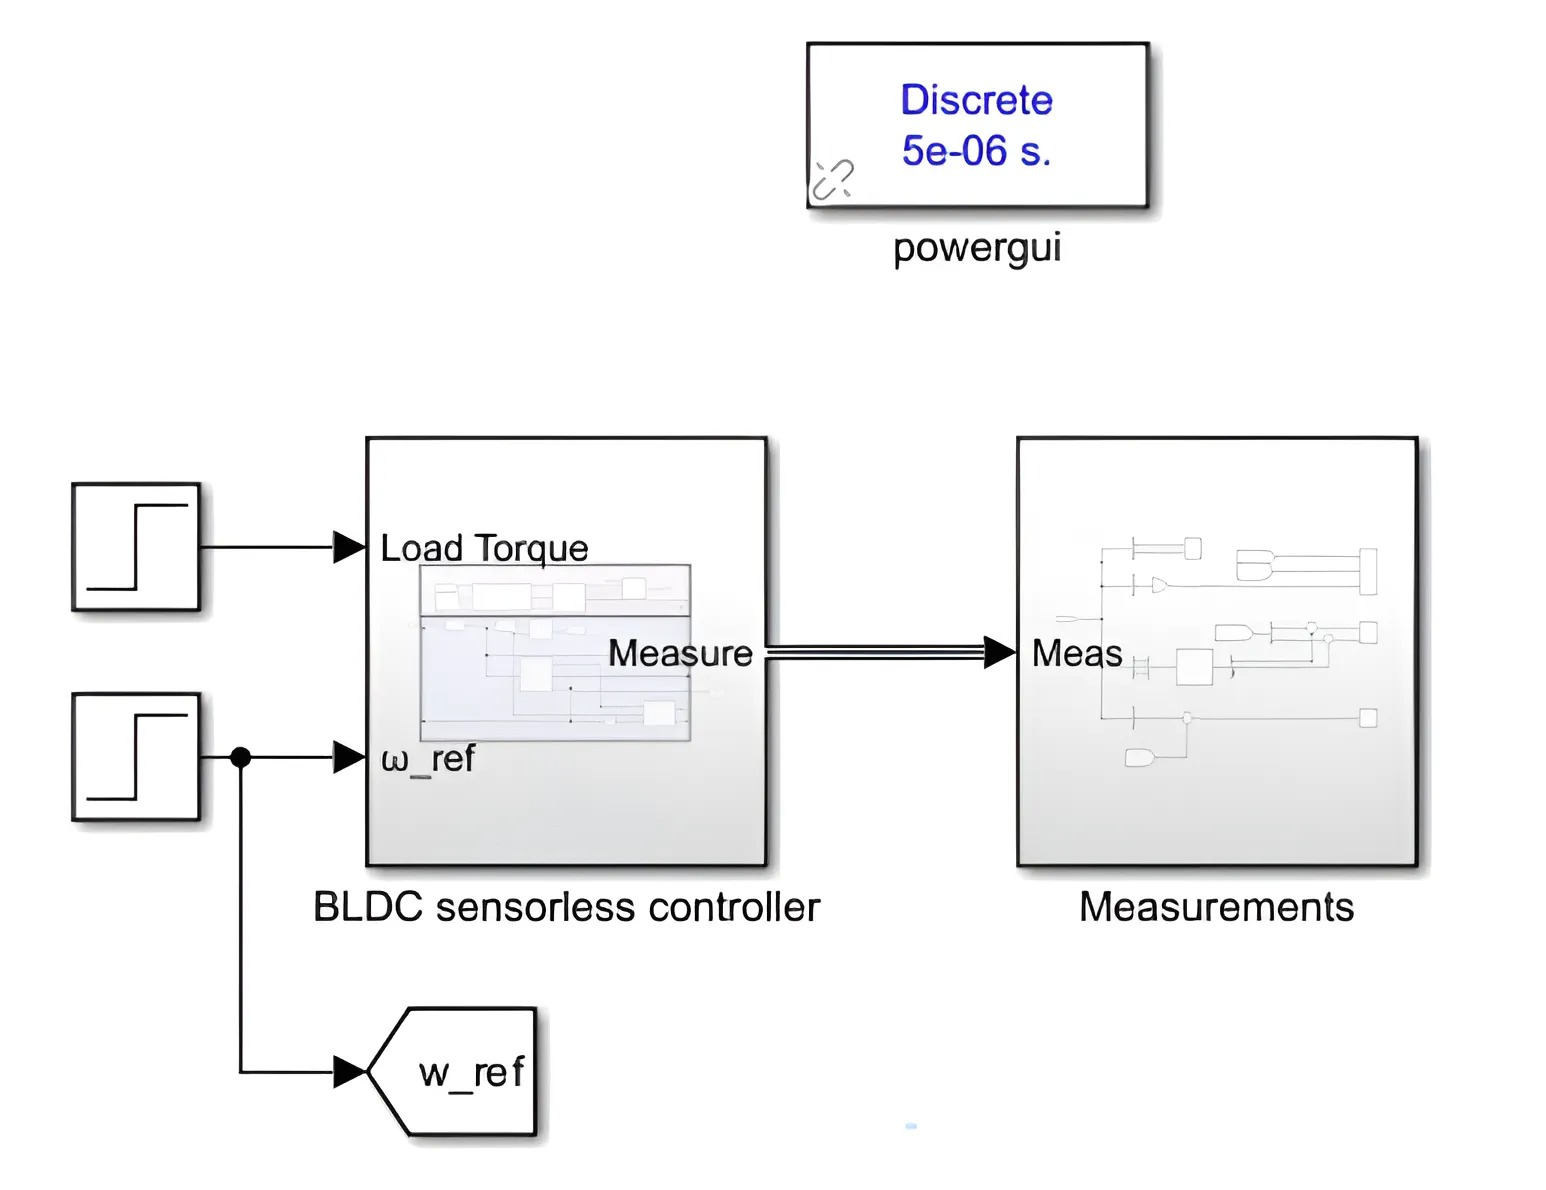
\includegraphics[width=0.7\textwidth]{inc/img/model1.png}
\caption{Общая модель системы}
\label{pic:mod1}
\end{figure}

Она состоит из двух основных блоков. Первый из них приведён на рисунке \ref{pic:mod2} и содержит силовую часть из инвертора, двигателя и источника питания, систему управления, которая представляет из себя двухконтурный регулятор (первый контур по скорости, второй по моменту). Электромагнитный момент находится по формуле \ref{eq:T_e} на основе параметров, получаемых при оценке с помощью наблюдателя скользящего режима, описанного в \ref{sec:smo}.

\begin{figure}[!h]
\centering
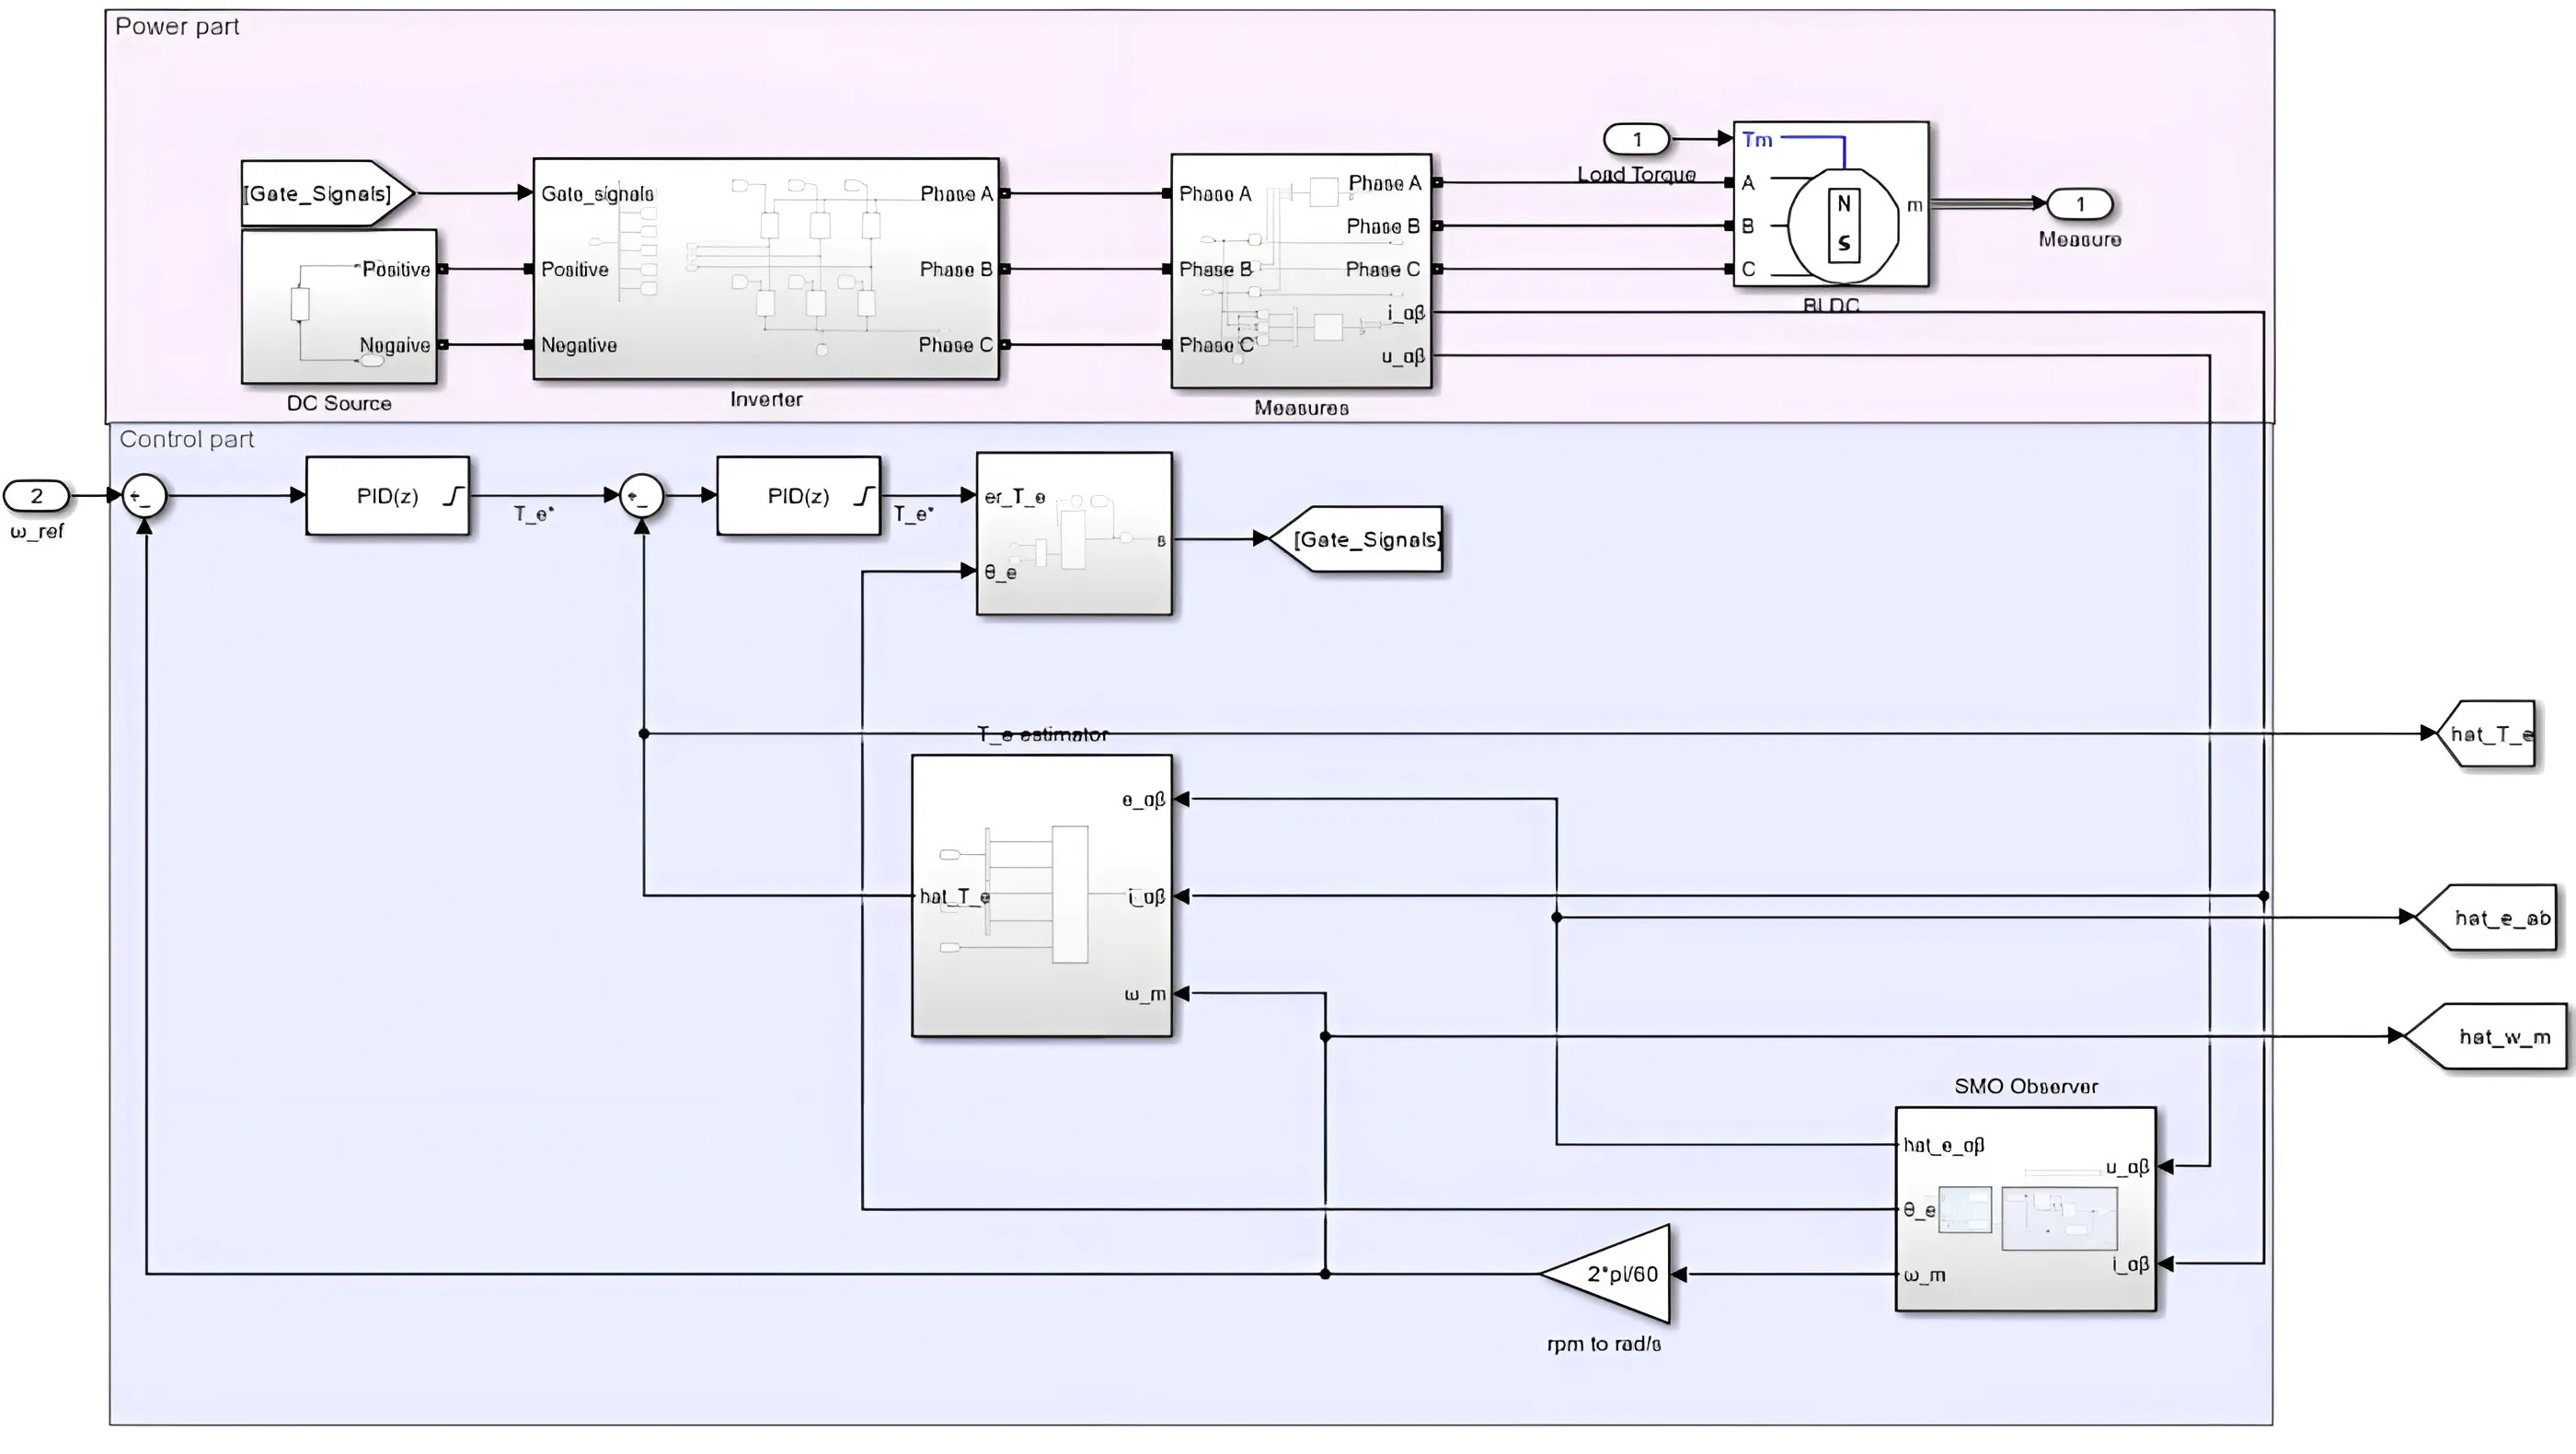
\includegraphics[width=1\textwidth]{inc/img/model2.png}
\caption{Блок с системой управления и силовой частью}
\label{pic:mod2}
\end{figure}

Инвертор представляет собой 6 ключей на основе Mosfet транзисторов (Рисунок \ref{pic:mod4}) и питается от источника постоянного напряжения (Рисунок \ref{pic:mod3})

\begin{figure}[!h]
\centering
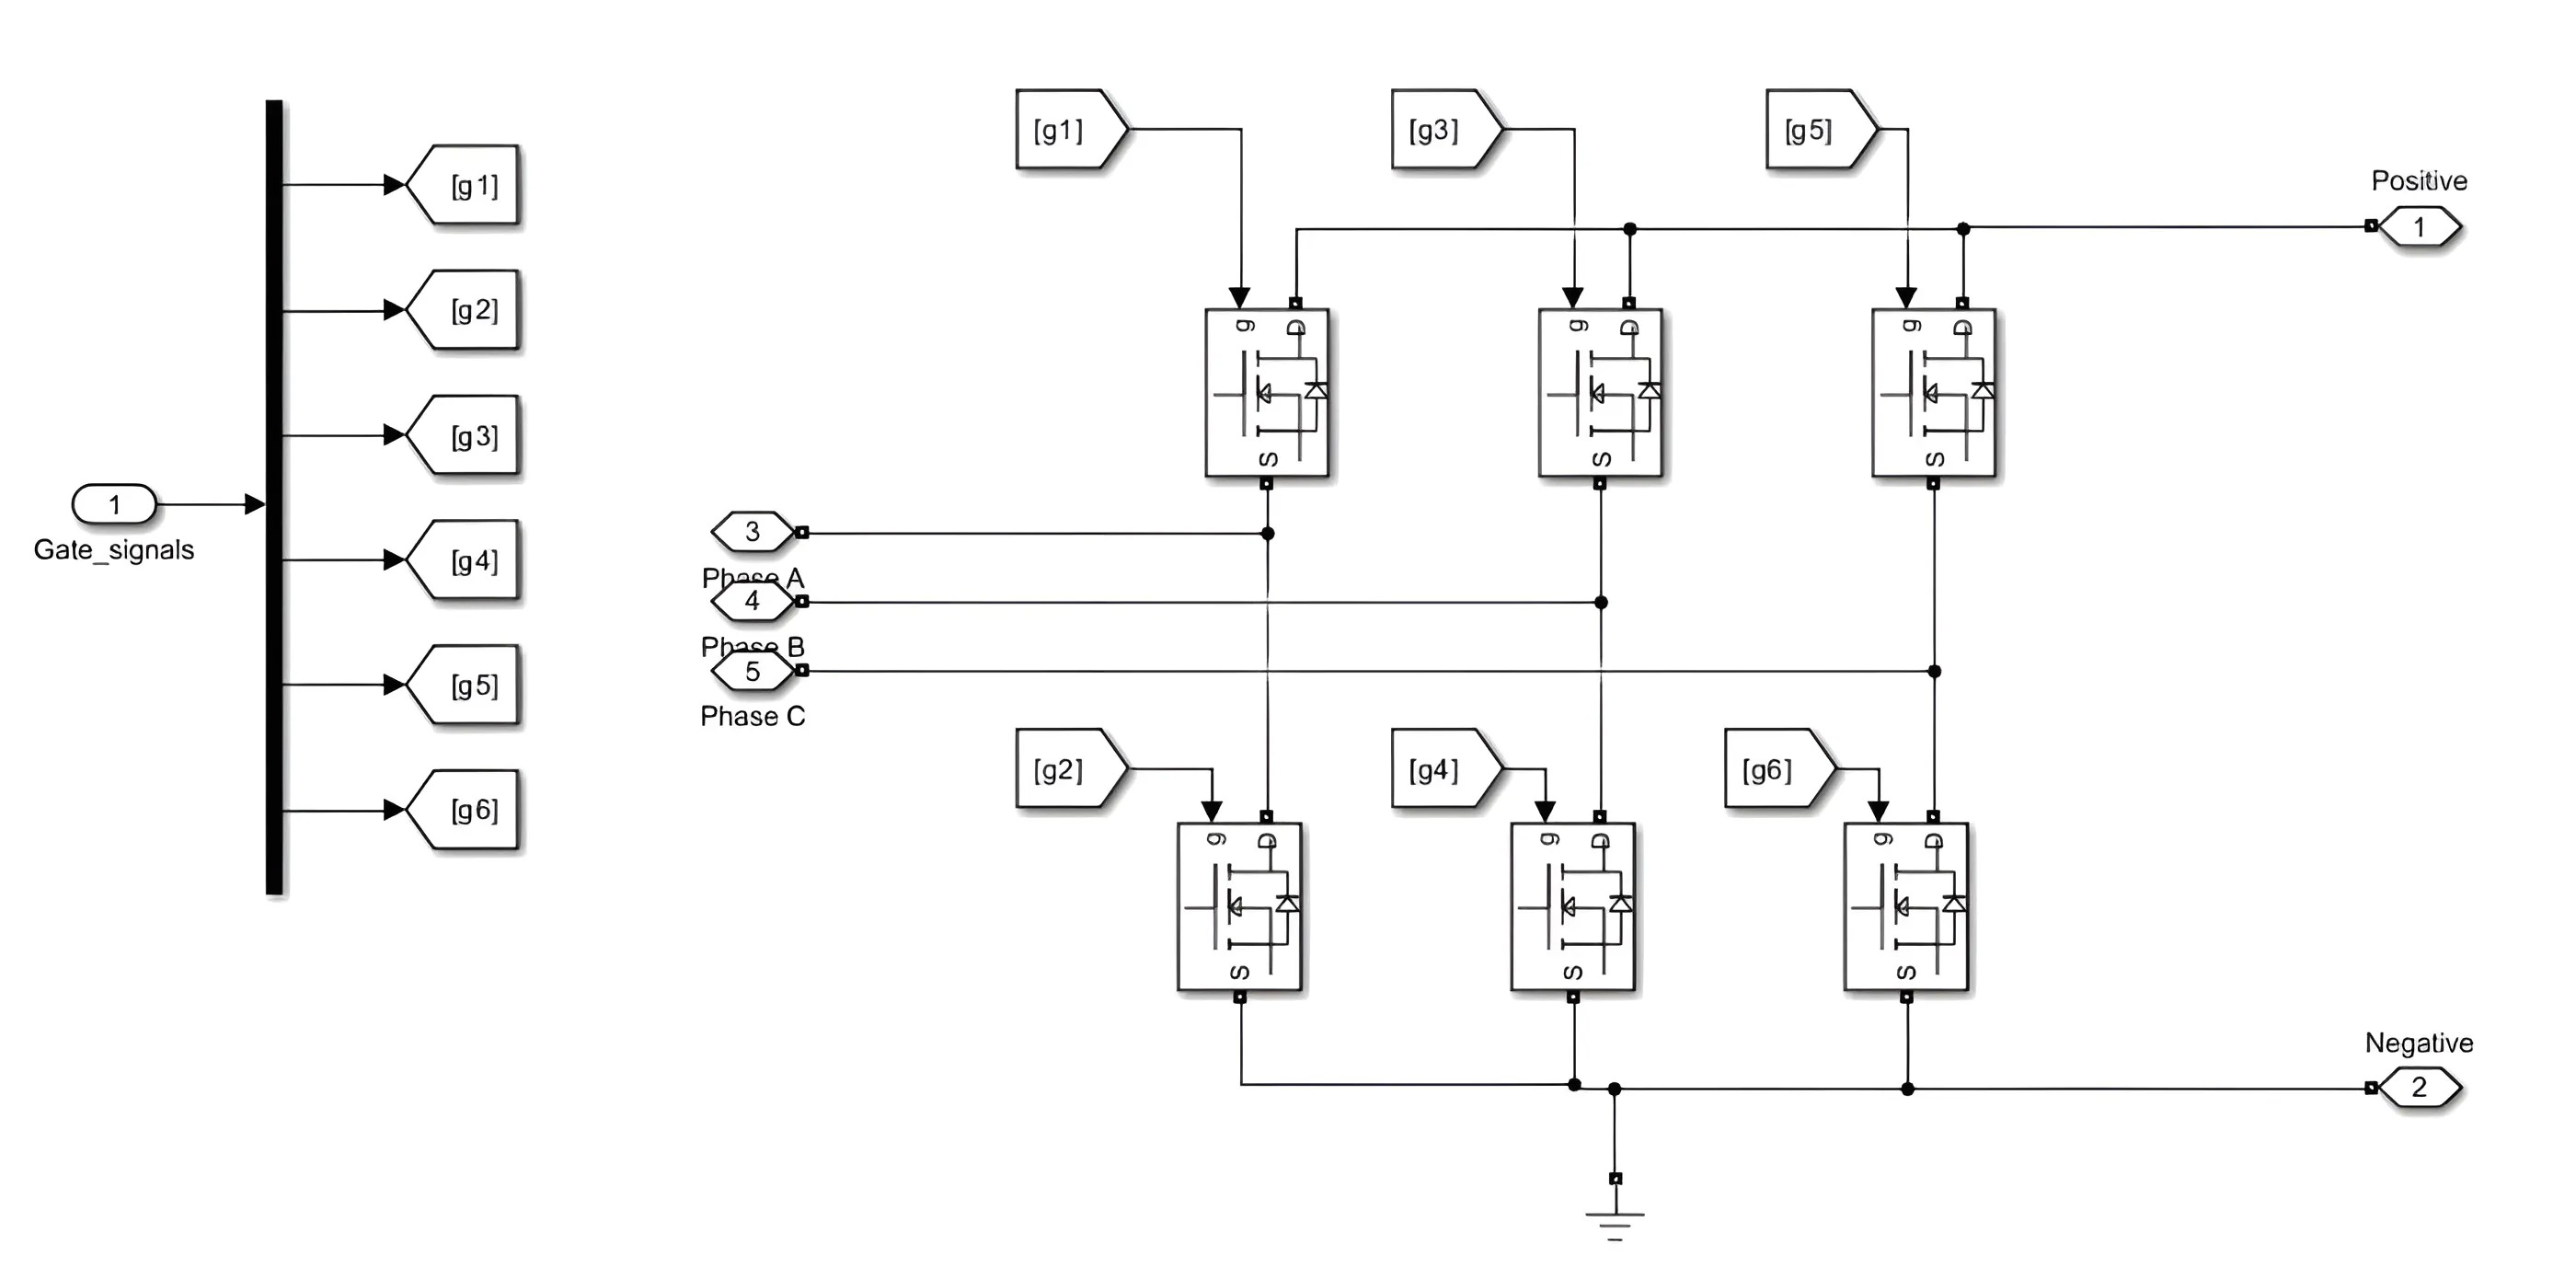
\includegraphics[width=1\textwidth]{inc/img/model4.png}
\caption{Трёхфазный инвертор}
\label{pic:mod4}
\end{figure}

\begin{figure}[!h]
\centering
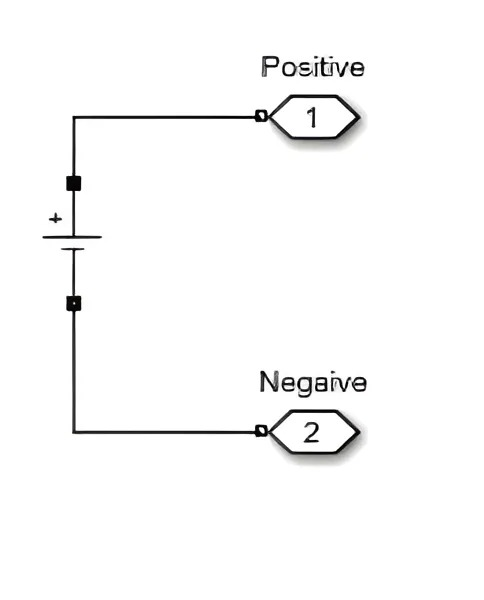
\includegraphics[width=0.3\textwidth]{inc/img/model3.png}
\caption{Источник постоянного тока}
\label{pic:mod3}
\end{figure}

Переключение ключей происходит по текущему электрическому положению ротора с использованием ШИМ, скважность которого регулируется в зависимости от модуля значения выхода значения, получаемого на выходе ПИ регулятора контура момента, выход которого ограничен диапазоном от $-1$ до $1$ (Рисунок \ref{pic:mod7}).

\begin{figure}[!h]
\centering
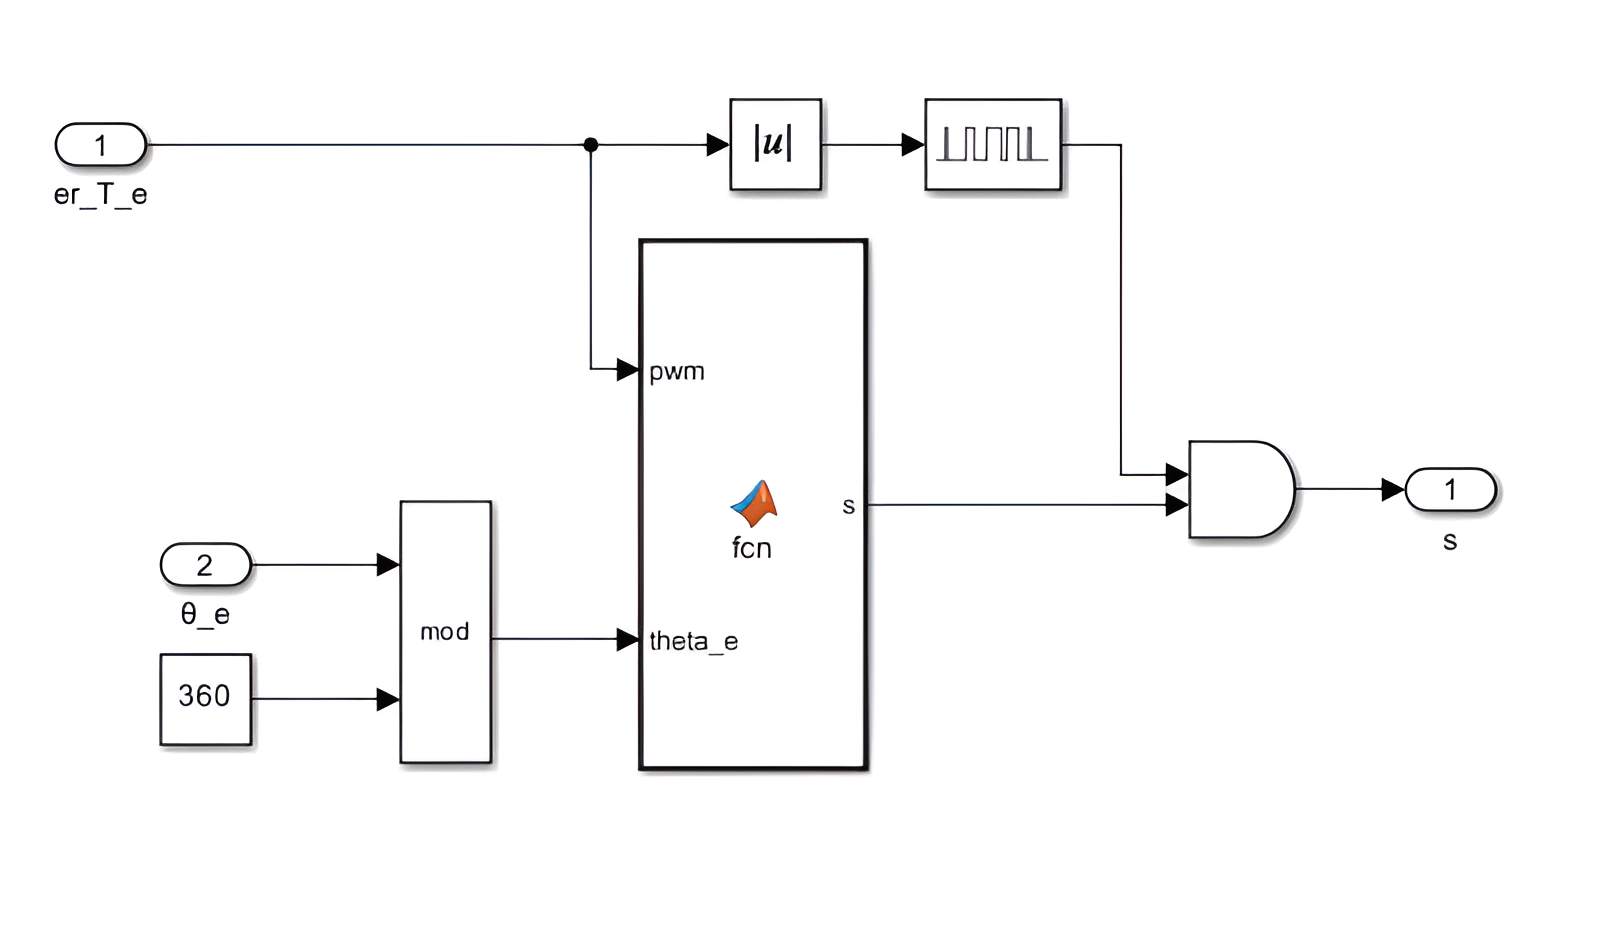
\includegraphics[width=0.7\textwidth]{inc/img/model7.png}
\caption{Система переключения ключей инвертора}
\label{pic:mod7}
\end{figure}

Возможные состояния в $\alpha-\beta$ системе с состояниями ключей приведены на Рисунке \ref{pic:vectors_dtc} и таблица коммутации в зависимости от электрического положения ротора и выхода ПИ регулятора момента приведены в Таблице \ref{table:com_dtc}.

\begin{figure}[!h]
\centering
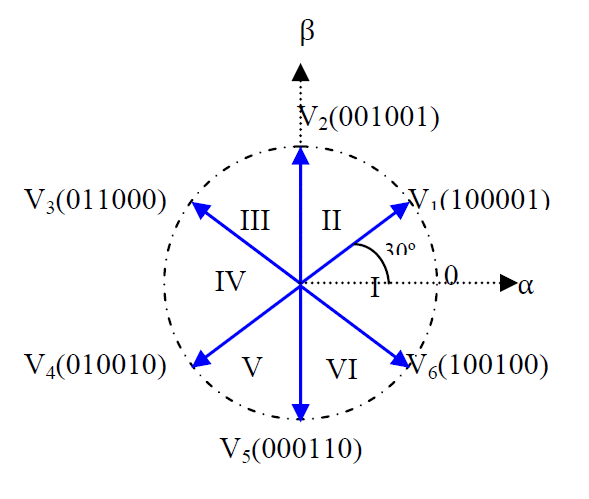
\includegraphics[width=0.7\textwidth]{inc/img/dtc_vectors.png}
\caption{Векторы переключения и состояния ключей \cite{art:dtc_smo}}
\label{pic:vectors_dtc}
\end{figure}

\begin{center}
\captionof{table}{схема коммутации от выхода регулятора\label{table:com_dtc}}
\begin{tabular}{|c|p{1.5cm}|p{1.5cm}|p{1.5cm}|p{1.5cm}|p{1.5cm}|p{1.5cm}|}
 \hline
 Выход ПИ регулятора & \multicolumn{6}{c|}{Электрическое положения ротора, $^\circ$} \\
 \hline
 [$0$---$1$] & $V_2$ & $V_3$ & $V_4$ & $V_5$ & $V_6$ & $V_1$ \\ 
 \hline
 [$-1$---$0$) & $V_5$ & $V_6$ & $V_1$ & $V_2$ & $V_3$ & $V_4$ \\
 \hline
\end{tabular}
\end{center}

\section{Результаты моделирования}
\label{sec:model_res}

Для моделирования использовались следующие параметры:
\begin{enumerate}
	\item Параметры двигателя (значения взяты от реального двигателя (\ref{sec:choose}), который будет использоваться в дальнейшем):
	\begin{align*}
		&R_s = 0,1\textrm{ Ом}\\
		&L_s = 0,0225\textrm{ Гн}\\
		&p = 4\\
		&k_e = 0,909\textrm{ B*мин/об}
	\end{align*}
	\item Параметры наблюдателя:
	\begin{align*}
		&g = 0,9\\
		&\eta = 7,8821e-4\\
		&f_{\textrm{среза}}=1200\textrm{ Гц}
	\end{align*}, где $f_{\textrm{среза}}$ --- частота среза для фильтра нижних частот на выходе оценки противо-ЭДС для уменьшения чаттеринга
	\item Параметры ПИ регулятора контура скорости:
	\begin{align*}
		&K_p = 2,39\\
		&K_i = 0,05
	\end{align*}
	\item Параметры ПИ регулятора контура момента:
	\begin{align*}
		&K_p = 0,01\\
		&K_i = 0,09
	\end{align*}\
	\item Частота дискретизации:
	\begin{align*}
		T = 1e-6\textrm{ с}
	\end{align*}
\end{enumerate}

Моделирования проводилось в трёх отрезках задачи скорости ($0-400$ рад/с, $400-600$ рад/с и $600-300$ рад/с) и каждый раз двигателю задавалось некоторая начальная скорость, ведь иначе при низких скоростях наблюдателю не получалось получить достаточно точную оценку противо-ЭДС для достижения желаемой скорости.

По техническому заданию нам не известны действительные значения сопротивления и индуктивности статора, известны лишь значения с погрешностью (в реальной работе двигателя эти параметры также могут варьироваться из-за нагрева двигателя в ходе работы, например, или других факторов), поэтому проводились моделирования также на граничных их значениях.

По результатам моделирования можно сказать, что вариация сопротивления практически не оказывает влияния на результаты работы наблюдателя и на переходные процессы в целом (Рисунки \ref{pic:R-}-\ref{pic:2R+}) в сравнении с эталонными параметрами (Рисунки \ref{pic:ideal} и \ref{pic:ideal2}), тогда как изменение индуктивности уменьшает скорость сходимости наблюдателя, что сказывается на времени переходного процесса и требует большего значения начальной скорости для достижения цели регулирования. Однако в пределах вариации параметров во всех экспериментах были выполнены требования, предъявляемые к алгоритму в техническом задании.

\begin{figure}[!h]
\centering
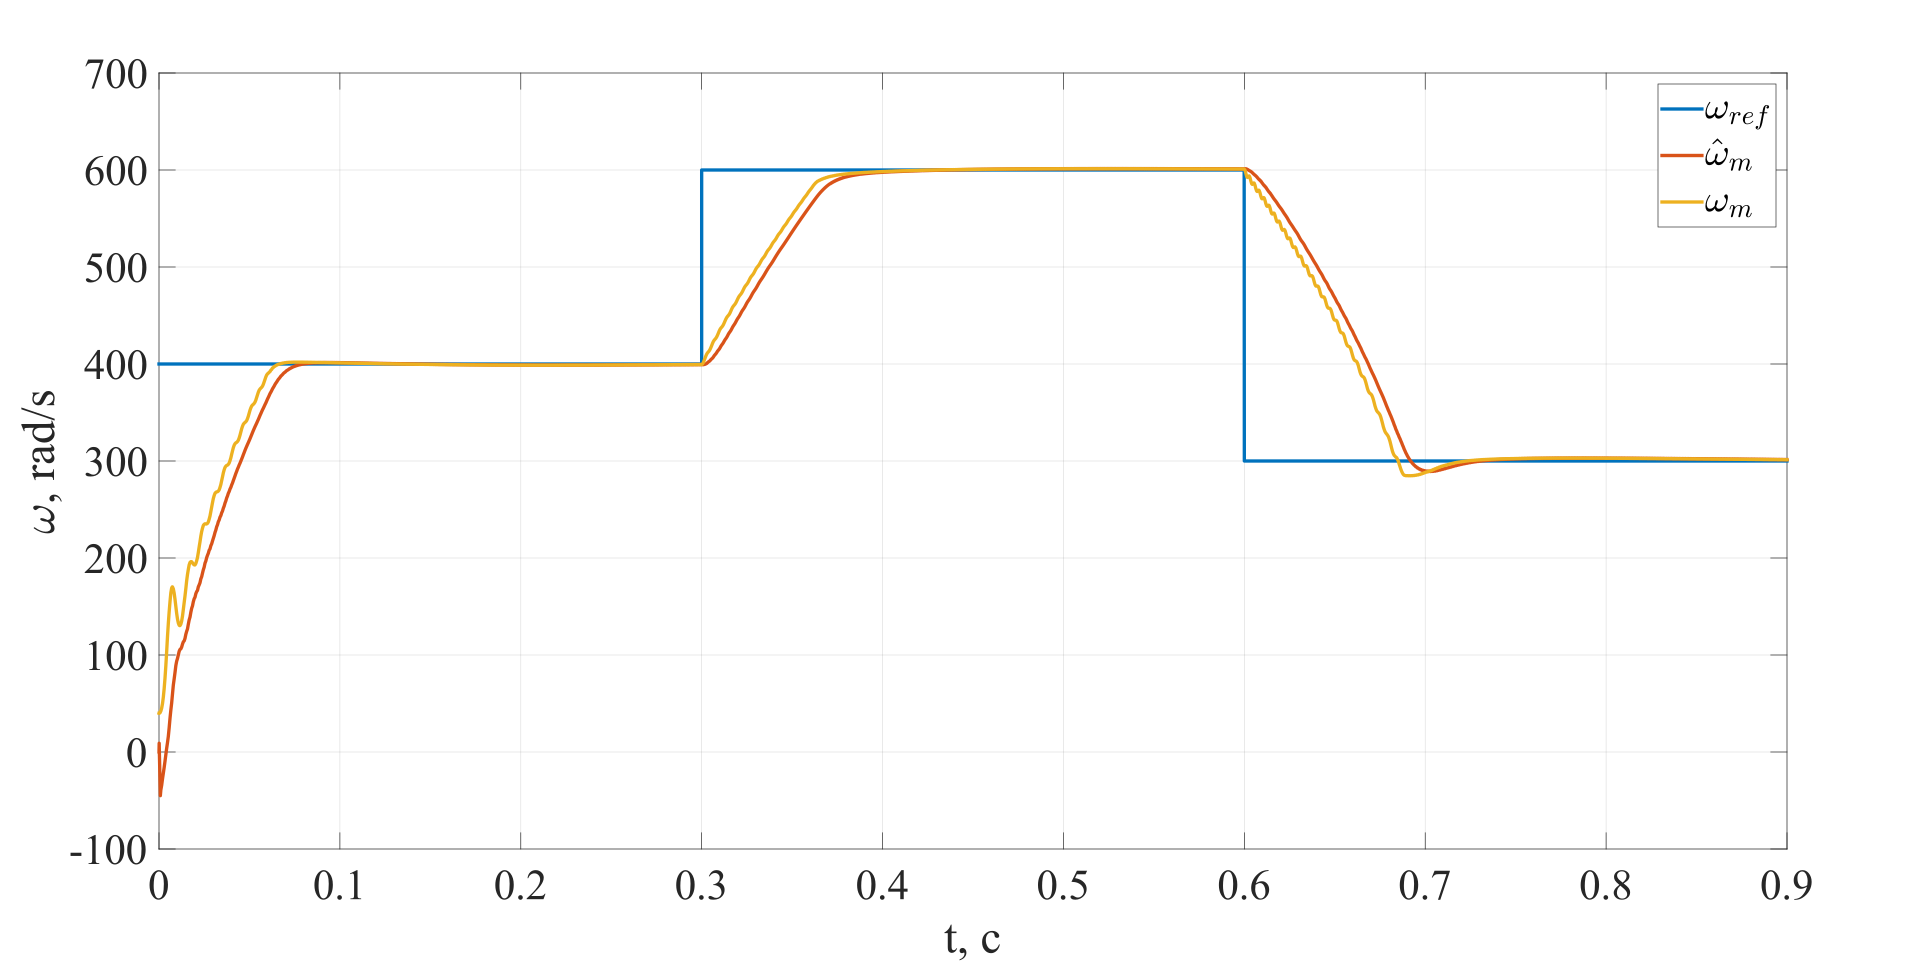
\includegraphics[width=\textwidth]{inc/svg/mod_resR}
\caption{Заданная, оцененная и действительная скорость ротора без вариации параметров}
\label{pic:ideal}
\end{figure}

\begin{figure}[!h]
\centering
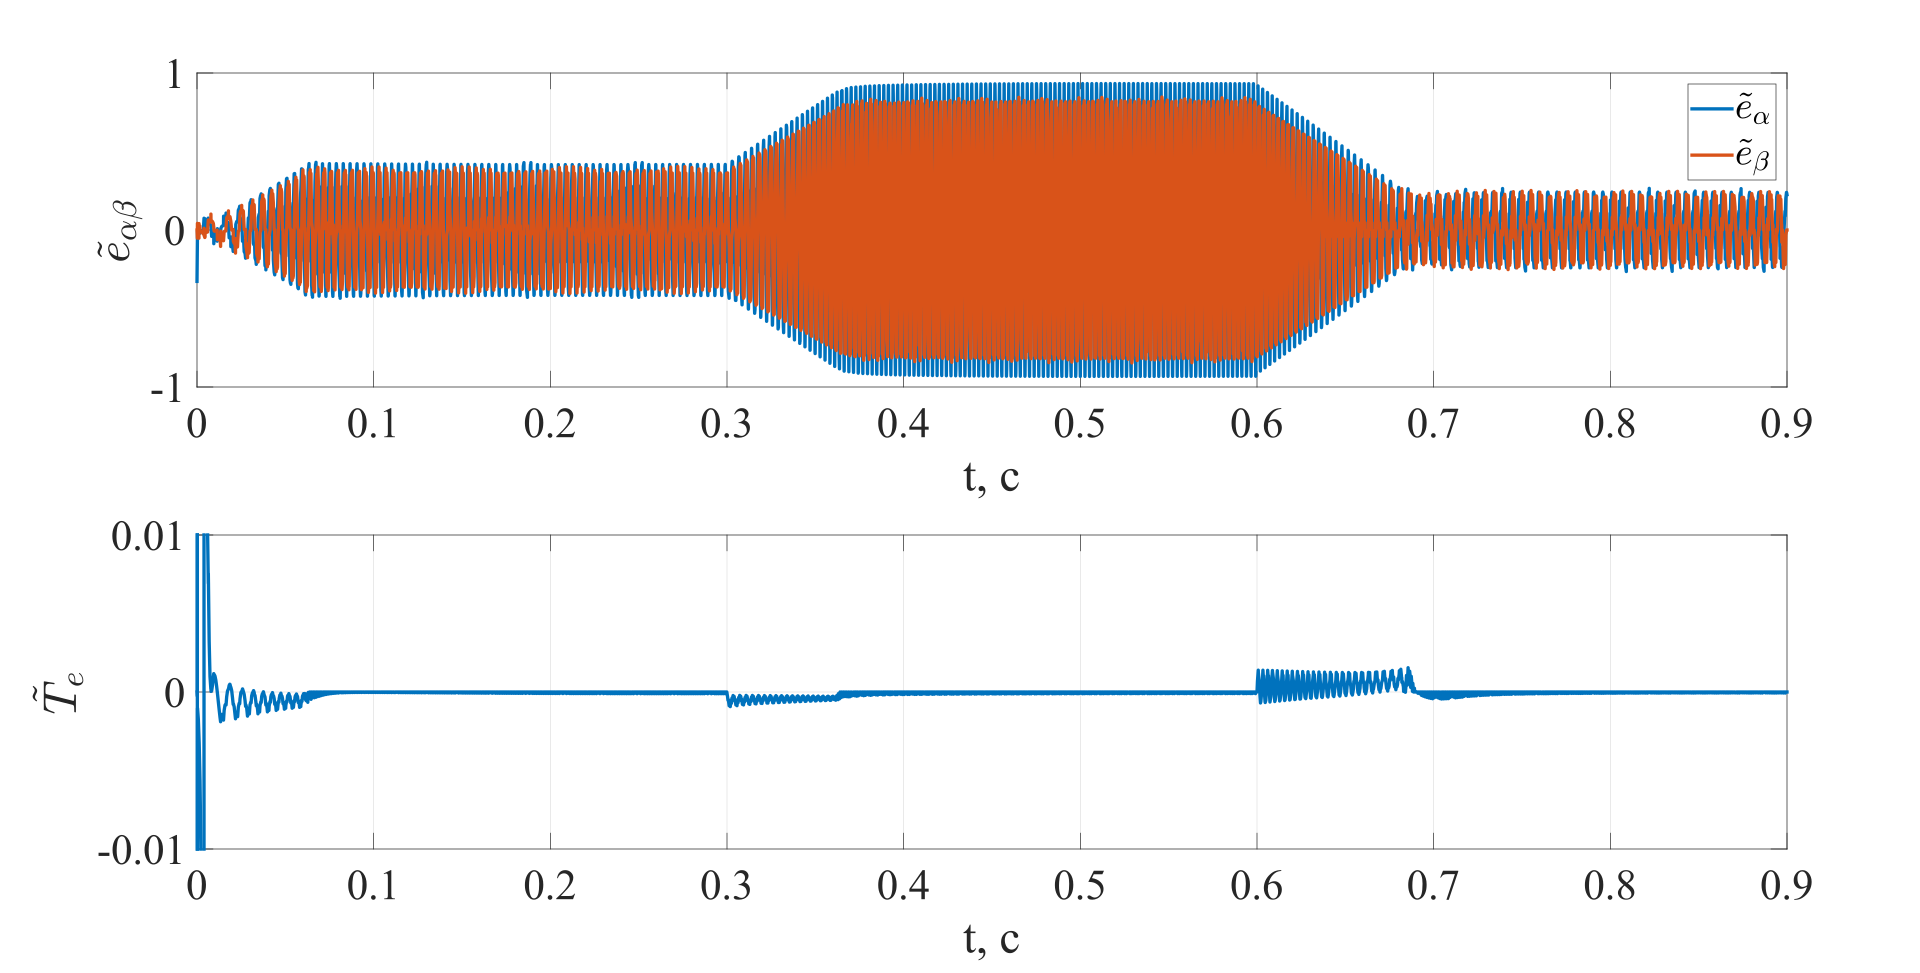
\includegraphics[width=\textwidth]{inc/svg/mod_res2R}
\caption{Вектор невязки по противо-ЭДС и электромагнитному моменту без вариации параметров}
\label{pic:ideal2}
\end{figure}

\begin{figure}[!h]
\centering
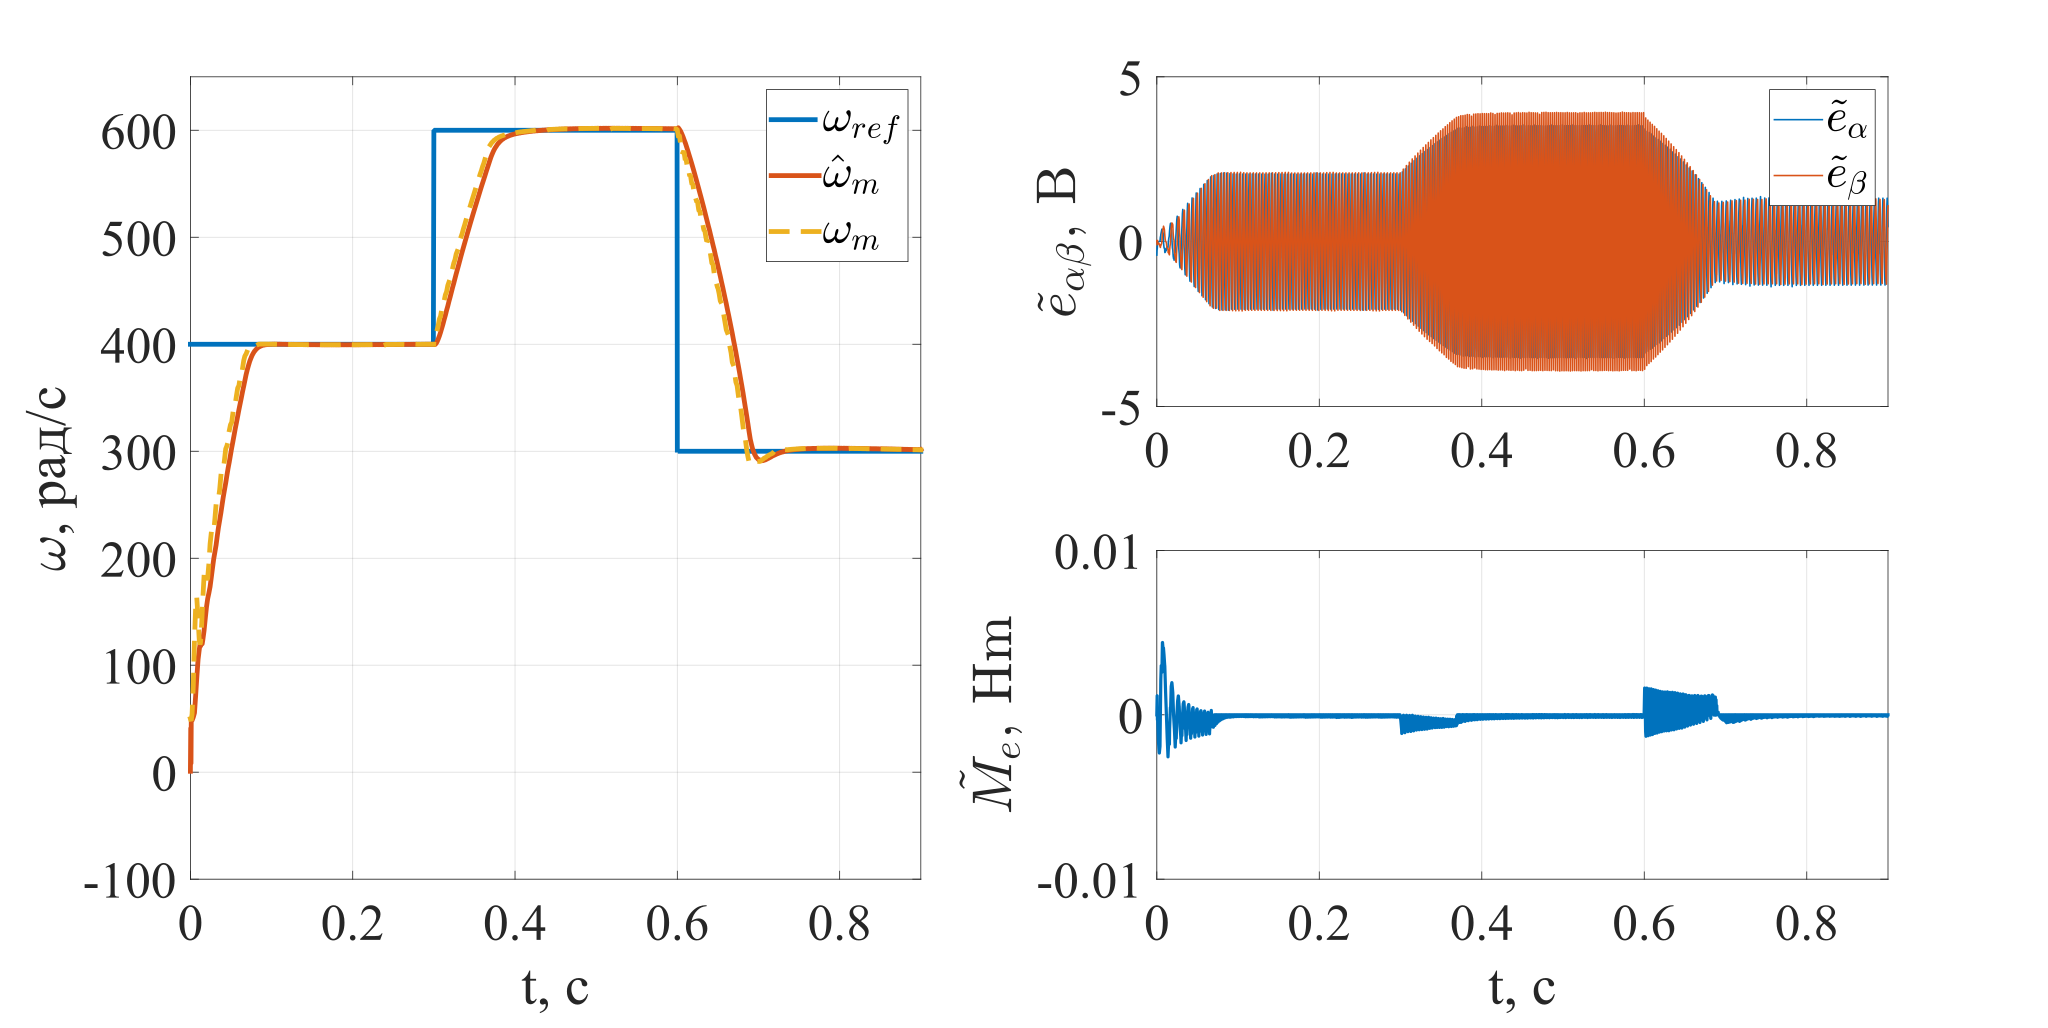
\includegraphics[width=\textwidth]{inc/svg/mod_resR-}
\caption{Заданная, оцененная и действительная скорость ротора при уменьшении $R$ на $100$ \%}
\label{pic:R-}
\end{figure}

\begin{figure}[!h]
\centering
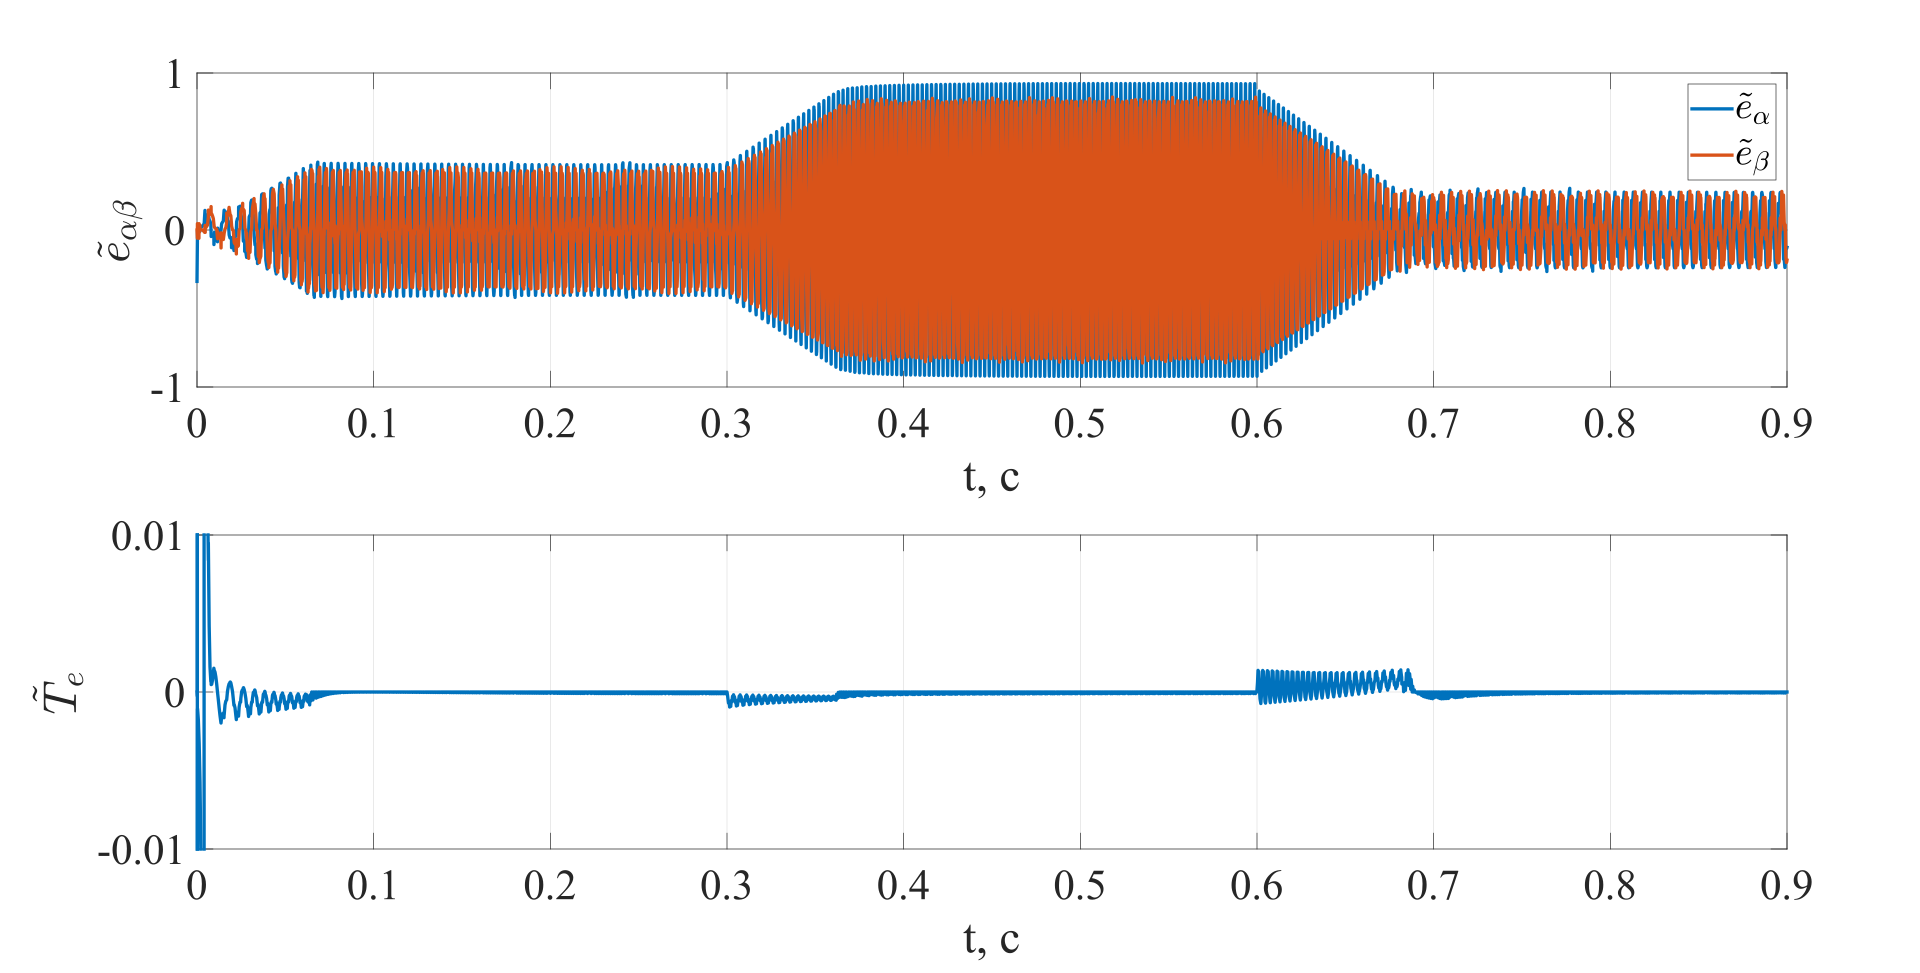
\includegraphics[width=\textwidth]{inc/svg/mod_res2R-}
\caption{Вектор невязки по противо-ЭДС и электромагнитному моменту при уменьшении $R$ на $100$ \%}
\label{pic:2R-}
\end{figure}

\begin{figure}[!h]
\centering
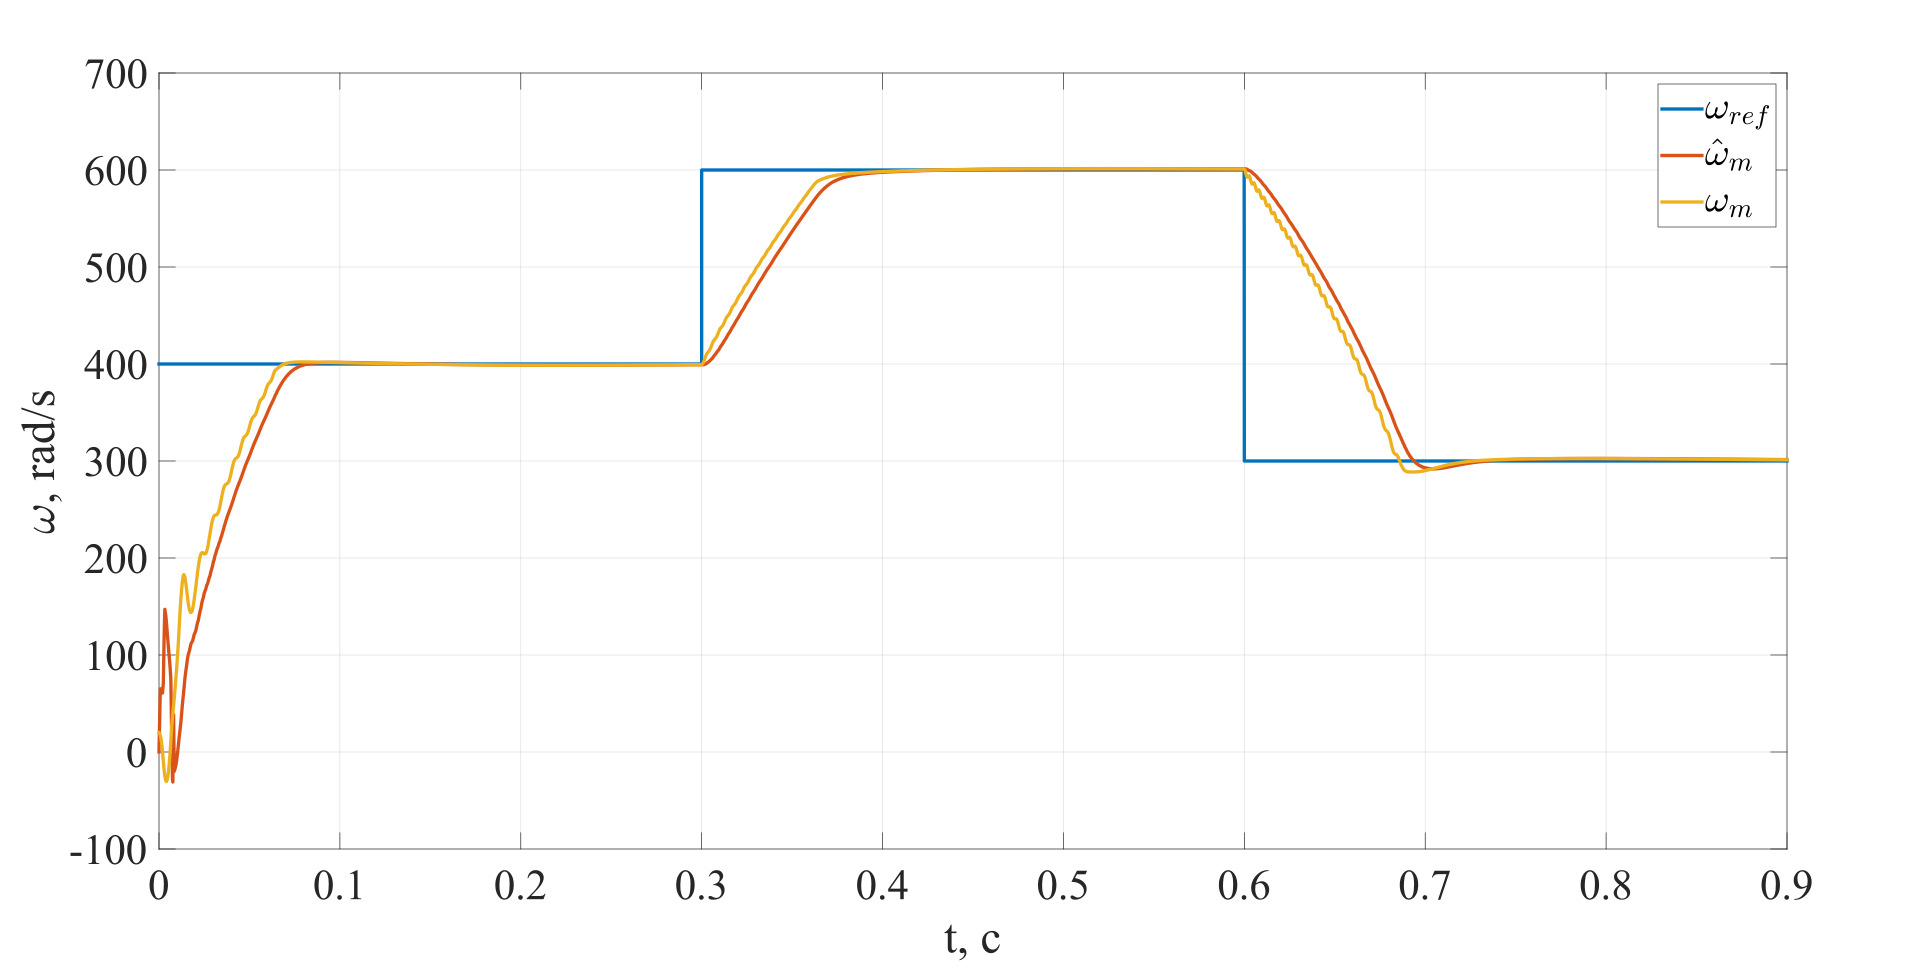
\includegraphics[width=\textwidth]{inc/svg/mod_resR+}
\caption{Заданная, оцененная и действительная скорость ротора при увеличении $R$ на $100$ \%}
\label{pic:R+}
\end{figure}

\begin{figure}[!h]
\centering
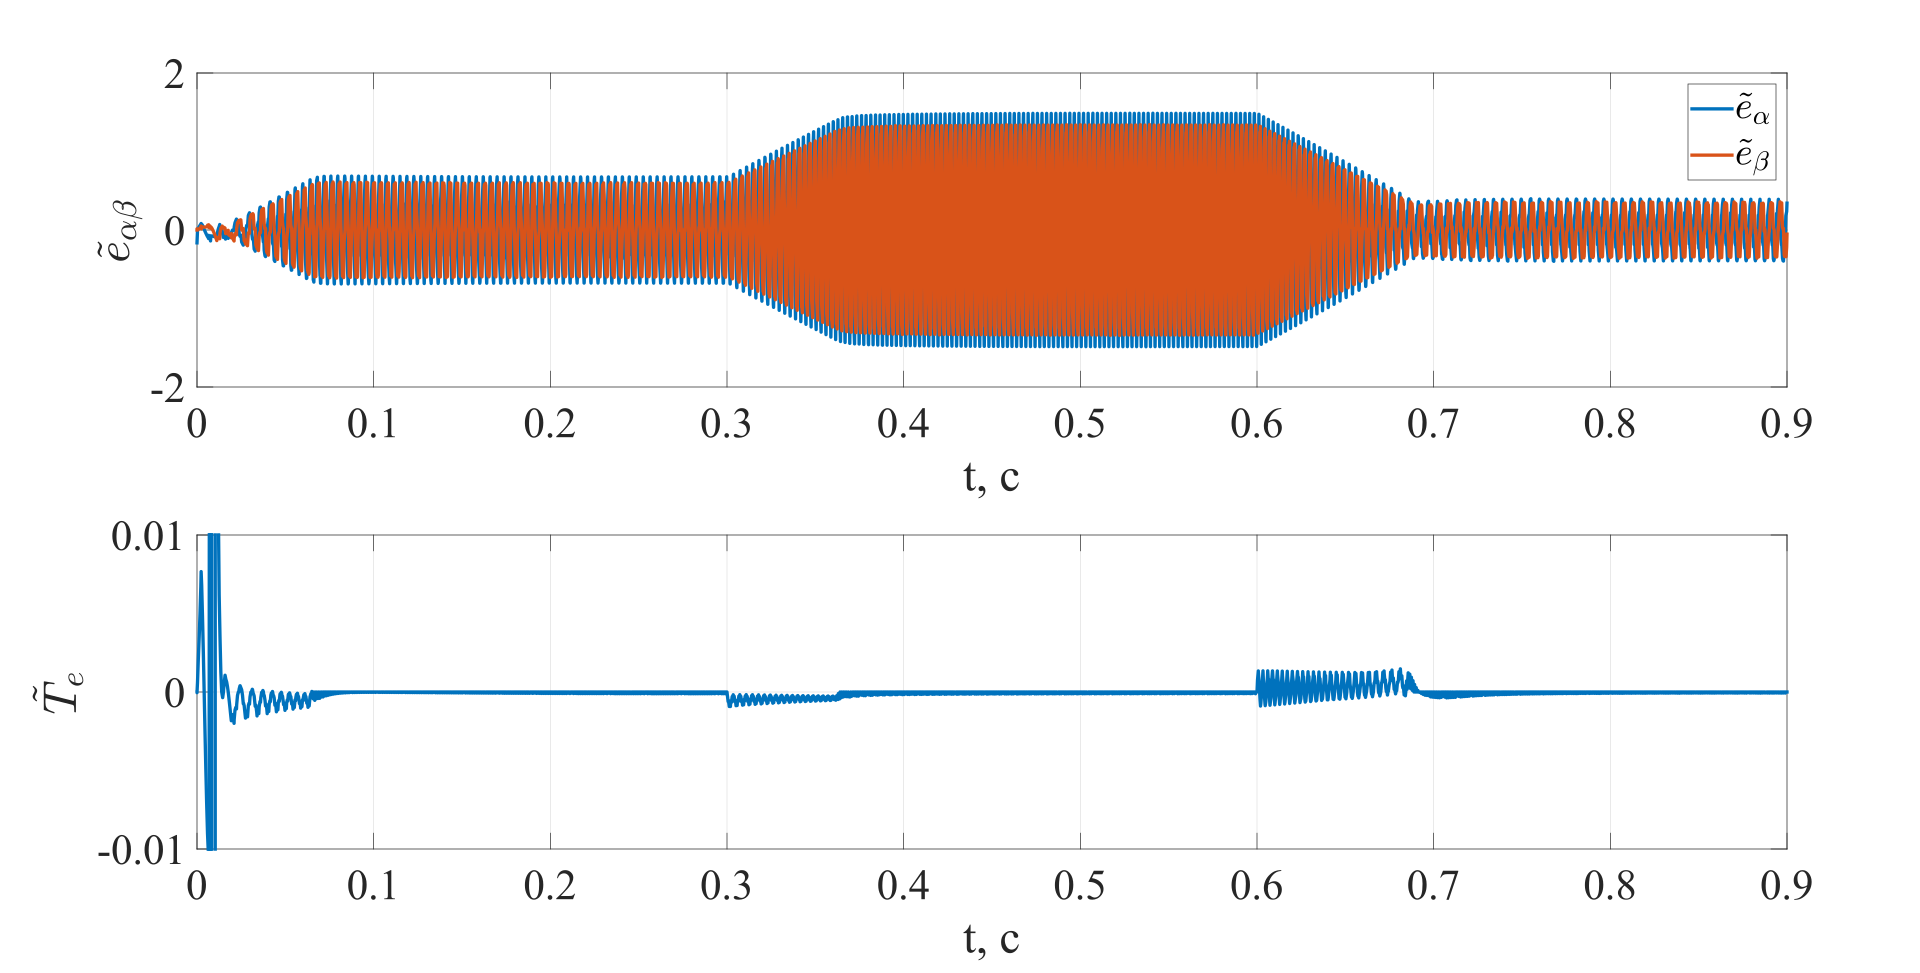
\includegraphics[width=\textwidth]{inc/svg/mod_res2R+}
\caption{Вектор невязки по противо-ЭДС и электромагнитному моменту при увеличении $R$ на $100$ \%}
\label{pic:2R+}
\end{figure}

\begin{figure}[!h]
\centering
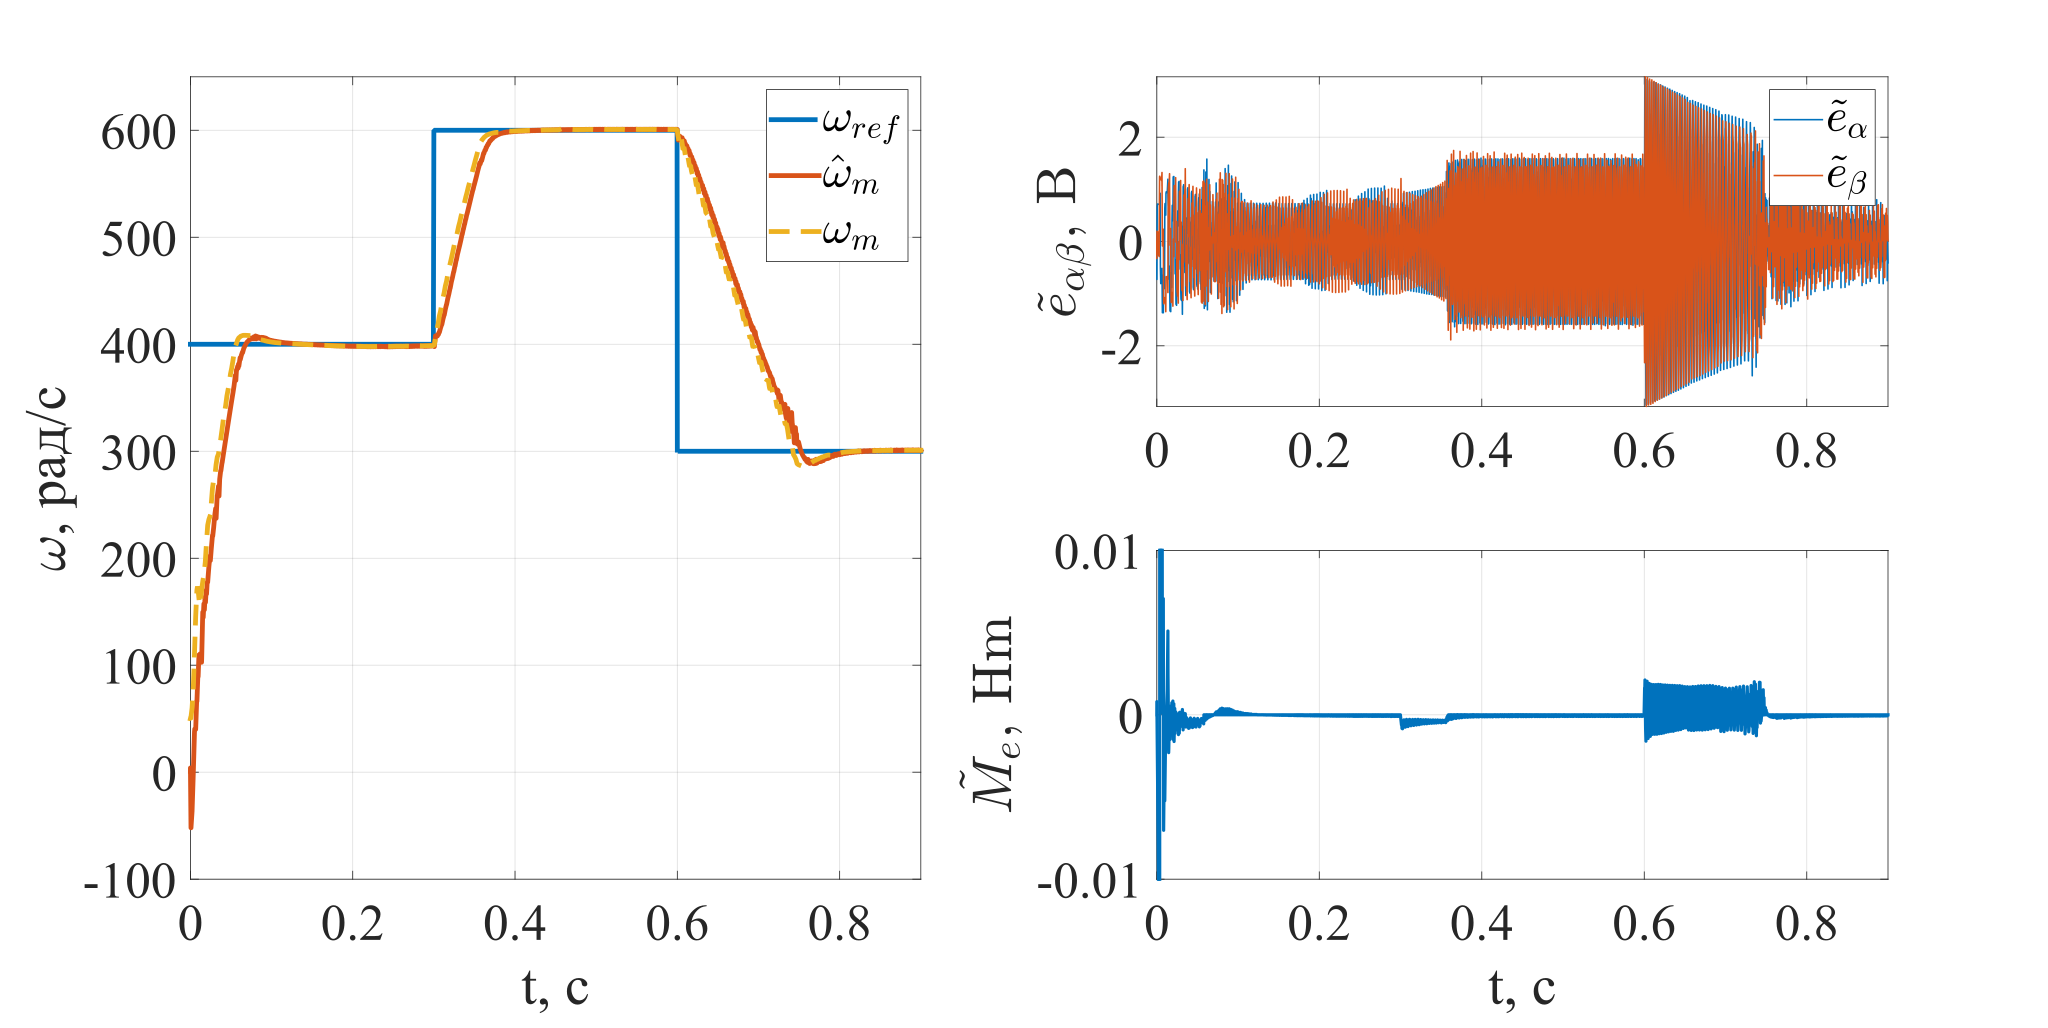
\includegraphics[width=\textwidth]{inc/svg/mod_resL-}
\caption{Заданная, оцененная и действительная скорость ротора при уменьшении $L$ на $10$ \%}
\label{pic:L-}
\end{figure}

\begin{figure}[!h]
\centering
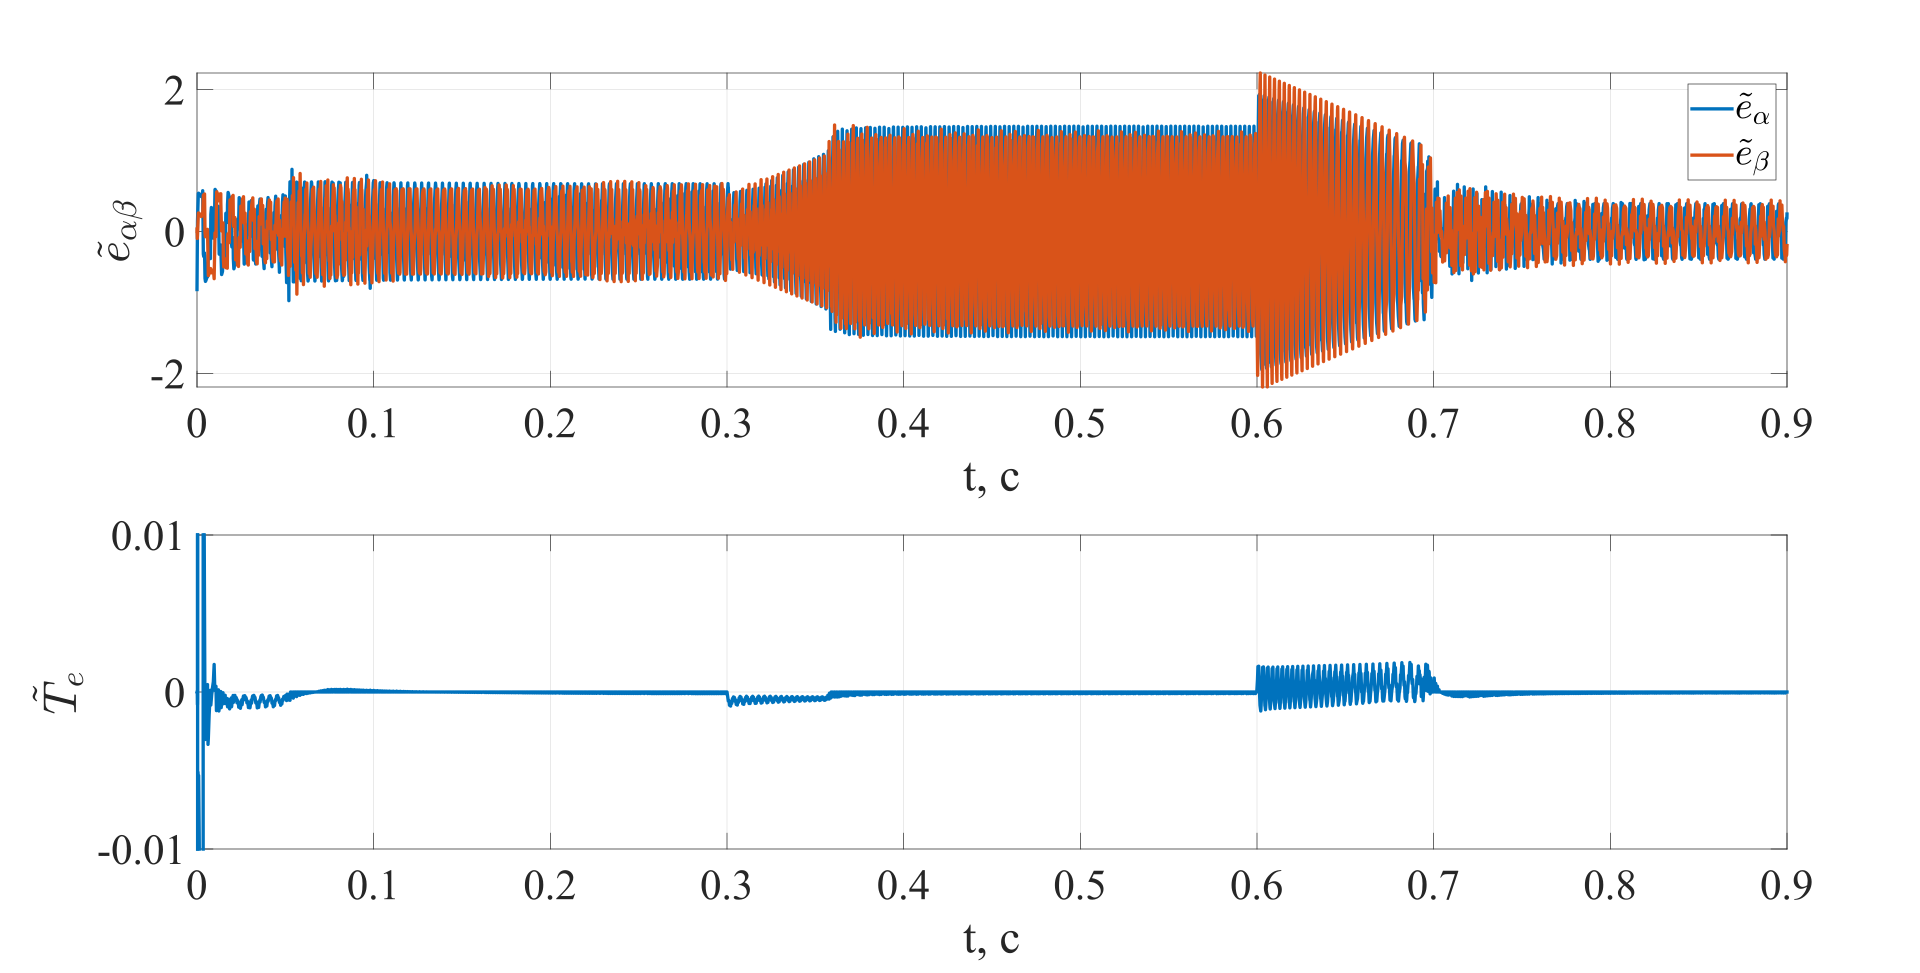
\includegraphics[width=\textwidth]{inc/svg/mod_res2L-}
\caption{Вектор невязки по противо-ЭДС и электромагнитному моменту при уменьшении $L$ на $10$ \%}
\label{pic:2L-}
\end{figure}

\begin{figure}[!h]
\centering
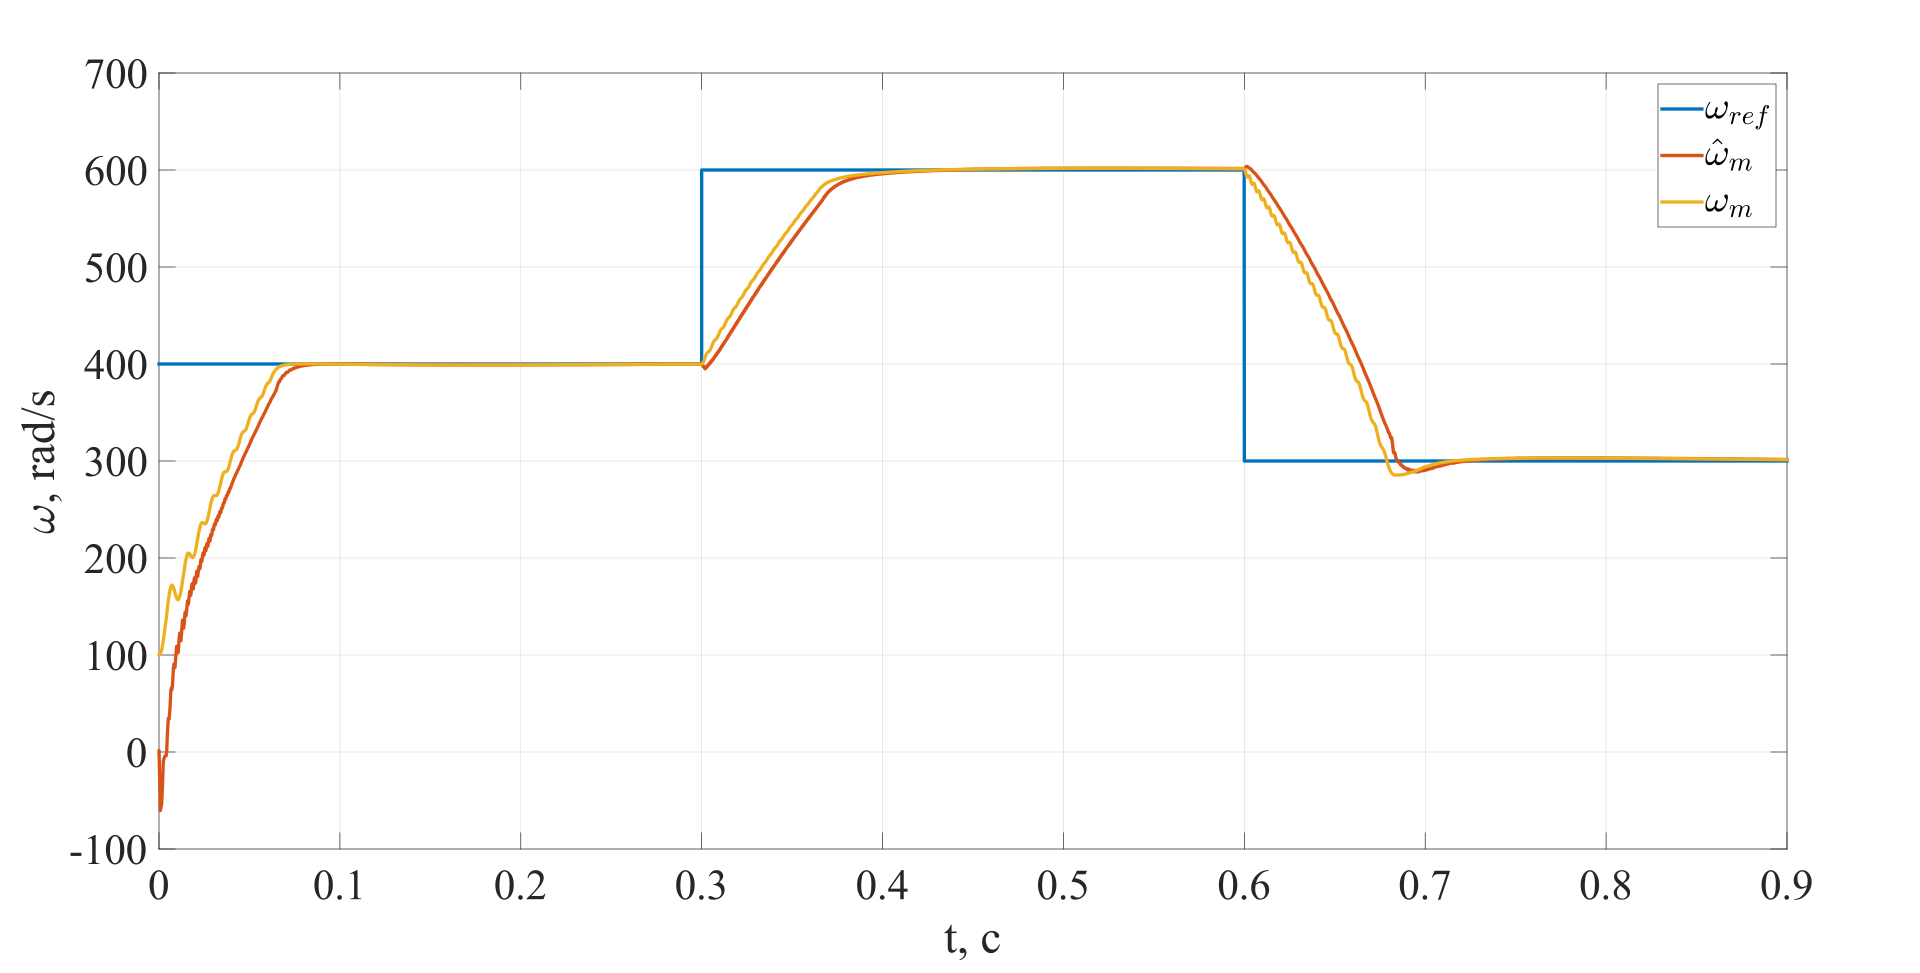
\includegraphics[width=\textwidth]{inc/svg/mod_resL+}
\caption{Заданная, оцененная и действительная скорость ротора при увеличении $L$ на $10$ \%}
\label{pic:L+}
\end{figure}

\begin{figure}[!h]
\centering
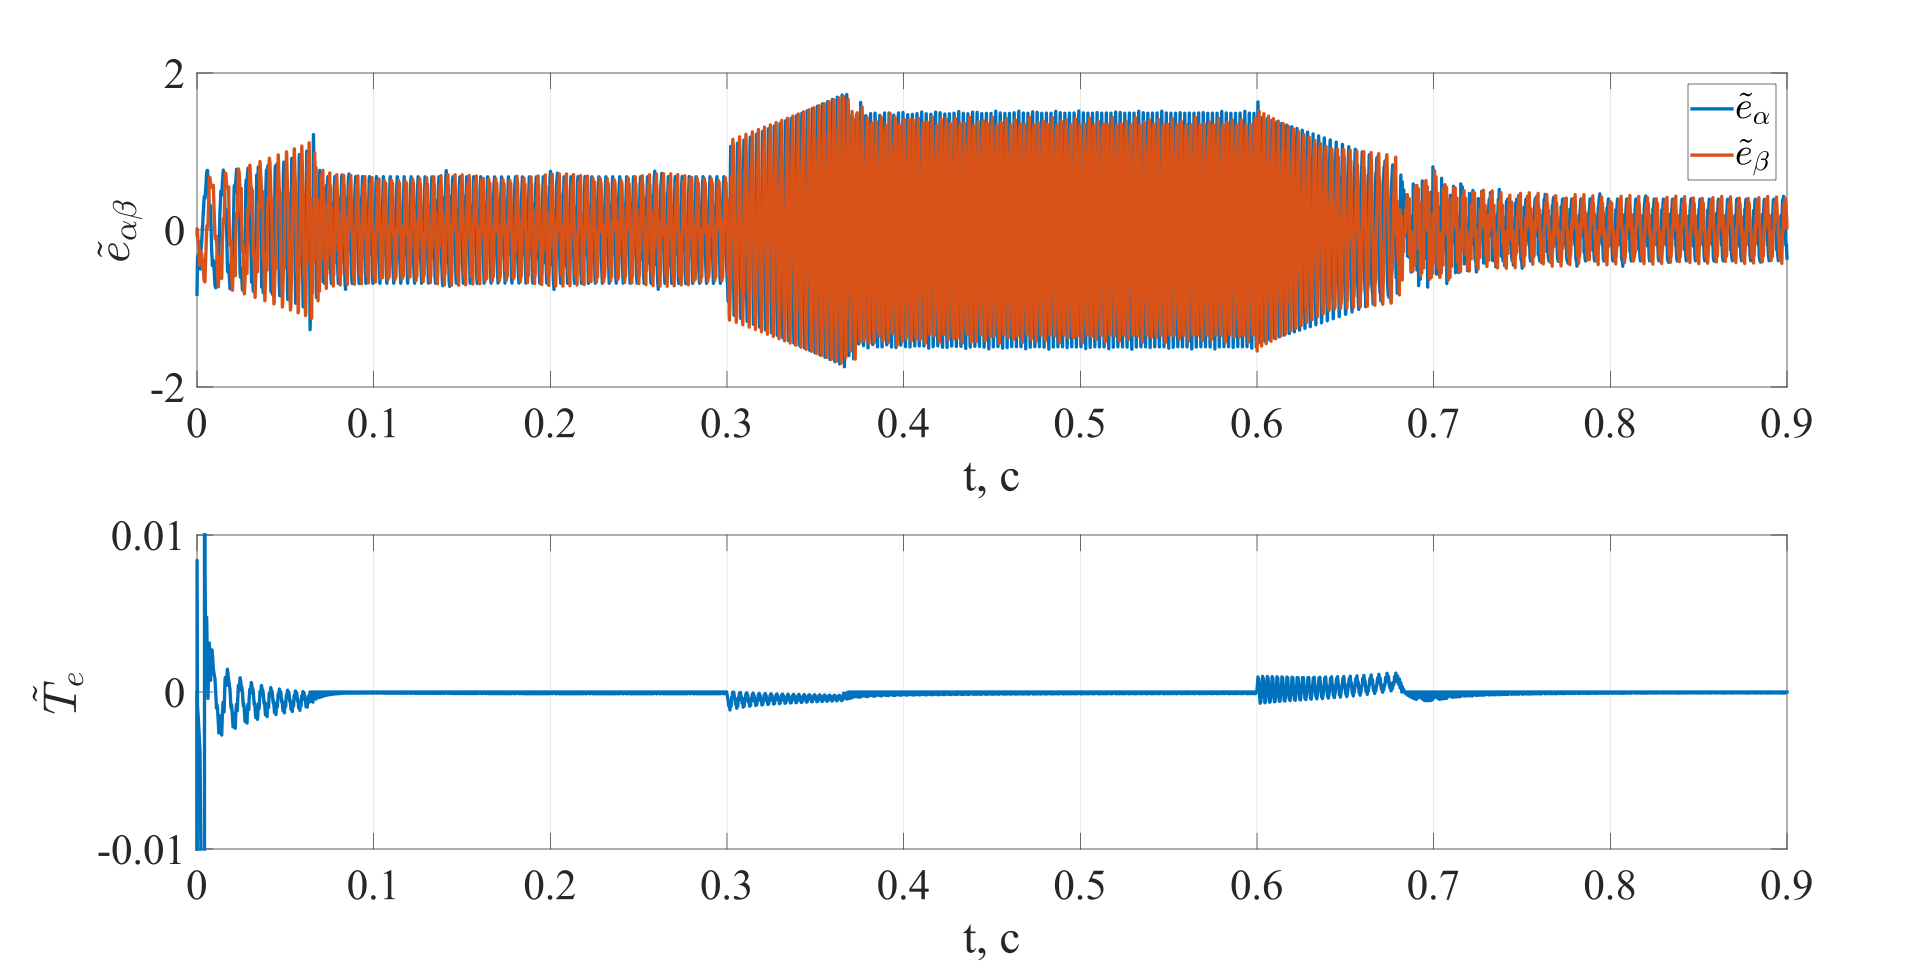
\includegraphics[width=\textwidth]{inc/svg/mod_res2L+}
\caption{Вектор невязки по противо-ЭДС и электромагнитному моменту при увеличении $L$ на $10$ \%}
\label{pic:2L+}
\end{figure}

\chapter{Разработка экспериментального стенда}
\label{cha:chap5}

\section{Выбор компонентов и устройств для реализации узлов системы}
\label{sec:choose}

В данном разделе будут определены элементы и устройства для реализации узлов, определённых в \ref{sec:nodes}.

В качестве мозга для реализации алгоритма управления был выбран микроконтроллер STM32F411RET (Рисунок \ref{pic:mc}), который содержит всю необходимую периферию  (поддерживает генерацию ШИМ, имеет аналого-цифровой преобразователь (АЦП), таймеры и имеет возможность передачи информации по последовательный протоколу связи).

\begin{figure}[!h]
\centering
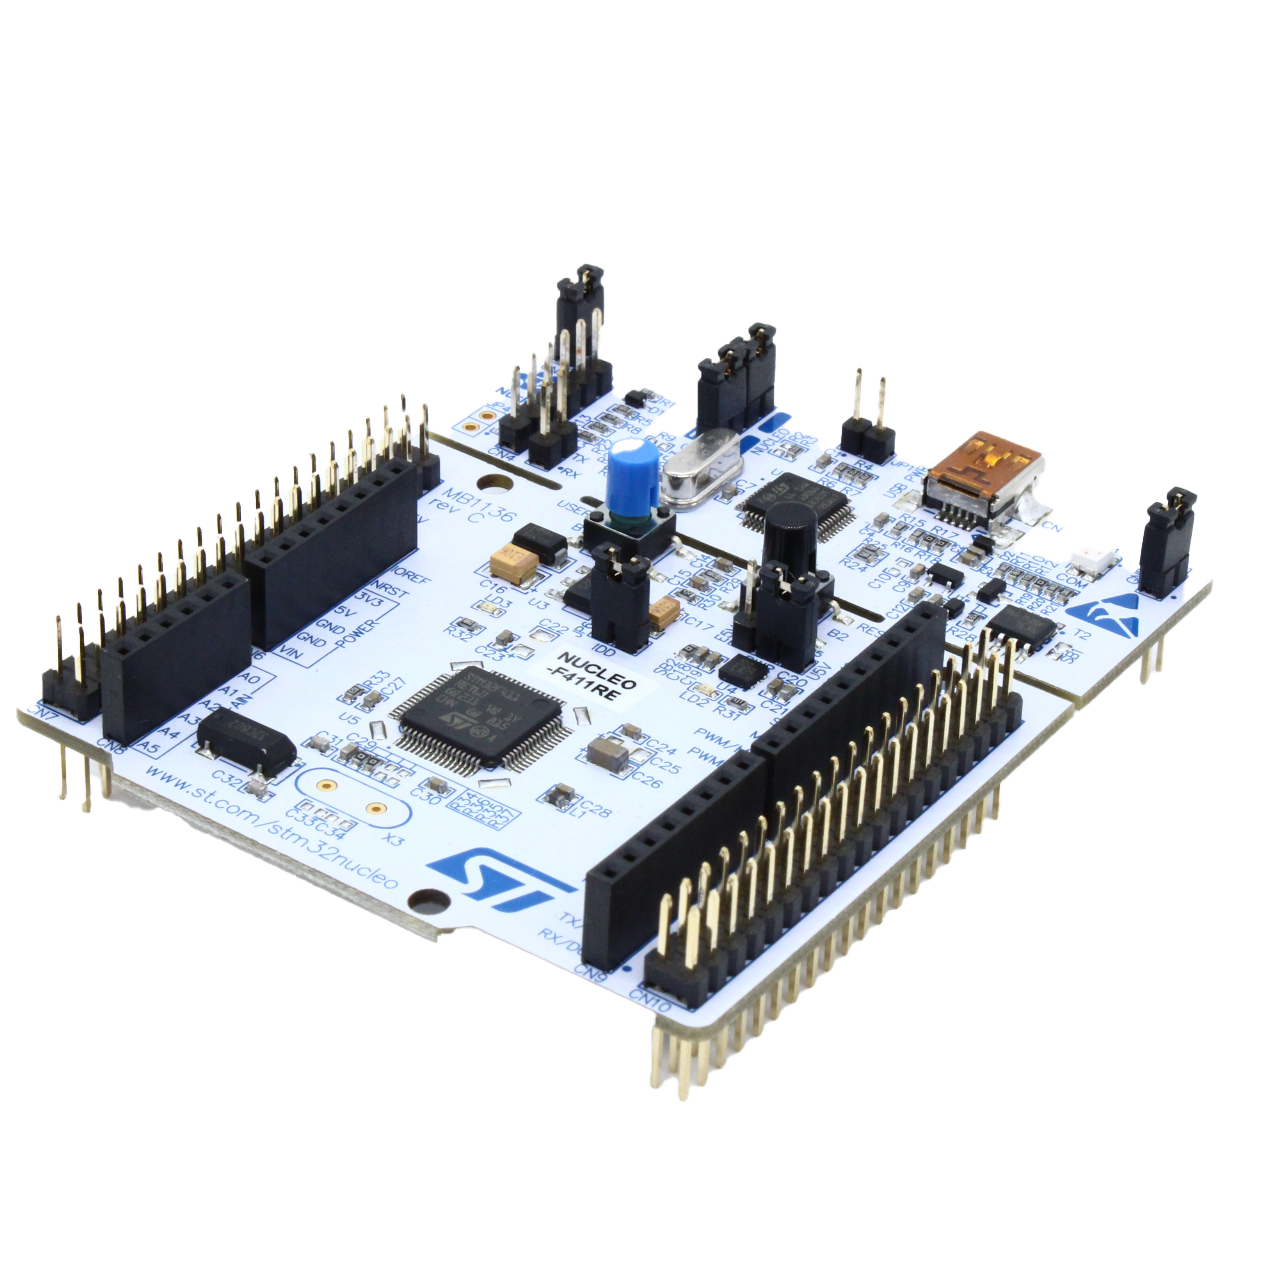
\includegraphics[width=0.7\textwidth]{inc/img/mc.png}
\caption{Микроконтроллер STM32F411RET на базе Nucleo64}
\label{pic:mc}
\end{figure}

Инвертор, датчики для определения напряжения и тока фаз реализованы на отдельной печатной плате, рассмотренной в \ref{sec:driver}. 

За объект управления взят двигатель Racerstar BR2208 1100KV (Рисунок \ref{pic:motor}), параметры которого были перечислены при моделировании в \ref{sec:model_res}.

\begin{figure}[!h]
\centering

\includegraphics[width=0.5\textwidth]{inc/img/motor.png}
\caption{БДПТ Racestar BR2208 1100KV}
\label{pic:motor}
\end{figure}

Для питания двигателя был выбран блок питания на 12 В/5 А (Рисунок \ref{pic:power}), которого будет достаточно для питания двигателя в условиях работы без нагрузки или в условиях малых нагрузок и который обеспечит сохранность всей электрической схемы в случае короткого замыкания.

\begin{figure}[!h]
\centering
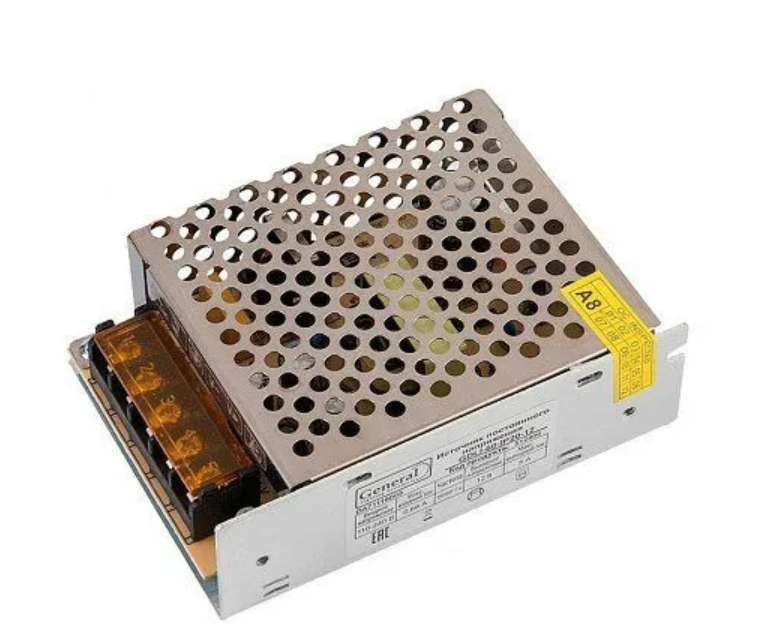
\includegraphics[width=0.7\textwidth]{inc/img/power.png}
\caption{Блок питания двигателя}
\label{pic:power}
\end{figure}
\clearpage
\section{Реализация драйвера двигателя}
\label{sec:driver}

Для реализации силовой части был спроектирован собственный драйвер БДПТ в среде проектирования Altium Designer.

\subsection{Инвертор}

Для 3-фазного инвертора были использованы полумостовые драйверы IR2104STRPBF для каждой фазы, которые служат для преобразования напряжений микроконтроллера в напряжения, достаточные для открытия ключей, в качестве которых выступают mosfet транзисторы IRLR2705PBF. Также драйверы выбранные драйверы транзисторов исключают возможность одновременного открытия верхнего и нижнего ключей, исключая возникновение короткого замыкания в этом случае.

Они имеют два входа для регулирования ($IN$ и $\overline{SD}$) и два выхода к транзисторам ($HO$ и $LO$). Зависимость сигналов выхода от значений входа изображена на Рисунке \ref{pic:driver_sw}. В нашем случае нижний вход будет служить для подачи на него ШИМ сигнала, а с помощью верхнего будет регулироваться, какой выход и, соответственно, какой транзистор открыть (при $IN=1$ открывается верхний ключ, при $IN=0$ открывается нижний ключ).

\begin{figure}[!h]
\centering
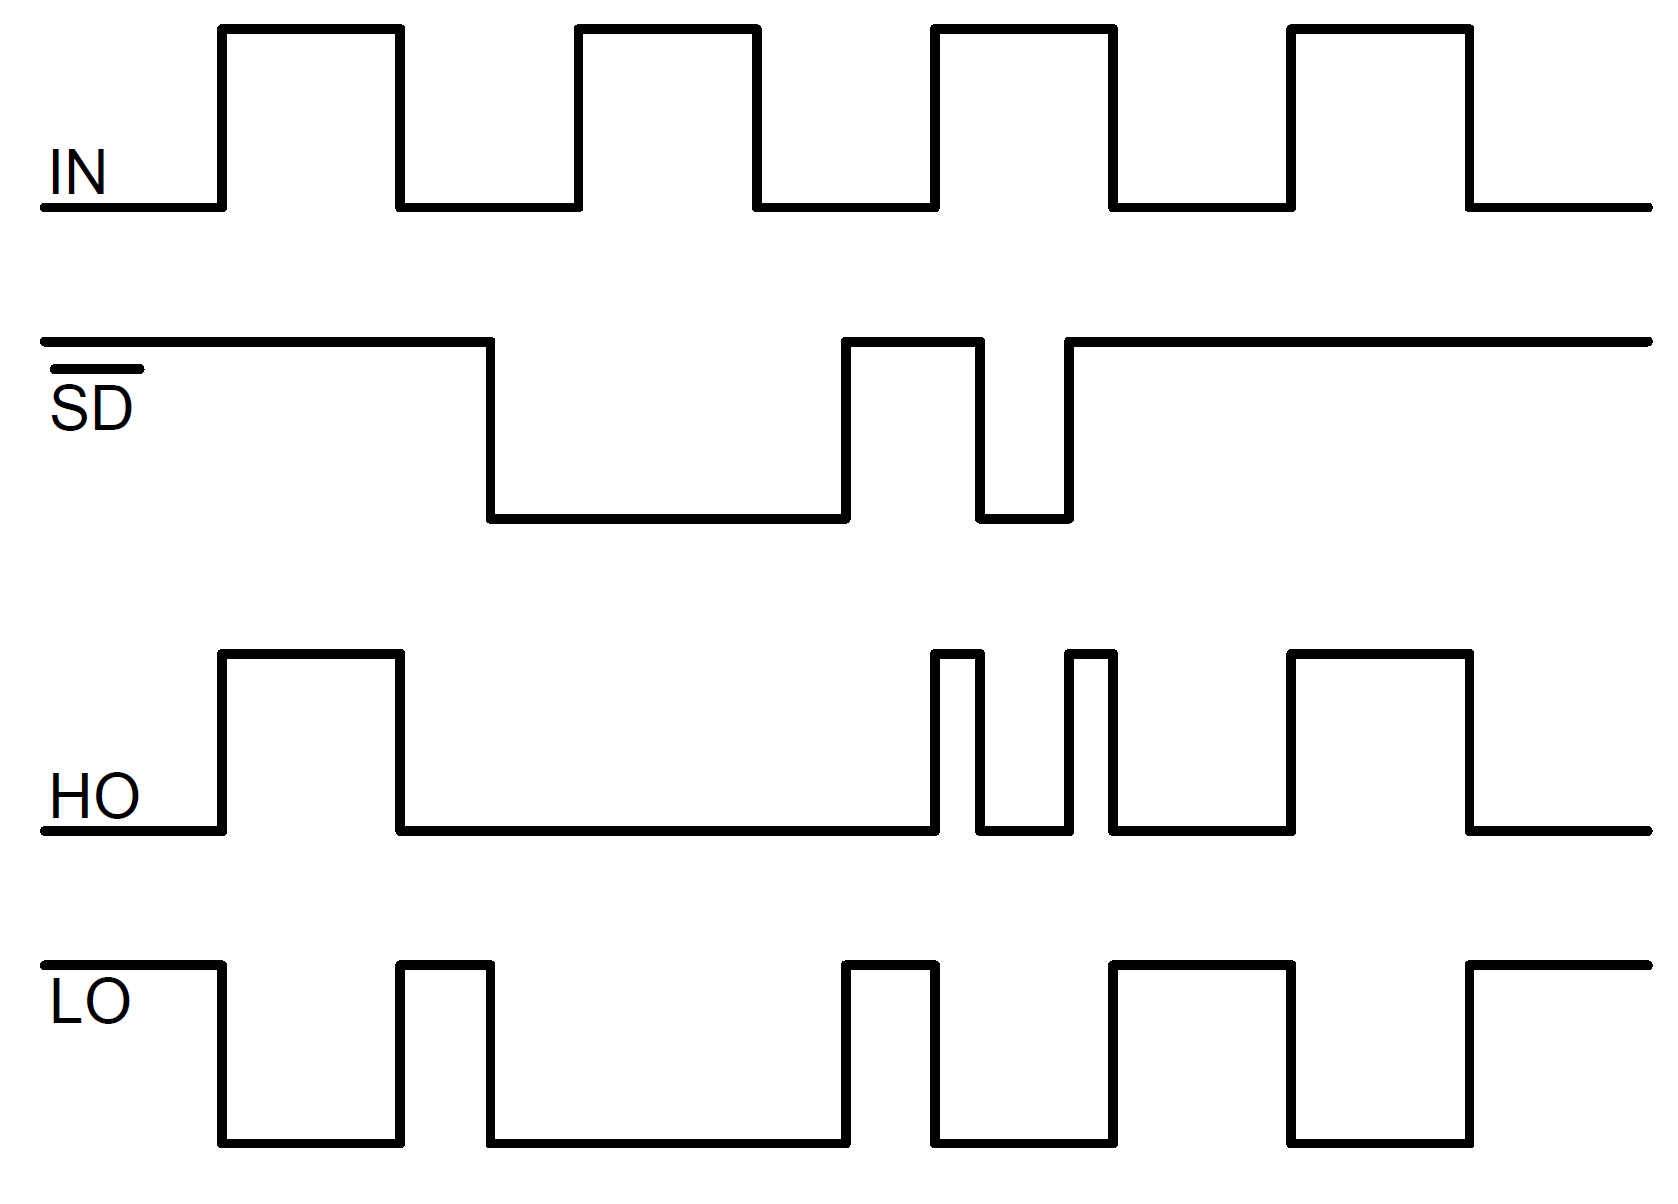
\includegraphics[width=0.7\textwidth]{inc/img/driver_sw.png}
\caption{Зависимость значений входов/выходов для IR2104STRPBF}
\label{pic:driver_sw}
\end{figure}

Также параллельно фазам двигателя установлены диоды, которые препятствуют протеканию обратного тока катушек, которыми являются фазы двигателя, во время смены состояния ключей.

Общая схема силовой части изображена на Рисунке \ref{pic:dr_power}.

\begin{figure}[!h]
\centering
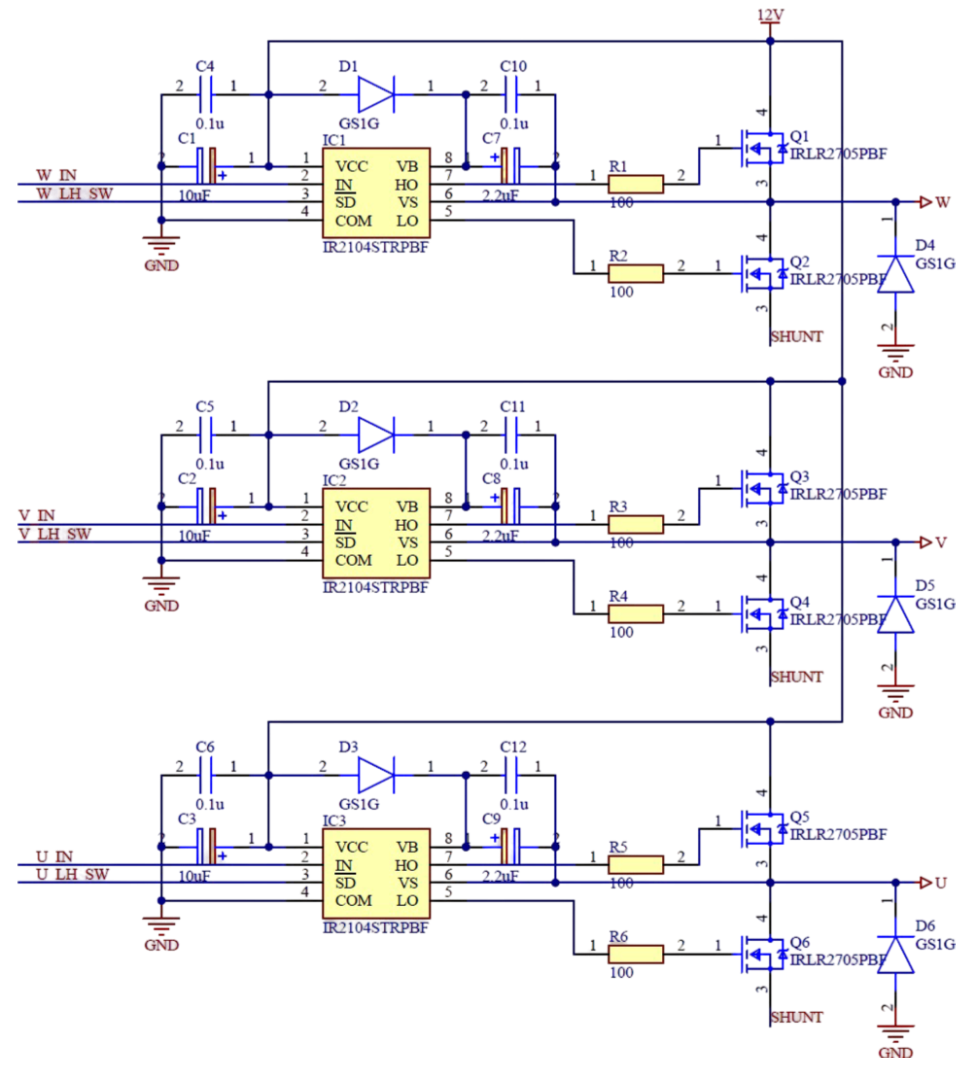
\includegraphics[width=\textwidth]{inc/img/dr_power.png}
\caption{Схема силовой части ($W$, $V$, $U$ --- фазы двигателя, $SHUNT$ --- сигнал, уходящий к датчику тока, $12V$ --- питание $12$ В, $WVU_{IN}$, $WVU_{LH_SW}$ --- входы для управления ключами драйвера)}
\label{pic:dr_power}
\end{figure}
\clearpage
\subsection{Измерительная часть}

Для измерения тока используется датчик тока на основе ACS712ELCTR-05B-T, позволяющий преобразовать ток, текущий через него в напряжение в диапазоне от $0$ до $5$ В. Схема измерения тока изображена на Рисунке \ref{pic:cur_sens}.

\begin{figure}[!h]
\centering
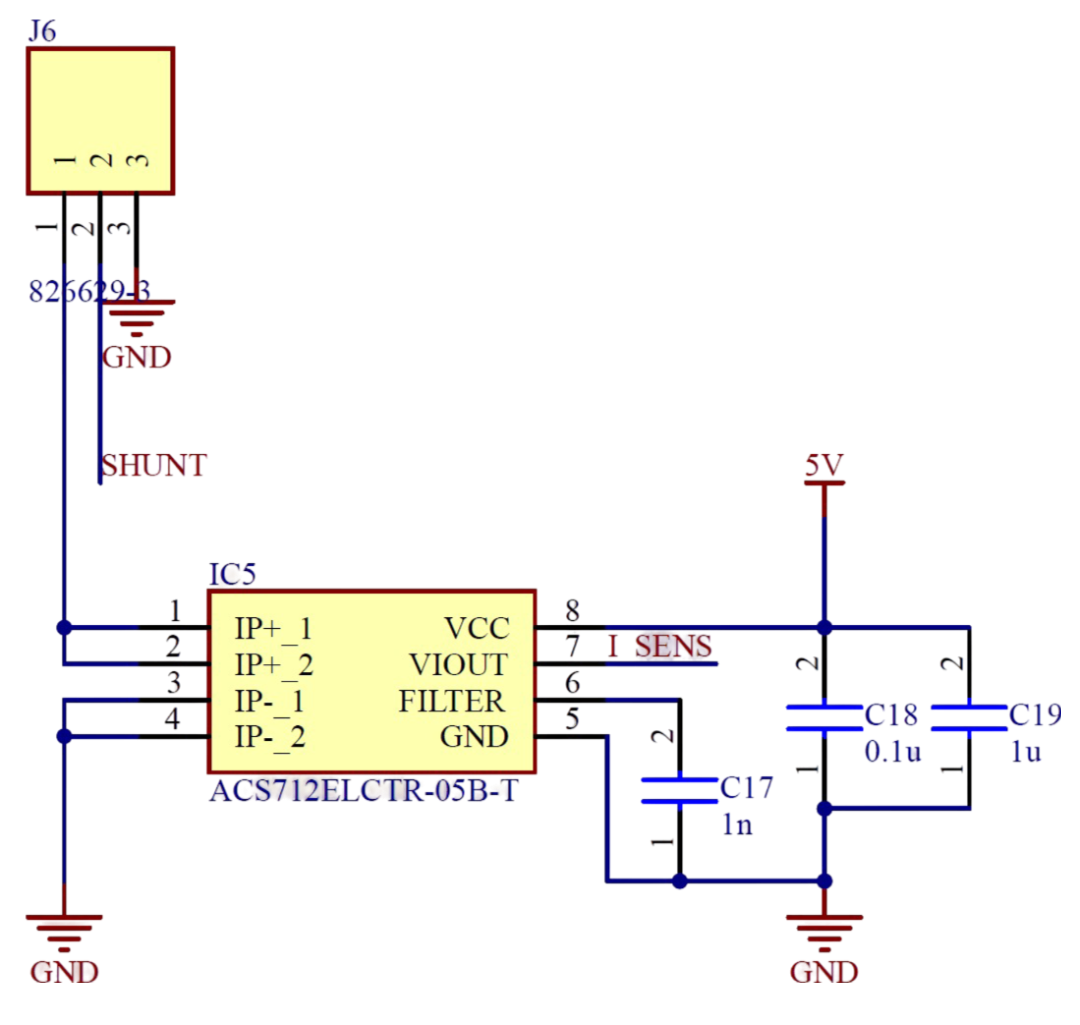
\includegraphics[width=0.5\textwidth]{inc/img/cur_sens.png}
\caption{Схема с датчиком тока ($SHUNT$ --- сигнал с фаз двигателя, $5V$ --- питание $5$ В, $I_{SENS}$ --- сигнал выхода датчика тока)}
\label{pic:cur_sens}
\end{figure}

Для измерения напряжения на фазах необходимо использовать делители напряжения для преобразования из диапазона $0-12$ В в диапазон $0-5$ В. Также устанавливается конденсатор для избавления от высокочастотных шумов. Схема изображена на Рисунке 

\begin{figure}[!h]
\centering
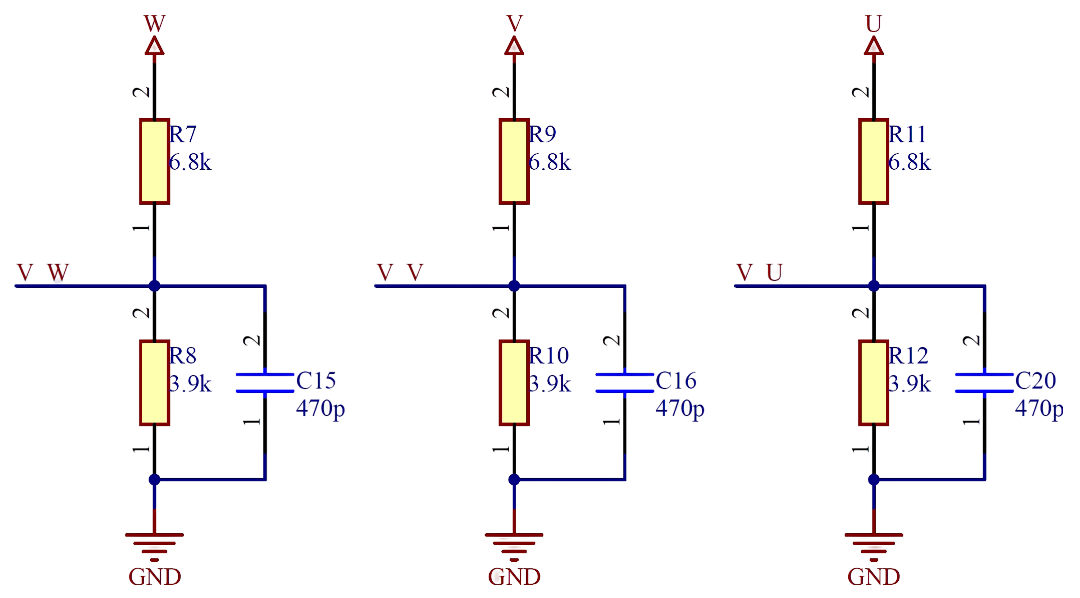
\includegraphics[width=0.7\textwidth]{inc/img/dr_dels.png}
\caption{Схема с делителями напряжения ($WVU$ --- фазы двигателя, $V_{VWU}$ --- сигналы с напряжениями фаз))}
\label{pic:dr_dels}
\end{figure}

\subsection{Подключение входов и выходов платы}

Питание платы осуществляется двумя уровнями напряжений --- $12$ и $5$ В. Первое идёт на питание двигателя и формируется блоком питания, второе служит для питания датчика тока и идёт от микроконтроллера. От микроконтроллера также идут сигналы для управления драйверами транзисторов.

От плату на входы АЦП микроконтроллера идут сигналы с датчика тока и делителей напряжения. Однако на плате напряжения выходных сигналов приведены в диапазоне $0-5$ В, а АЦП выбранного микроконтроллера работает с напряжениями $0-3,3$ В, поэтому не можем напрямую подключить сигналы с платы и необходимо использовать преобразователь логических уровней. Был выбран преобразователь на основе TXS108E.

\begin{figure}[!h]
\centering
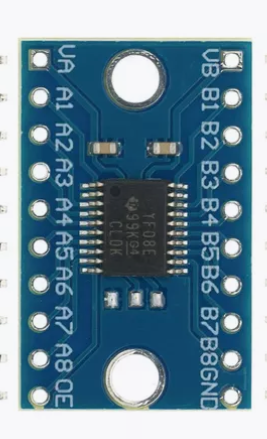
\includegraphics[width=0.3\textwidth]{inc/img/log_transf.png}
\caption{Преобразователь логических уровней на базе TXS108E}
\label{pic:log_transf}
\end{figure}

Подключение фаз двигателя осуществляется через 2-х контактный клеммник, как и напряжения питания $12$ В. Остальные сигналы подключаются посредством штырьевых разъёмов.

\subsection{Общий вид платы}

На Рисунке \ref{pic:dr_view1} приведён вид платы, сгенерированный в редакторе, а на Рисунке \ref{pic:dr_view2} изображена уже изготовленная и распаянная плата.

\begin{figure}[!h]
\centering
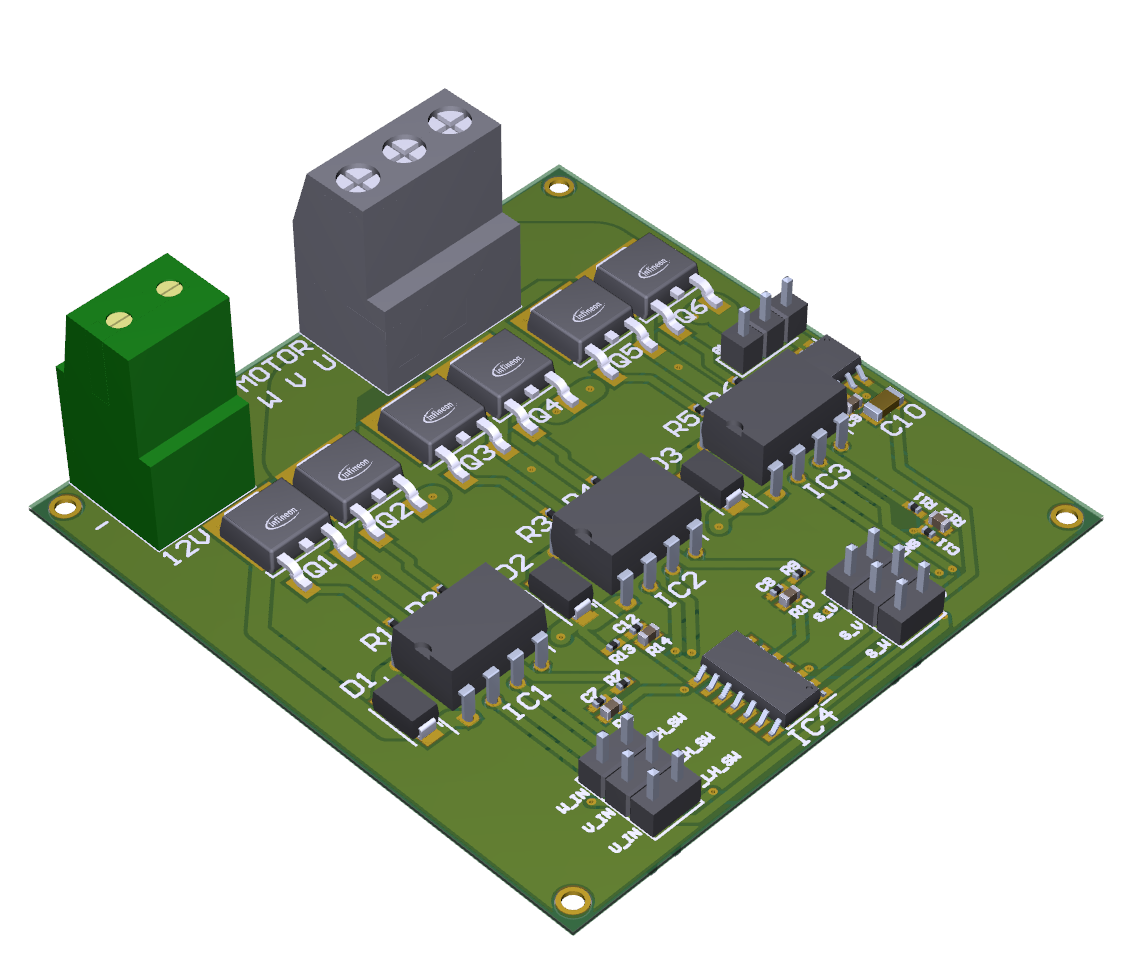
\includegraphics[width=0.7\textwidth]{inc/img/dr_view1.png}
\caption{Вид платы из Altium Designer}
\label{pic:dr_view1}
\end{figure}

\begin{figure}[!h]
\centering
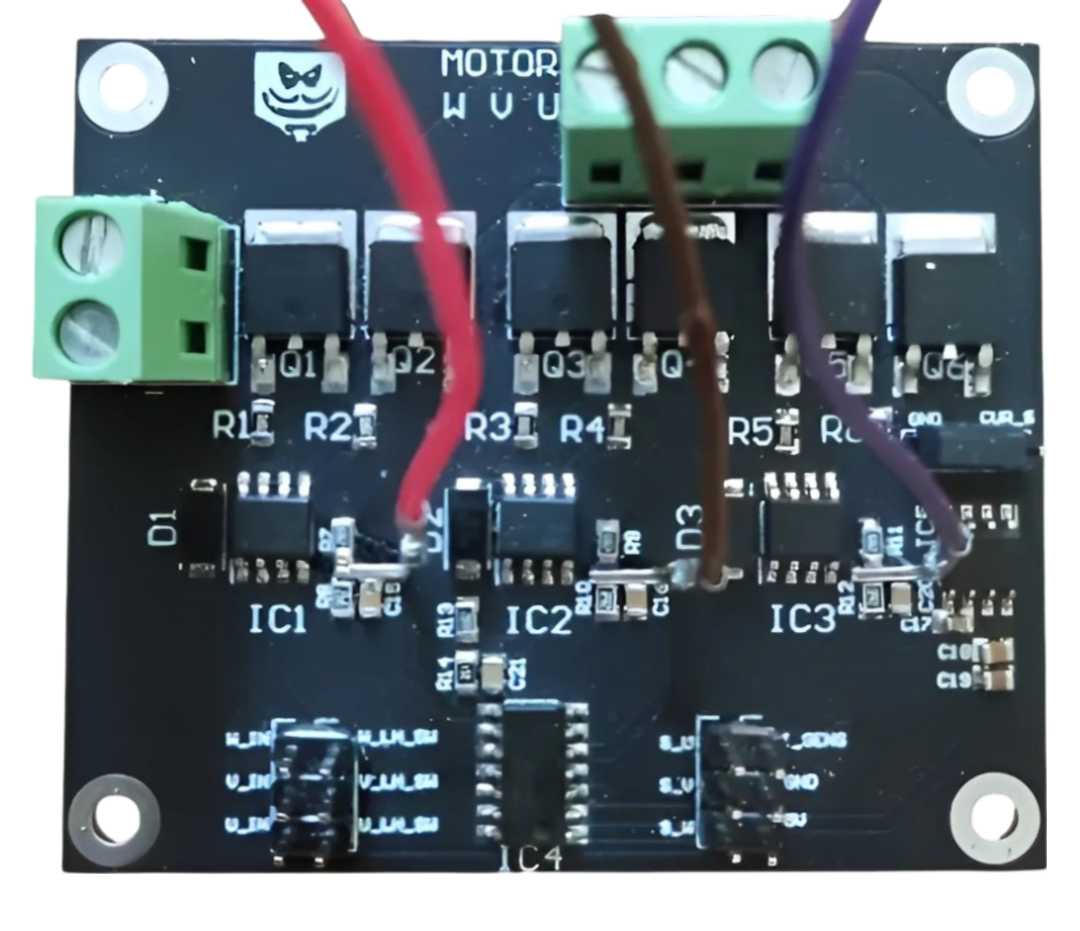
\includegraphics[width=0.7\textwidth]{inc/img/dr_view2.png}
\caption{Вид изготовленной платы}
\label{pic:dr_view2}
\end{figure}
\clearpage
\section{Вид стенда}

На основе выбранных компонентов и узлов был собран стенд для экспериментальных исследований, представленный на Рисунке \ref{pic:stand}.

\begin{figure}[!h]
\centering
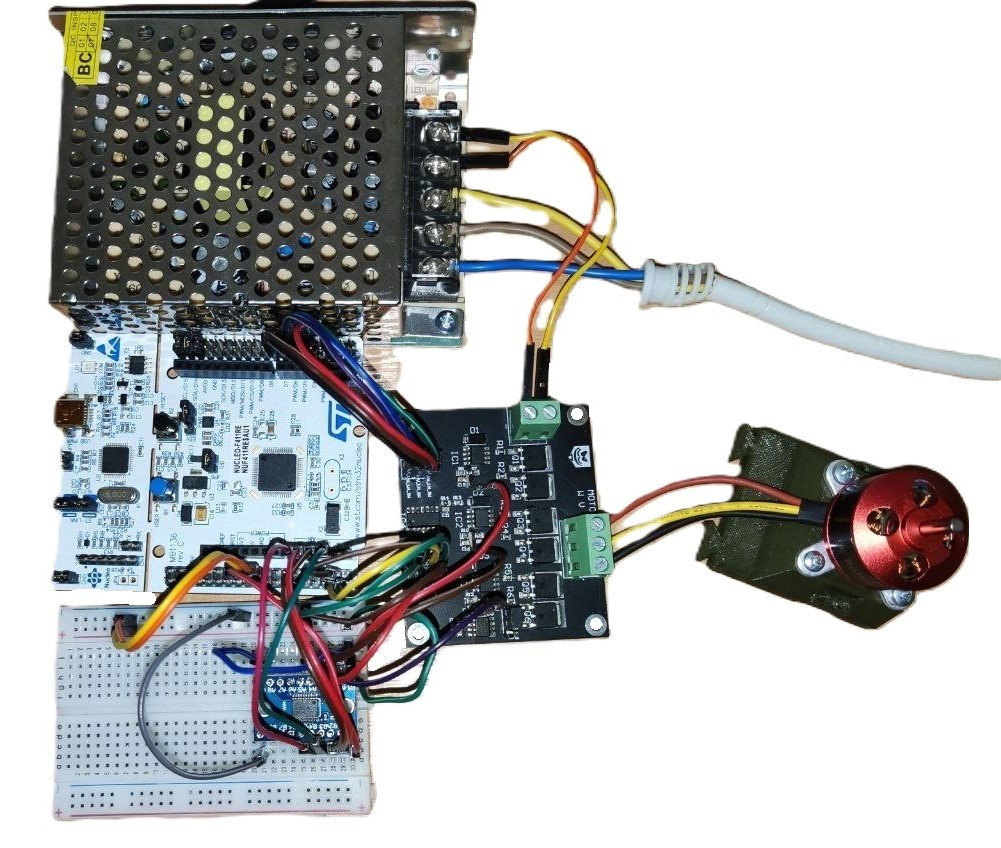
\includegraphics[width=0.7\textwidth]{inc/img/stand}
\caption{Экспериментальный стенд}
\label{pic:stand}
\end{figure}
%\chapter{Анализ работы конечного устройства}
\label{cha:chap6}

\section{Результаты работы устройства}

\section{Сравнение модели и реального устройства}


\backmatter %% Здесь заканчивается нумерованная часть документа и начинаются ссылки и
            
\Conclusion % заключение к отчёту
\thispagestyle{empty}

Был разработан алгоритм управления скоростью бесколлекторных бездатчиковых двигателей постоянного тока. 

Была составлена модель с использованием выбранного алгоритма в программном комплексе Matlab/Simulink и проведено моделирование. Моделирование проводилось при исходных параметрах двигателя, а также при вариации сопротивления и индуктивности статора для проверки робастных свойств. Во всех случаях получилось добиться желаемых показателей качества.

На основе модели был разработан экспериментальный стенд с учётом требований, предъявляемых в техническом задании, и проведено исследование его работы. В итоге, также получилось достичь желаемых показателей качества, что говорит об эффективности алгоритма в практической среде.

%% заключение

% % Список литературы при помощи BibTeX
% Юзать так:
%
% pdflatex rpz
% bibtex rpz
% pdflatex rpz

\bibliographystyle{ugost2008}
\bibliography{rpz}

%%% Local Variables: 
%%% mode: latex
%%% TeX-master: "rpz"
%%% End: 



\appendix   % Тут идут приложения

%\chapter{Емкостный датчик наклона}
\label{cha:appendix1}

\begin{figure}
\centering
\includegraphics[width=0.8\textwidth]{inc/img/pat1.png}
%\caption{Характеристики выбранного двигателя}
\end{figure}

%%% Local Variables: 
%%% mode: latex
%%% TeX-master: "rpz"
%%% End: 

%\chapter{Датчик наклона на основе ампулы}
\label{cha:appendix2}

\begin{figure}
\centering
\includegraphics[width=0.8\textwidth]{inc/img/pat2.png}
%\caption{Технические характеристики преобразователя частоты 8000M-2SR4GH}
\end{figure}

%%% Local Variables: 
%%% mode: latex
%%% TeX-master: "rpz"
%%% End: 

%\chapter{Датчик наклона на базе акселерометра}
\label{cha:appendix3}

\begin{figure}
\centering
\includegraphics[width=0.9\textwidth]{inc/img/pat3.png}
%\caption{Технические характеристики энкодера PRI 80H22}
\end{figure}

%%% Local Variables: 
%%% mode: latex
%%% TeX-master: "rpz"
%%% End: 

%\chapter{Датчик наклона на магнитах}
\label{cha:appendix4}

\begin{figure}
\centering
\includegraphics[width=0.8\textwidth]{inc/img/pat4.png}
%\caption{Технические характеристики энкодера PRI 80H22}
\end{figure}

%%% Local Variables: 
%%% mode: latex
%%% TeX-master: "rpz"
%%% End: 

%\chapter{Механический датчик наклона}
\label{cha:appendix5}

\begin{figure}
\centering
\includegraphics[width=0.8\textwidth]{inc/img/pat5.png}
%\caption{Технические характеристики энкодера PRI 80H22}
\end{figure}

%%% Local Variables: 
%%% mode: latex
%%% TeX-master: "rpz"
%%% End: 

%\chapter{Характеристики датчика LIS3DH}
\label{cha:appendix6}

\begin{figure}
\centering
\includegraphics[width=0.8\textwidth]{inc/img/dat.png}
%\caption{Технические характеристики энкодера PRI 80H22}
\end{figure}

%%% Local Variables: 
%%% mode: latex
%%% TeX-master: "rpz"
%%% End: 


\end{document}

%%% Local Variables:
%%% mode: latex
%%% TeX-master: t
%%% End:
